%% Adaptado a partir de :
%DIF LATEXDIFF DIFFERENCE FILE
%DIF DEL versao_antiga/main-texto-completo.tex   Sun Aug 28 21:44:18 2022
%DIF ADD versao_nova/main-texto-completo.tex     Sun Aug 28 19:52:55 2022
%%    abtex2-modelo-trabalho-academico.tex, v-1.9.2 laurocesar
%% para ser um modelo para os trabalhos no IFSP-SPO

\documentclass[
    % -- opções da classe memoir --
    12pt,               % tamanho da fonte
    openright,          % capítulos começam em pág ímpar (insere página vazia caso preciso)
    %twoside,            % para impressão em verso e anverso. Oposto a oneside
    oneside,
    a4paper,            % tamanho do papel. 
    % -- opções da classe abntex2 --schwinn
    % Opções que não devem ser utilizadas na versão final do documento
    %draft,              % para compilar mais rápido, remover na versão final
    paginasA3,  % indica que vai utilizar paginas em A3 
    BIBLATEX,           % indica para utilizar BIBLATEX em vez do abntex2cite
    REFINDENT,          % não fica exatamente no formato da ABNT, mas melhora muito a formatação
                        % não utilizar REFINDENT na versão final
    MODELO,             % indica que é um documento modelo então precisa dos geradores de texto
    TODO,               % indica que deve apresentar lista de pendencias 
    % -- opções do pacote babel --
    english,            % idioma adicional para hifenização
    brazil              % o último idioma é o principal do documento
%DIF 24-25c24
%DIF <     ]{ifsp-spo-inf-cemi} % ajustar de acordo com o modelo desejado para o curso
%DIF < \AtBeginDocument
%DIF -------
    ]{ifsp-spo-inf-ctds} % ajustar de acordo com o modelo desejado para o curso %DIF > 
%DIF -------

% ---
% Informações de dados para CAPA e FOLHA DE ROSTO
% ---
\titulo{GARAGE LAUNCHER - DIVERSAGENTE}

% Trabalho individual
%\autor{AUTOR DO TRABALHO}

% Trabalho em Equipe
% ver também https://github.com/abntex/abntex2/wiki/FAQ#como-adicionar-mais-de-um-autor-ao-meu-projeto
\renewcommand{\imprimirautor}{
\begin{tabular}{lr}
GABRIEL DE MORAIS RUIZ & SP3046893 \\
GRAZIELLI LIMA BERTI & SP3046966 \\
GUSTAVO LOURENÇO DE FREITAS & SP3049566 \\
JOÃO VITOR SILVA BISPO & SP3052672 \\
%DIF 43c42
%DIF < TAYNA RITA DE FRANÇA SOUZA & SP3050173\\
%DIF -------
TAYNA RITA DE FRANÇA SOUZA & SP3050173 \\ %DIF > 
%DIF -------
VINICIUS ALMEIDA SOARES & SP3046991 \\
VIVIANE DE SANTANA QUEIROZ & SP3053601 \\
\end{tabular}
}


%DIF 50c49
%DIF < \disciplina{PI1A5 - Projeto Integrado I}
%DIF -------
\disciplina{PIA5 - Projeto Integrado I} %DIF > 
%DIF -------

%DIF 52c51-54
%DIF < \preambulo{Documentação da aplicação apresentada no curso de Tecnologia em Análise e Desenvolvimento de Sistemas do Instituto Federal de São Paulo, da disciplina de PIA5.}
%DIF -------
\preambulo{Documentação da aplicação apresentada no %DIF > 
curso de Tecnologia em Análise e Desenvolvimento %DIF > 
de Sistemas do Instituto Federal de %DIF > 
São Paulo, da disciplina de Projeto Integrado I.} %DIF > 
%DIF -------

%DIF 54c56
%DIF < \data{23/05/2022}
%DIF -------
\data{2022} %DIF > 
%DIF -------

% Definir o que for necessário e comentar o que não for necessário
% Utilizar o Nome Completo, abntex tem orientador e coorientador
% então vão ser utilizados na definição de professor
\renewcommand{\orientadorname}{Professor:}
\orientador{JOSÉ BRAZ DE ARAUJO}
\renewcommand{\coorientadorname}{Professor:}
\coorientador{MARCELO TAVARES DE SANTANA}


% ---


% informações do PDF
\makeatletter
\hypersetup{
        %pagebackref=true,
        pdftitle={\@title}, 
        pdfauthor={\@author},
        pdfsubject={\imprimirpreambulo},
        pdfcreator={LaTeX with abnTeX2 using IFSP model},
        pdfkeywords={abnt}{latex}{abntex}{abntex2}{IFSP}{\ifspprefixo}{trabalho acadêmico}, 
        colorlinks=true,            % false: boxed links; true: colored links
        linkcolor=blue,             % color of internal links
        citecolor=blue,             % color of links to bibliography
        filecolor=magenta,              % color of file links
        urlcolor=blue,
        bookmarksdepth=4
}
\makeatother
% --- 

% carregando aqui referencias quando utilizando BIBLATEX
\IfPackageLoaded{biblatex}{%
\addbibresource{referencias.bib}
\addbibresource{exemplos/abntex2-doc-abnt-6023.bib}
}{}

% ----
% Início do documento
% ----
%DIF PREAMBLE EXTENSION ADDED BY LATEXDIFF
%DIF UNDERLINE PREAMBLE %DIF PREAMBLE
\RequirePackage[normalem]{ulem} %DIF PREAMBLE
\RequirePackage{color}\definecolor{RED}{rgb}{1,0,0}\definecolor{BLUE}{rgb}{0,0,1} %DIF PREAMBLE
\providecommand{\DIFadd}[1]{{\protect\color{blue}\uwave{#1}}} %DIF PREAMBLE
\providecommand{\DIFdel}[1]{{\protect\color{red}\sout{#1}}}                      %DIF PREAMBLE
%DIF SAFE PREAMBLE %DIF PREAMBLE
\providecommand{\DIFaddbegin}{} %DIF PREAMBLE
\providecommand{\DIFaddend}{} %DIF PREAMBLE
\providecommand{\DIFdelbegin}{} %DIF PREAMBLE
\providecommand{\DIFdelend}{} %DIF PREAMBLE
\providecommand{\DIFmodbegin}{} %DIF PREAMBLE
\providecommand{\DIFmodend}{} %DIF PREAMBLE
%DIF FLOATSAFE PREAMBLE %DIF PREAMBLE
\providecommand{\DIFaddFL}[1]{\DIFadd{#1}} %DIF PREAMBLE
\providecommand{\DIFdelFL}[1]{\DIFdel{#1}} %DIF PREAMBLE
\providecommand{\DIFaddbeginFL}{} %DIF PREAMBLE
\providecommand{\DIFaddendFL}{} %DIF PREAMBLE
\providecommand{\DIFdelbeginFL}{} %DIF PREAMBLE
\providecommand{\DIFdelendFL}{} %DIF PREAMBLE
%DIF LISTINGS PREAMBLE %DIF PREAMBLE
\RequirePackage{listings} %DIF PREAMBLE
\RequirePackage{color} %DIF PREAMBLE
\lstdefinelanguage{DIFcode}{ %DIF PREAMBLE
%DIF DIFCODE_UNDERLINE %DIF PREAMBLE
  moredelim=[il][\color{red}\sout]{\%DIF\ <\ }, %DIF PREAMBLE
  moredelim=[il][\color{blue}\uwave]{\%DIF\ >\ } %DIF PREAMBLE
} %DIF PREAMBLE
\lstdefinestyle{DIFverbatimstyle}{ %DIF PREAMBLE
	language=DIFcode, %DIF PREAMBLE
	basicstyle=\ttfamily, %DIF PREAMBLE
	columns=fullflexible, %DIF PREAMBLE
	keepspaces=true %DIF PREAMBLE
} %DIF PREAMBLE
\lstnewenvironment{DIFverbatim}{\lstset{style=DIFverbatimstyle}}{} %DIF PREAMBLE
\lstnewenvironment{DIFverbatim*}{\lstset{style=DIFverbatimstyle,showspaces=true}}{} %DIF PREAMBLE
%DIF END PREAMBLE EXTENSION ADDED BY LATEXDIFF

\begin{document}

% Retira espaço extra obsoleto entre as frases.
\frenchspacing

%DIF < somente para o exemplo, fica primeiro
\DIFdelbegin %DIFDELCMD < 

%DIFDELCMD < %%%
\DIFdelend % -- lista de pendencias gerada pelo todonotes
% -- altere opções do usepackage para remover na versão final....
%DIF > \listoftodos
%DIF > \todo[inline]{remover lista de todo da versão final...}
%DIF > \newpage

\DIFdelbegin %DIFDELCMD < \newpage
%DIFDELCMD < 

%DIFDELCMD < %%%
\DIFdelend % ----------------------------------------------------------
% ELEMENTOS PRÉ-TEXTUAIS
% ----------------------------------------------------------
\DIFdelbegin %DIFDELCMD < \pretextual
%DIFDELCMD < %%%
\DIFdelend %DIF > \pretextual

% ---
% Capa
% ---
\imprimircapa

\DIFdelbegin %DIFDELCMD < \newcounter{todocounter}
%DIFDELCMD < \newcommand{\todonum}[2][]
%DIFDELCMD < {\stepcounter{todocounter}\todo[#1]{\thetodocounter: #2}}
%DIFDELCMD < %%%
\DIFdelend %DIF > \newcounter{todocounter}
%DIF > \newcommand{\todonum}[2][]
%DIF > {\stepcounter{todocounter}\todo[#1]{\thetodocounter: #2}}

% ---
\DIFdelbegin %DIFDELCMD < 

%DIFDELCMD < %%%
%DIF <  ---
\DIFdelend % Folha de rosto
% (o * indica que haverá a ficha bibliográfica)
% ---
\imprimirfolhaderosto
%\imprimirfolhaderosto*
% ---

% Quando registrado na biblioteca
%\input{pre-fichacatalografica}

%Caso necessário
%\input{pre-errata}

%Obrigatório para trabalhos com bancas oficiais
%\input{pre-aprovacao}

% ---- opcionais 
%DIF >  ---
%DIF >  Dedicatória
%DIF >  ---
\DIFaddbegin \begin{dedicatoria}
   \vspace*{\fill}
   \centering
   \noindent
   \textit{ \DIFadd{Este trabalho é dedicado ao público neurodiverso que}\\
   \DIFadd{merece, assim como todos, respeito.}} 
\DIFaddend 

%DIF > \todonum[inline]{colocar sua dedicatoria}
   \DIFaddbegin 

   \vspace*{\fill}


\end{dedicatoria}
%DIF >  ---
%DIF >  ---
%DIF >  Agradecimentos
%DIF >  ---
\begin{agradecimentos}
%DIF > \todonum[inline]{colocar seus agradecimentos}
\DIFadd{Os principais agradecimentos são direcionados ao casal Dario e Isis França, irmão e cunhada, respectivamente, da Product Owner Tayna França, que foram a base e motivação para a criação do projeto diversaGente e que foram de enorme valor para a compreensão da realidade das pessoas neurodiversas e das que estão em volta delas.
}

\DIFadd{Os agradecimentos especiais se direcionam aos professores José Braz de Araújo e Marcelo Tavares de Santana, que, durante todo o desenvolvimento do projeto, estiveram abertos a apoiar e aconselhar com o que fosse necessário, passando orientações e feedbacks de forma clara e direta.
}

\DIFadd{Por fim, agradecimentos à todos que, de alguma forma, contribuíram para que o projeto fosse concluído.
}

\end{agradecimentos}
%DIF >  ---
%DIF > \input{pre-epigrafe}

\DIFaddend % -- resumo obrigatório
% ---
% RESUMOS
% ---

% resumo em português
\setlength{\absparsep}{18pt} % ajusta o espaçamento dos parágrafos do resumo
\DIFaddbegin \begin{resumo}
\DIFaddend 

%DIF < \resumo
%DIF < \cleardoublepage
\DIFaddbegin \DIFadd{Com o crescimento exponencial do uso da internet na última década, as redes sociais se mostraram o maior centro de socialização da sociedade moderna, local em que são pautadas uma infinidade de assuntos. Percebendo que, em meio a essa infinidade, existe a necessidade de evidenciação de algumas dessas pautas por vezes negligenciadas frente aos tópicos dominantes nas redes, surge o diversaGente. Esse é um aplicativo de rede social focado na melhoria de vida de pessoas com neurodiversidades e suas famílias a partir da criação de um ambiente em que elas sintam-se confortáveis para trocar experiências. E para tornar esse app possível, a metodologia ágil seguida para organizar e desenvolver do projeto baseia-se Scrum. Além disso, toda a documentação foi construída de acordo com as regras }\ac{ABNT} \DIFadd{e as tecnologias utilizadas no desenvolvimento integram o ecossistema JavaScript, as quais incluem React Native, Typescript, Node.JS, Nest.JS e Prisma.
}\DIFaddend 

 \DIFaddbegin \textbf{\DIFadd{Palavras-chaves}}\DIFadd{: rede social. neurodiversidades. projeto.
}

\end{resumo}

%DIF >  resumo em inglês
\begin{resumo}[Abstract]
 \begin{otherlanguage*}{english}

\DIFadd{With the exponential growth of internet usage in the last decade, social networks proved to be the biggest center of socialization of modern society, where it can be find a multitude of subjects. Realizing that in the midst of this infinity there is a necessity of highlighting some of these themes that are sometimes neglected in comparison to the mainstream topics on the social media, the diversaGente appears. It is a social network app focused on improving the lives of people with neurodiversities and their family by creating an environment where they feel comfortable to exchange experiences. And to build this app, the agile methodology followed to organize and develop the project is based on Scrum. In addition, the complete documentation complies with the }\ac{ABNT} \DIFadd{rules and the technologies used in development are part of the JavaScript ecosystem, which includes React Native, Typescript, Node.JS, Nest.JS and Prisma.
}

   \textbf{\DIFadd{Keywords}}\DIFadd{: social networks. neurodiversities. project.
 }\end{otherlanguage*}
\end{resumo}


\DIFaddend % ---
% inserir lista de ilustrações
% ---
\pdfbookmark[0]{\listfigurename}{lof}
\listoffigures*
\cleardoublepage
% ---

% ---
% inserir lista de tabelas
%DIF <  ---%
%DIF >  ---
%\pdfbookmark[0]{\listtablename}{lot}
%\listoftables*
%\cleardoublepage
% ---

% ---
% inserir lista de quadros
% ---
\pdfbookmark[0]{\listofquadrosname}{loq}
\listofquadros*
\cleardoublepage
% ---

% ---
%DIF >  inserir lista de abreviaturas e siglas
%DIF >  ATENCAO o SHARELATEX/OVERLEAF GERA O GLOSSARIO SOMENTE UMA VEZ
%DIF >  CASO SEJA FEITA ALGUMA ALTERAÇÃO NA LISTA DE SIGLAS É NECESSARIO UTILIZAR A OPÇÃO :
%DIF >  "Clear Cached Files" DISPONIVEL NA VISUALIZAÇÃO DOS LOGS 
%DIF >  ---
%DIF >  https://www.sharelatex.com/learn/Glossaries
\DIFaddbegin 


\ifdef{\printnoidxglossary}{
    \printnoidxglossary[type=\acronymtype,title=Lista de abreviaturas e siglas,style=siglas]
    \cleardoublepage
}{}


%DIF > \todo[inline]{Remover lista de símbolos se não for necessária}
%DIF > \input{pre-simbolos}


%DIF >  ---
\DIFaddend % inserir o sumario
% ---
\pdfbookmark[0]{\contentsname}{toc}
\tableofcontents*
\cleardoublepage
% ---


% ----------------------------------------------------------
% ELEMENTOS TEXTUAIS
% ----------------------------------------------------------
\textual


% ----------------------------------------------------------
% Introdução
% ----------------------------------------------------------
\DIFaddbegin \chapter[Introdução]{\DIFadd{Introdução}}
\DIFaddend 

\DIFdelbegin \chapter{\DIFdel{Introdução}}
%DIFAUXCMD
\addtocounter{chapter}{-1}%DIFAUXCMD
%DIFDELCMD < 

%DIFDELCMD < %%%
\DIFdelend Dispositivos móveis são amplamente utilizados pelos brasileiros, em 2019 82,7\% dos domicílios brasileiros possuíam acesso à Internet, e 98,6\% deles o faziam através de um telefone celular \DIFdelbegin \DIFdel{(IBGE, 2019)}\DIFdelend \DIFaddbegin \DIFadd{\mbox{%DIFAUXCMD
\cite{ibge2019}}\hspace{0pt}%DIFAUXCMD
}\DIFaddend . Com este alto índice de uso surge também a grande popularidade das redes sociais no país e, por consequência da facilidade de disseminar informação, a necessidade de encontrar lugares confiáveis para se compartilhar e receber informações.

As redes sociais possibilitam a interação de milhões de pessoas, integrando grupos variados de diferentes lugares em um único ambiente virtual. Essas redes funcionam muito bem para lidar com as necessidades de interação da maioria das pessoas, mas não é possível afirmar que se encaixam perfeitamente para todos, afinal, existem públicos que requerem atenção diferenciada, um exemplo deles são as pessoas neurodiversas, que vivenciam uma rotina completamente destoante do convencional.

As barreiras e preconceitos que pessoas \DIFdelbegin \DIFdel{neurodivergentes }\DIFdelend \DIFaddbegin \DIFadd{neurodiversas }\DIFaddend enfrentam na sociedade se iniciam já na dificuldade de acesso à informações corretas e confiáveis sobre o próprio termo que as englobam: neurodiversidade. Um termo designado à condição de pessoas cuja neurobiologia se desenvolveu de forma atípica em relação a um parâmetro médico e biológico que se designa como desenvolvimento normal na espécie humana. O Transtorno de Déficit de \DIFdelbegin \DIFdel{atenção }\DIFdelend \DIFaddbegin \DIFadd{Atenção e Hiperatividade }\DIFaddend (TDAH) e o Transtorno do Espectro Autista (TEA) são exemplos de diagnósticos comuns às pessoas neurodiversas e, apesar de todo o avanço científico dos últimos anos que possibilitam cada vez maior qualidade de vida, existem muitas barreiras de âmbito social que estas pessoas ainda enfrentam. Diante desse cenário, a socialização de milhares de pessoas neurodiversas é prejudicada e, muitas vezes, descredibilizada, e dado que o ser humano é um ser inerentemente social, o que ocorre é que elas têm uma necessidade elementar debilitada e por inúmeras vezes ignorada \DIFaddbegin \DIFadd{\mbox{%DIFAUXCMD
\cite{kanner43}}\hspace{0pt}%DIFAUXCMD
}\DIFaddend .

\DIFdelbegin \DIFdel{Pela existência das condições ditas é que o diversaGente se mostra um lugar cordial para pais, responsáveis e para as próprias pessoas neurodiversas, com o intuito de tornar-se um local disponível para que todos consigam compartilhar suas experiências, sejam elas experiências ou dicas de vida a serem relatadas por meio do fórum ou experiências vividas em lugares específicos das quais queiram falar sobre e/ou fazer uma avaliação - pontos positivos no atendimento de um restaurante ou profissional de saúde, por exemplo.
}%DIFDELCMD < 

%DIFDELCMD < %%%
\section{\DIFdel{Contextualização}}
%DIFAUXCMD
\addtocounter{section}{-1}%DIFAUXCMD
%DIFDELCMD < 

%DIFDELCMD < %%%
\DIFdel{O uso dos aparelhos móveis para realizar o acesso à internet cresceu significativamente no Brasil. Estes dispositivos se tornaram o principal meio de acesso à internet, usado pela grande maioria da população brasileira. As informações são da Pesquisa Nacional por Amostra de Domicílios Contínua - Tecnologia da Informação e Comunicação (PNAD Contínua TIC, 2018). Concomitantemente a isso, as redes sociais têm ganhado maior número de usuários e, consequentemente, maior relevância, modificando de maneira brusca a forma de se comunicar e socializar, as pessoas encontraram nos aplicativos de redes sociais uma nova forma de praticar antigos hábitos e atividades que são inerentes à elas, mas que variam de acordo com a necessidade de cada grupo. Em concordância com a necessidade de adaptação de grupos específicos, o aplicativo diversaGente é uma rede social com o foco voltado, principalmente, aos pais de crianças neurodiversas, ou seja, direcionada a um público específico de pessoas, mirando a busca por um maior engajamento e atenção para com este grupo. Ao se dispor como apoiador dessa busca, o diversaGente traz consigo a responsabilidade, não só de disponibilizar uma plataforma agradável e funcional, mas também de servir como fonte de informação e ambiente de discussão sobre o tema,  transmitindo maior volume e qualidade dessas informações, assim como a facilitando a comunicação entre esse nicho de pessoas.
}%DIFDELCMD < 

%DIFDELCMD < %%%
\section{\DIFdel{Problematização}}
%DIFAUXCMD
\addtocounter{section}{-1}%DIFAUXCMD
%DIFDELCMD < 

%DIFDELCMD < %%%
\DIFdel{Todo pai, mãe e }\DIFdelend \DIFaddbegin \DIFadd{Todo }\DIFaddend responsável \DIFdelbegin \DIFdel{de }\DIFdelend \DIFaddbegin \DIFadd{por }\DIFaddend uma criança \DIFdelbegin \DIFdel{diagnosticada com alguma neurodiversidade compreende e sente a dificuldade de receber esse primeiro }\DIFdelend \DIFaddbegin \DIFadd{neurodiversa compreende a dificuldade existente desde o momento do }\DIFaddend diagnóstico\DIFdelbegin \DIFdel{. Este momento costuma ser um misto de emoções, o medo do que irá acontecer deste momento em diante e a dúvida sobre como lidar com a }\DIFdelend \DIFaddbegin \DIFadd{, momento que traz uma enorme insegurança sobre como se dará o futuro da }\DIFaddend criança\DIFdelbegin \DIFdel{são os sentimentos mais comuns. Estes são sentimentos comuns quando se recebem informações desconhecidas }\DIFdelend \DIFaddbegin \DIFadd{, }\DIFaddend até \DIFdelbegin \DIFdel{então. No meio em que vivemos}\DIFdelend \DIFaddbegin \DIFadd{questões vistas como básicas do dia a dia. Atualmente}\DIFaddend , pouco se fala sobre \DIFaddbegin \DIFadd{as }\DIFaddend neurodiversidades, mas com \DIFdelbegin \DIFdel{um pouco de pesquisa descobrimos que muitas }\DIFdelend \DIFaddbegin \DIFadd{pouca pesquisa pode-se descobrir que várias das }\DIFaddend pessoas que apresentam essas condições \DIFdelbegin \DIFdel{, }\DIFdelend podem ter uma vida \DIFdelbegin \DIFdel{normal, }\DIFdelend \DIFaddbegin \DIFadd{dita socialmente como normal, conseguindo }\DIFaddend brincar, estudar, trabalhar e construir relacionamentos \DIFaddbegin \DIFadd{sólidos}\DIFaddend , assim como \DIFdelbegin \DIFdel{qualquer outra pessoa . A única }\DIFdelend \DIFaddbegin \DIFadd{outra pessoa não neurodiversa. O ponto de }\DIFaddend diferença é que\DIFdelbegin \DIFdel{a pessoa diagnosticada com transtorno global de desenvolvimento se desenvolve }\DIFdelend \DIFaddbegin \DIFadd{, aquele que é diagnosticado com alguma divergência neurológica se desenvolve psicologicamente }\DIFaddend de forma específica, \DIFdelbegin \DIFdel{muitas vezes com uma }\DIFdelend \DIFaddbegin \DIFadd{que varia de acordo com a neurodivergência em questão, e, muitas vezes, com alguma }\DIFaddend preocupação a mais em relação ao ambiente e estímulos \DIFdelbegin \DIFdel{. Para que seja mais fácil receber esse diagnóstico e para nenhum pai se sentir sozinho estamos criando um aplicativo de rede social voltada para paise }\DIFdelend \DIFaddbegin \DIFadd{externos (barulhos, toques e gestos, por exemplo). 
}

\DIFadd{Pela existência das condições ditas é que o diversaGente se mostra um lugar cordial para pais, }\DIFaddend responsáveis \DIFdelbegin \DIFdel{de crianças neurodiversas. Para que juntos eles possam compartilhar informações e cuidados, quebrar o preconceito que sentem ao receber o diagnostico, buscar dicas de profissionais especializados em sua região com base em notas e opiniões, atividades úteis para o processo de aprendizado e principalmente entender que }\DIFdelend \DIFaddbegin \DIFadd{e para as próprias pessoas neurodiversas, que }\DIFaddend não \DIFdelbegin \DIFdel{é necessário se esconder, pois agora você faz parte de uma comunidade que te entende e apoia}\DIFdelend \DIFaddbegin \DIFadd{encontram com facilidade um ambiente em que tenham suas pautas evidenciadas e que possam encontrar pessoas com as mesmas questões e realidades}\DIFaddend .

\section{\DIFdelbegin \DIFdel{Objetivos}\DIFdelend \DIFaddbegin \DIFadd{Objetivo}\DIFaddend }

A falta de acesso à informação a respeito \DIFdelbegin \DIFdel{do autismo e outros transtornos de desenvolvimento como síndrome }\DIFdelend de \DIFaddbegin \DIFadd{neurodiversidades como o Autismo, Síndrome de }\DIFaddend Rett, \DIFdelbegin \DIFdel{distúrbio abrangente do desenvolvimento , síndrome }\DIFdelend \DIFaddbegin \DIFadd{Distúrbio Abrangente do Desenvolvimento , Síndrome }\DIFaddend de Timothy, \DIFdelbegin \DIFdel{síndrome do X-Frágil, síndrome }\DIFdelend \DIFaddbegin \DIFadd{Síndrome }\DIFaddend de Angelman, \DIFdelbegin \DIFdel{síndrome de Phelan-McDermid, síndrome de Asperger , TDAH ( }\DIFdelend \DIFaddbegin \DIFadd{Síndrome de Asperger e o }\DIFaddend Transtorno do Déficit de Atenção e \DIFdelbegin \DIFdel{/ou Hiperatividade), entre outras}\DIFdelend \DIFaddbegin \DIFadd{Hiperatividade}\DIFaddend , \DIFaddbegin \DIFadd{por exemplo, }\DIFaddend é um problema que todo \DIFdelbegin \DIFdel{responsável por crianças que se enquadram }\DIFdelend \DIFaddbegin \DIFadd{pai e mãe }\DIFaddend nessas condições \DIFdelbegin \DIFdel{enfrenta. A diversaGENTE }\DIFdelend \DIFaddbegin \DIFadd{enfrentam. O diversaGente }\DIFaddend tem como objetivo compartilhar conteúdos de qualidade com facilidade à informação para todos os pais e responsáveis de crianças neurodiversas. Como por exemplo notícias sobre neurodiversidade, boas escolas, médicos ao redor da sua localidade e aspectos de seus filhos divididos pelos pais em grandes fóruns de discussões. Não é uma rede social comum apenas para fazer amigos, é uma comunidade unida para troca de informação e conhecimento.


O aplicativo diversaGente tem como objetivo \DIFdelbegin \DIFdel{compartilhar conteúdos de qualidade para todos os pais eresponsáveis de crianças neurodiversas. Como}\DIFdelend \DIFaddbegin \DIFadd{tornar-se um local disponível para que todos consigam compartilhar suas experiências, sejam elas dicas de vida a serem relatadas por meio do fórum ou experiências vividas em lugares específicos das quais queiram falar sobre e/ou fazer uma avaliação, trazendo pontos positivos do atendimento de um restaurante ou profissional de saúde}\DIFaddend , por exemplo\DIFdelbegin \DIFdel{, notícias sobre neurodiversidade, boas escolas, médicos próximos a sua localidade e compartilhamento de experiências pelos paisem grandes fóruns de discussões}\DIFdelend .
\DIFdelbegin \DIFdel{Não é uma rede social comum apenas para fazer amigos, é }\DIFdelend \DIFaddbegin 

\DIFadd{Portanto, o diversaGente traz consigo a responsabilidade de transmitir maior volume e qualidade de informação acerca deste tema e, também, facilitar a comunicação entre esses pais, mães e responsáveis pelas crianças neurodiversas, criando, assim, }\DIFaddend uma comunidade unida em prol \DIFdelbegin \DIFdel{da troca de informação e conhecimento}\DIFdelend \DIFaddbegin \DIFadd{de uma causa e pronta para dar o apoio necessário àqueles que precisam}\DIFaddend .

\section{Justificativa}

Um estudo \DIFdelbegin \DIFdel{divulgado pela plataforma Cupom Válido, }\DIFdelend que reuniu dados da Hootsuite e WeAreSocial \DIFaddbegin \DIFadd{\mbox{%DIFAUXCMD
\cite{metropoles}}\hspace{0pt}%DIFAUXCMD
}\DIFaddend , mostra que o Brasil é o terceiro \DIFdelbegin \DIFdel{país no mundo que usa }\DIFdelend \DIFaddbegin \DIFadd{no ranking de países que mais utilizam as }\DIFaddend redes sociais. De acordo com o estudo, os brasileiros ficam, em média 3h42 por dia conectados, ficando atrás somente das Filipinas (4h15) e Colômbia (3h45).
Já em relação \DIFdelbegin \DIFdel{as }\DIFdelend \DIFaddbegin \DIFadd{às }\DIFaddend redes sociais, o Brasil conta com mais de 150 milhões de usuários, 70,3\% de sua população. O Sudeste aparece como a região com a maior taxa, cerca de 78\% dos usuários utilizam redes sociais.

Os dados em relação \DIFdelbegin \DIFdel{a neurodiversidade }\DIFdelend \DIFaddbegin \DIFadd{às neurodiversidades }\DIFaddend ainda não são muito divulgados\DIFaddbegin \DIFadd{, }\DIFaddend mas em relação ao autismo podemos destacar que uma em cada 44 crianças aos 8 anos de idade nos Estados Unidos é diagnosticada com o Transtorno do Espectro do Autismo (TEA), segundo relatório do CDC (Centro de Controle de Doenças e Prevenção), (publicado em 2.dez.2021). O número — com dados de 2018 — representa mais um aumento de 22\% em relação ao estudo anterior (1 para 54 — divulgado em 2020). Numa transposição dessa prevalência (de 2,3\% da população) para o Brasil, teríamos hoje cerca de 4,84 milhões de autistas no país. Porém, ainda não temos números de prevalência de autismo no Brasil.

%DIF < \begin{figure}[htb]
%DIF < 
 %DIF <    \centering
%DIF < 	\caption{\label{fig_arq_virado}Prevalência de autismo nos EUA 2021}
%DIF < 	\includegraphics[width=0.9\textwidth]{anexos/diversaGenteGrafico.png}
 %DIF <    \legend{Fonte: Equipe diversaGente}
%DIF < \end{figure}
\DIFaddbegin \begin{figure}[htb]
	\DIFaddendFL 

	\DIFaddbeginFL \centering
	\caption{\label{fig_arq_virado}\DIFaddFL{Prevalência de autismo nos }\ac{eua} \DIFaddFL{2021}}
	\includegraphics[width=0.9\textwidth]{anexos/diversaGenteGrafico.png}
\end{figure}

\DIFaddend Tendo isso em mente, \DIFdelbegin \DIFdel{desenvolvemos um aplicativo destinada }\DIFdelend \DIFaddbegin \DIFadd{o diversaGente é um aplicativo destinado }\DIFaddend aos pais e mães de crianças Neurodiversas  pois \DIFdelbegin \DIFdel{acreditamos }\DIFdelend \DIFaddbegin \DIFadd{é evidente }\DIFaddend que ter um filho com alguma neurodiversidade traz consigo \DIFdelbegin \DIFdel{alguns desafios. Como por exemplo}\DIFdelend \DIFaddbegin \DIFadd{vários desafios, como, por exemplo, }\DIFaddend encontrar escolas adequadas e \DIFdelbegin \DIFdel{uma lista longa }\DIFdelend \DIFaddbegin \DIFadd{um leque }\DIFaddend de profissionais especializados.
\DIFdelbegin \DIFdel{O objetivo do aplicativo é facilitar mesmo que um pouco nesse novo desafio, auxiliar com as escolhas de lugares utilizando notas de profissionais dadas por quem mais entende, os pais e mães. Apesar de existirem diversos grupos de discussões sobre neurodiversidades, muitas vezes as informações se perdem ou deixam de serem relevantes. 
Com nosso aplicativo esse problema não existira mais, terão informações atualizadas e filtros de fácil acesso. Outro ponto importante a ressaltar é que os pais poderão ser agrupados de acordo com o diagnóstico do transtorno global de desenvolvimento do seu filho, favorecendo a troca de informação relevante e mais precisa, facilitando a interação entre famílias. Criando assim uma rede de apoio, não só na escolha de médicos e escolas, mas na troca de informação e cuidados.
}\DIFdelend 

\section{Análise de concorrência refinada}

\DIFdelbegin \subsection{\DIFdel{Facebook}}
%DIFAUXCMD
\addtocounter{subsection}{-1}%DIFAUXCMD
\DIFdelend \DIFaddbegin \DIFadd{A seção tem o intuito de, através de pesquisas na internet, traçar um comparativo de aplicativos com finalidades similares às do diversaGente e evidenciar as particularidades que esta tem em relação às outras. É possível ver no }\autoref{tabela-comparativo} \DIFadd{as características de cada aplicação para melhor visualização. 
}\DIFaddend 

\DIFdelbegin \DIFdel{Facebook é uma }\DIFdelend \DIFaddbegin \DIFadd{O primeiro a ser comparado é o Facebook, além de ser uma }\DIFaddend das redes sociais mais usadas no Brasil e \DIFdelbegin \DIFdel{possui algumas ferramentas semelhantes ao nosso aplicativo }\DIFdelend \DIFaddbegin \DIFadd{no mundo, possui algumas características similares com o }\DIFaddend diversaGente, como \DIFdelbegin \DIFdel{fóruns, }\DIFdelend feed de postagem \DIFaddbegin \DIFadd{dentro de grupos}\DIFaddend , perfil pessoal \DIFdelbegin \DIFdel{, buscar usuários }\DIFdelend e opção de compartilhamento \DIFaddbegin \DIFadd{de postagens}\DIFaddend . 
\DIFdelbegin \DIFdel{Além de ser uma rede social muito utilizada ela também é muito completa.
}\DIFdelend 

\DIFdelbegin \subsection{\DIFdel{Twitter}}
%DIFAUXCMD
\addtocounter{subsection}{-1}%DIFAUXCMD
%DIFDELCMD < 

%DIFDELCMD < %%%
\DIFdel{Twitter}\DIFdelend \DIFaddbegin \DIFadd{Para o Twitter, }\DIFaddend uma rede social \DIFdelbegin \DIFdel{muito usada, principalmente }\DIFdelend \DIFaddbegin \DIFadd{que é um enorme fórum, muito utilizada }\DIFaddend entre os jovens, \DIFdelbegin \DIFdel{possui um feed de postagem, perfil pessoal,  buscar usuários e opção de compartilhamento mas o que mais se assemelha ao diversaGente }\DIFdelend \DIFaddbegin \DIFadd{porém não possui nenhuma página para criar grupos e se conversar sobre um assunto específico. Possui um filtro bem eficiente que }\DIFaddend é \DIFdelbegin \DIFdel{sua opção de ler noticia e ficar informado utilizado a rede social}\DIFdelend \DIFaddbegin \DIFadd{possível buscar por algo, caso alguém já tenha feito uma postagem sobre}\DIFaddend . 

\DIFdelbegin \subsection{\DIFdel{Tismoo.me}}
%DIFAUXCMD
\addtocounter{subsection}{-1}%DIFAUXCMD
%DIFDELCMD < 

%DIFDELCMD < %%%
\DIFdel{É a rede social que mais parece com diversaGente, pois é voltada para pais }\DIFdelend \DIFaddbegin \DIFadd{A Tismoo.me é a aplicação mais parecida com o diversaGente, possuindo também um fórum, nichada para o público de pais e responsáveis }\DIFaddend de crianças \DIFdelbegin \DIFdel{autistas, o nosso diferencial é que possuímos locaisavaliados e chat para }\DIFdelend \DIFaddbegin \DIFadd{pertencentes ao espectro autista. O diversaGente consegue se diferenciar do Tismoo.me pelas funcionalidades de avaliação de locais, sendo possível compartilhar a experiência do usuário e também pela }\DIFaddend interação \DIFdelbegin \DIFdel{entre os }\DIFdelend \DIFaddbegin \DIFadd{de chat em tempo real entre dois }\DIFaddend usuários. 

\DIFdelbegin \subsection{\DIFdel{Emergency Chat}}
%DIFAUXCMD
\addtocounter{subsection}{-1}%DIFAUXCMD
%DIFDELCMD < 

%DIFDELCMD < %%%
\DIFdel{Chat de emergência pode ser utilizado }\DIFdelend \DIFaddbegin \DIFadd{A característica principal da Emergency Chat é que pode ser utilizada }\DIFaddend em qualquer situação onde a fala é impossível, mas a comunicação ainda é necessária. \DIFdelbegin \DIFdel{Tem como público alvo pessoas neurodiversas. Mas não }\DIFdelend \DIFaddbegin \DIFadd{Não }\DIFaddend é necessariamente uma rede social, possui \DIFdelbegin \DIFdel{apenas }\DIFdelend um chat para comunicação.  

\DIFdelbegin \subsection{\DIFdel{TippyTalk}}
%DIFAUXCMD
\addtocounter{subsection}{-1}%DIFAUXCMD
%DIFDELCMD < 

%DIFDELCMD < %%%
\DIFdel{O aplicativo TippyTalk Community permite que o administrador ou gerente crie imagens que são }\DIFdelend \DIFaddbegin \DIFadd{O TippyTalk é um aplicativo voltado para pais ou responsáveis de crianças neurodiversas, principalmente aquelas com alguma dificuldade de comunicação verbal. Permite que um administrador crie imagens }\DIFaddend exclusivamente identificáveis e familiares para \DIFdelbegin \DIFdel{a pessoa que vive com a deficiência verbal. Voltada principalmente para pais de }\DIFdelend \DIFaddbegin \DIFadd{as }\DIFaddend crianças\DIFdelbegin \DIFdel{neurodiversas}\DIFdelend \DIFaddbegin \DIFadd{, apoiando na educação e treino de atividades/tarefas rotineiras}\DIFaddend . 

\DIFdelbegin \subsection{\DIFdel{The Autism Helper}}
%DIFAUXCMD
\addtocounter{subsection}{-1}%DIFAUXCMD
\DIFdel{O Autism Helper fornece recursos e comunidade para aqueles que procuram ajudar a criar a melhor vida }\DIFdelend \DIFaddbegin \DIFadd{O The Autism Helper também tem grande similaridade com o diversaGente porque é voltado para quem procura a facilitar, o máximo }\DIFaddend possível\DIFdelbegin \DIFdel{para }\DIFdelend \DIFaddbegin \DIFadd{, a vida de }\DIFaddend indivíduos \DIFdelbegin \DIFdel{com autismo.
}%DIFDELCMD < 

%DIFDELCMD < %%%
\DIFdel{O Autism Helper fornece recursos e comunidade para aqueles que procuram ajudar a criar a melhor vida possível para indivíduos com autismo. Além de ser voltado ao público neurodiverso, }\DIFdelend \DIFaddbegin \DIFadd{do espectro autista. O aplicativo }\DIFaddend possui fóruns para \DIFdelbegin \DIFdel{discussões }\DIFdelend \DIFaddbegin \DIFadd{discussão }\DIFaddend e perfil pessoal. 



\DIFdelbegin %DIFDELCMD < \begin{quadro}[htb]
%DIFDELCMD < %%%
\DIFdelend \DIFaddbegin \DIFadd{\
}\begin{quadro}[thb]
	\DIFaddend \centering
	\ABNTEXfontereduzida
	\DIFdelbegin %DIFDELCMD < \caption[Tabela Comparativa]{%%%
\DIFdel{Tabela Comparativa}\DIFdelend \DIFaddbegin \caption[Comparativo entre aplicações]{\DIFadd{Comparativo entre aplicações}\DIFaddend }	\DIFdelbegin %DIFDELCMD < \label{quadro-exemplo}
%DIFDELCMD < \begin{tabular}{|p{1.9cm}|p{1.7cm}|p{1.7cm}|p{1.5cm}|p{1.7cm}|p{1.7cm}|p{1.7cm}|p{1.7cm}|}
%DIFDELCMD <   %%%
\DIFdelend \DIFaddbegin \label{tabela-comparativo}

	\begin{tabular}{|l|c|c|c|c|c|c|c|}
		\DIFaddend \hline
		\thead{ } & \thead{diversa\\Gente} & \thead{Facebook}  & \thead{Twitter}  & \thead{Tismoo\\.me} & \thead{Emergency\\ Chat}  & \thead{Tippy\\ Talk}  & \thead{The \\Autism \\Helper}\\
		\hline
		Público Neurodiverso & X &  &  & X & X & X & X \\
		\hline
		Consultar Notícias & X &  & X & X &  &  &  \\
		\hline
		Fóruns & X & X &  & X &  &  & X \\
		\hline
		Locais Avaliados & X &  &  &  &  &  & \\
		\hline
		Chat & X & X & X &  & X & X &  \\
		\hline
		Feed de Postagem & X & X & X & X &  &  & X\\
		\hline
		Perfil Pessoal & X & X & X & X &  &  & \\
		\hline
		Buscar Usuários & X & X & X & X &  &  & \\
		\hline
		Compartilhar & X & X & X & X &  &  & X \\
		\hline
	\end{tabular}
\DIFaddbegin \fonte{Equipe diversaGente (2022)}
\DIFaddend \end{quadro}



% ---
% Capitulo de revisão de literatura
% ---
\DIFdelbegin %DIFDELCMD < 

%DIFDELCMD < %%%
%DIF <  ---
%DIFDELCMD < 

%DIFDELCMD < %%%
%DIF <  Para facilitar a manutenção é sempre melhore criar um arquivo por capitulo, para exemplo isso não é necessário 
%DIF <  Para facilitar a manutenção é sempre melhore criar um arquivo por capitulo, para exemplo isso não é necessário 
%DIFDELCMD < 

%DIFDELCMD < %%%
%DIF < ---------------------------------------------------------------------------------------
\DIFdelend \chapter{Revisão da Literatura}
\DIFaddbegin 

\DIFaddend Neste tópico \DIFaddbegin \DIFadd{iremos }\DIFaddend fazer um estudo e tirar observações mais a fundo a respeito da neurodiversidade. Relatar quando começou os estudos a respeito das pessoas neurodiversas e
entender como foi o papel da sociedade no passado, no que nisso acarretou e as mudanças necessárias que surgiram para chegar nos dias de hoje.
\DIFaddbegin 

\DIFaddend \section{Influência do termo}
As questões neurodiversas em toda sociedade sempre foi um assunto difícil de falar, principalmente porque no passado era tratado com "modelo de tragédia pessoal" \cite{oliver1990politics}. Dessa maneira, foi crescendo o indiferente e \DIFdelbegin \DIFdel{o }\DIFdelend inquestionável a respeito das pessoas que sofrem algum tipo de neurodiversidade. Entretanto, com os estudos, os teóricos que estudavam a causa mais fundo diziam que esse modelo social estaria equivocado, pois se deixar que essa percepção percorra nossa sociedade não irá trazer as necessárias responsabilidades sociais que devemos atingir para evitar esses equívocos. Sendo assim, essa mudança de responsabilidade para o comportamento com as neurodiversidades promove o empoderamentos do indivíduo e sendo assim ele ganha espaço para ser olhado pela sociedade e respeitado por elas.

\section{Virada de responsabilidades}
Um dos motivos que nos levou a trazer o tema da neurodiversidade para o \DIFdelbegin \DIFdel{nosso }\DIFdelend projeto final está na maneira que o assunto é tratado na sociedade. Há muitos tabus a serem derrubados. Se, por volta de 1960, ainda se culpavam os pais \DIFdelbegin \DIFdel{pela }\DIFdelend pelos seus filhos terem nascido com alguma neurodiversidade e, portanto, impossibilitava o surgimentos de movimentos que pudessem entender e ajudar os familiares, hoje temos algumas conquistas a serem celebradas como projetos de leis que protejam as pessoas neurodiversas graças aos estudos sobre deficiência nos anos 70 que desconstruiu um modelo de responsabilidade única para uma socialmente construída.\DIFdelbegin \DIFdel{\mbox{%DIFAUXCMD
\cite{ortega}
}\hspace{0pt}%DIFAUXCMD
}\DIFdelend \DIFaddbegin \DIFadd{\mbox{%DIFAUXCMD
\cite{ortega2008}}\hspace{0pt}%DIFAUXCMD
. }\DIFaddend Todavia, o preconceito, falta de informação e suporte ainda estão presentes no convívio social e dessa maneira, trazer uma rede social focada para sanar dúvidas e compartilhar informações e serviços torna-se esse assunto vivo diante a sociedade.

\section{Responsabilidade do Aplicativo}
Apontado no artigo de \cite{rios}, evidencia-se que no Brasil há um embate entre profissionais e pais a respeito do movimento neurodiverso, uma vez que a sociedade brasileira ainda está atrelada aos modelos ultrapassados lá da décadas de 1960. Dessa maneira, o diversaGente tem como objetivo tornar-se um ambiente de discussões e compartilhamento de informações sobre o assunto. Assim, o comprometimento na era digital que vivemos junto com a neurodiversidade nos remete ao compartilhamento de mais informações a respeito do assuntos com pessoas em diversos lugares, diversas famílias e culturas, pois em diversos artigos apresentam críticas a forma que os métodos atuais de tratamento são usados, uma vez que muitos tratamentos centram-se na deficiência e não na forma humana que deve ser tratado\DIFdelbegin \DIFdel{. \mbox{%DIFAUXCMD
\cite{machado}}\hspace{0pt}%DIFAUXCMD
}\DIFdelend \DIFaddbegin \DIFadd{\mbox{%DIFAUXCMD
\cite{machado}}\hspace{0pt}%DIFAUXCMD
. 
}\DIFaddend 


%DIF >  ---
\DIFaddbegin 


%DIF >  Para facilitar a manutenção é sempre melhore criar um arquivo por capitulo, para exemplo isso não é necessário 
%DIF >  Para facilitar a manutenção é sempre melhore criar um arquivo por capitulo, para exemplo isso não é necessário 

%DIF > ---------------------------------------------------------------------------------------


%DIF >  Para facilitar a manutenção é sempre melhore criar um arquivo por capitulo, para exemplo isso não é necessário 

%DIF > ---------------------------------------------------------------------------------------
\DIFaddend \chapter{Gestão do projeto}

A metodologia \DIFdelbegin \DIFdel{que a equipe escolheu para ser usado é o }\DIFdelend \DIFaddbegin \DIFadd{de gestão de projetos escolhida foi baseada no }\DIFaddend Scrum. Primeiramente pelo fato \DIFdelbegin \DIFdel{de ser ágil e }\DIFdelend \DIFaddbegin \DIFadd{da metodologia prezar a independência de todos da equipe, pela rapidez, agilidade de agregar valor para o cliente e produto final e }\DIFaddend também \DIFdelbegin \DIFdel{por estarmos desenvolvendo }\DIFdelend \DIFaddbegin \DIFadd{pelo desenvolvimento de }\DIFaddend um projeto no qual haverá necessidade de programar uma rede social e o Scrum atualmente é amplamente \DIFdelbegin \DIFdel{utilizado }\DIFdelend \DIFaddbegin \DIFadd{utilizada }\DIFaddend por equipes de desenvolvedores e \DIFdelbegin \DIFdel{também }\DIFdelend por ser a que os membros da equipe estão mais habituado a trabalhar.

Como foi decidido pela metodologia ágil Scrum, existe uma “hierarquia” e responsabilidades para que o desenvolvimento seja o mais eficiente possível. Para a nossa equipe há os cargos de Scrum Master, Product Owner e Desenvolvedores.

\begin{itemize}
	\item Scrum Master sendo o responsável para que a estrutura do Scrum seja seguida e realizada. Tira empecilhos de membros da equipe para que o desenvolvimento não seja comprometido, verifica a necessidade de adaptação do Scrum e obter um melhor fluxo de trabalho. O Gustavo Freitas ficou com a função de ser o Scrum Master do time.

	\item Tayna França Soza é a Product Owner (PO) da equipe e “representa os interesses de stakeholders (no sentido de agregar valor ao negócio), define funcionalidades do produto e faz a gestão do backlog, priorizando tarefas segundo métodos ágeis, como o Scrum.” \DIFdelbegin \DIFdel{(Equipe PM3, 2022)
    }\DIFdelend \DIFaddbegin \DIFadd{\mbox{%DIFAUXCMD
\cite{especificações_do_PO}
	}\hspace{0pt}%DIFAUXCMD
}\DIFaddend 

	\item Desenvolvedores são os responsáveis de verificar como que as alterações propostas pelo PO vão ser feitas e se podem ser feitas, integrações, modelagem de banco de dados, programação de código do projeto, definir arquitetura e padronização de commits e documentação do código para que ele tenha uma manutenibilidade alta caso seja necessário manutenções futuras e colocar a aplicação em produção sem nenhum problema \DIFdelbegin \DIFdel{futura}\DIFdelend \DIFaddbegin \DIFadd{futuro}\DIFaddend . Os responsáveis por essas funções são: Gabriel Ruiz, Grazielli Berti, João Bispo, Vinicius Soares e Viviane Queiroz.

\end{itemize}

Apesar de cada membro da equipe ter as suas funções muito bem estabelecidas \DIFdelbegin \DIFdel{é exigência da matéria que todos tenham }\DIFdelend \DIFaddbegin \DIFadd{como detalhado no }\autoref{responsabilidade-integrantes} \DIFadd{todos têm }\DIFaddend uma contribuição na construção do código da aplicação, sendo assim, mesmo que em menor quantidade, o Product Owner e Scrum Master precisam contribuir tanto na parte gerencial quanto técnica de construção da aplicação. 

\begin{quadro}[htb]
	\centering
	\ABNTEXfontereduzida
	\caption[Responsabilidade Integrantes]{Responsabilidade Integrantes}
	\DIFdelbegin %DIFDELCMD < \label{quadro-exemplo}
%DIFDELCMD < \begin{tabular}{|p{2.2cm}|p{1.5cm}|p{1.5cm}|p{1.5cm}|p{1.5cm}|p{1.5cm}|p{1.5cm}|p{1.5cm}|}
%DIFDELCMD <   %%%
\DIFdelend \DIFaddbegin \label{responsabilidade-integrantes}
    \begin{tabular}{|l|c|c|c|c|c|c|c|}
		\DIFaddend \hline
		\thead{Funções} & \thead{Gabriel} & \thead{Gustavo} & \thead{Grazielli} & \thead{João} & \thead{Tayna} & \thead{Vinicius} & \thead{Viviane}\\
		\hline 
		Back-end & X & X &  & X &  & X &  &
		\hline
		Banco de Dados &  &  &  & X &  &  & X &
		\hline
		Blog & X & X & X & X & X & X & X &
		\hline
		Documentação & X & X & X & X & X & X & X &
		\hline
		Front-end &  &  & X & X & X &  & X &
		\hline
	\end{tabular}
	\DIFdelbegin %DIFDELCMD < \par\medskip\ABNTEXfontereduzida\selectfont\textbf
%DIFDELCMD <      {%%%
\DIFdel{Fonte:}%DIFDELCMD < } %%%
\DIFdel{Equipe diversaGente (2022) }%DIFDELCMD < \par\medskip
%DIFDELCMD < %%%
\DIFdelend \DIFaddbegin \fonte{Equipe diversaGente (2022)}
%DIF > 	\par\medskip\ABNTEXfontereduzida\selectfont\textbf
%DIF > 	{Fonte:} Equipe diversaGente (2022) \par\medskip
\DIFaddend \end{quadro}

As Sprints que definem o que será feito em um certo período de tempo e devido ao curto espaço entre as entregas, apresentações e \DIFdelbegin \DIFdel{MVP}\DIFdelend \DIFaddbegin \gls{mvp}\DIFaddend , foi decidido que elas serão de uma semana (sete  dias). 

Para se ter um planejamento eficaz e não passar do prazo em nenhuma entrega, foi acordado que a cada apresentação haverá o back log que precisa ser zerado a cada entrega, dessa maneira é possível ter um visão do esforço que se \DIFdelbegin \DIFdel{precisar }\DIFdelend \DIFaddbegin \DIFadd{precisa }\DIFaddend colocar nas tarefas, e também para distribuí-las conforme conhecimento específico de cada membro da equipe. 
\DIFdelbegin \DIFdel{Toda terça feira se inicia uma nova sprint e também }\DIFdelend \DIFaddbegin 

\DIFadd{A gestão de projeto utilizada pela Garage Launcher foi baseada na metologia Scrum, seguiu um padrão de 11 sprints de sete dias cada e pode ser vista no }\autoref{quadro-atividades} \DIFadd{e foram criadas conforme o planejamento da disciplina. Como para o Scrum não }\DIFaddend é \DIFdelbegin \DIFdel{revisado o que será entregue. “O planejamento do sprint deve ser restringido ao máximo }\DIFdelend \DIFaddbegin \DIFadd{aconselhável fazer mais }\DIFaddend de duas horas \DIFdelbegin \DIFdel{por cada semana do sprint. Então, por exemplo, a reunião de planejamento do sprint para um sprint de duas semanas teria no máximo duas horas.” (WEST, }%DIFDELCMD < [%%%
\DIFdel{S.I}%DIFDELCMD < ]%%%
\DIFdel{), sendo assim, foi usado o }\DIFdelend \DIFaddbegin \DIFadd{de planejamento para cada semana de Sprint então para poupar tempo toda terça-feira no }\DIFaddend começo \DIFdelbegin \DIFdel{das aulas de terça-feira para fazer o refinamento da sprint como pode ser visto na tebela as sprints montadas da equipe Garage Launcher
}\DIFdelend \DIFaddbegin \DIFadd{da aula foi utilizado o planejamento e refinamento da Sprint daquela semana. 
}\DIFaddend 



\begin{quadro}[htb]
	\centering
	\ABNTEXfontereduzida
	\DIFdelbegin %DIFDELCMD < \caption[Quandro de Atividades]{%%%
\DIFdel{Quadro de Atividades}\DIFdelend \DIFaddbegin \caption[Sprints]{\DIFadd{Sprints}\DIFaddend }
	\DIFdelbegin %DIFDELCMD < \label{quadro-exemplo}
%DIFDELCMD < %%%
\DIFdelend \DIFaddbegin \label{quadro-atividades}
	\DIFaddend \begin{tabular}{|p{1.5cm}|p{3.0cm}|p{10.0cm}|}
		\hline
		\thead{Sprints} & \thead{Período}  & \thead{Atividades} \\
		\hline
		Sprint1 & 15 - 21/mar  & Realização da separação das equipes, verificar quais as melhores skills de cada um do grupo. Separação das ideias para o tema do projeto   \\
		\hline
		Sprint 2 & 22 - 28/set & Refinamento das ideias, adição de um processo na aplicação, divisão de o que cada membro da equipe faria para primeira entrega \\
		\hline
		Sprint 3 & 29/mar - 04/abr  & Finalização da entrega de cada membro para a montagem e treinamento da apresentação \\
		\hline
		Sprint 4 & 5 - 11/abr & Divisão as responsabilidades sobre o desenvolvimento do projeto e início da ambientalização da equipe \\
		\hline
		Sprint 5 & 12 - 18/abr & Definição da arquitetura do projeto. Início da documentação do projeto. Montagem do setup  \\
		\hline
		Sprint 6 & 19 - 25/abr & Continuação da documentação. Preparação do ambiente de integração para a POC \\
		\hline
		Sprint 7 & 26/abril - 02/mai & \DIFdelbegin \DIFdel{Codar }\DIFdelend \DIFaddbegin \DIFadd{Desenvolver }\DIFaddend o desenho da aplicação e montar apresentação. Criação dos wireframes  \\
		\hline
		Sprint 8 & 03 - 09/mai  & Apresentação da POC, início da discução para início do MVP \\
		\hline
		Sprint 9 & 17 - 23/mai  & Criação das páginas de CRUD (back-end e front-end), estilização da aplicação correção dos erros apontados na documentação e finalização da lógica e página de processo  \\
		\hline
		Sprint 10 & 24 - 30/05 & Finalização da documentação do projeto, correções necessárias do MVP \\
		\hline
		Sprint 11 & 31/mai - 04/jun & Finalização do MVP e correções pontuais\\
		\hline
	\end{tabular}
	\DIFdelbegin %DIFDELCMD < \par\medskip\ABNTEXfontereduzida\selectfont\textbf
%DIFDELCMD <  {%%%
\DIFdel{Fonte:}%DIFDELCMD < } %%%
\DIFdel{Equipe diversaGente (2022) }%DIFDELCMD < \par\medskip
%DIFDELCMD < %%%
\DIFdelend \DIFaddbegin \fonte{Equipe diversaGente (2022)}
%DIF > 	\par\medskip\ABNTEXfontereduzida\selectfont\textbf
%DIF > 	{Fonte:} Equipe diversaGente (2022) \par\medskip
\DIFaddend \end{quadro}

\chapter{\DIFdelbegin \DIFdel{Arquitetura e Tecnologias}\DIFdelend \DIFaddbegin \DIFadd{Desenvolvimento do Projeto}\DIFaddend }

Neste capítulo \DIFdelbegin \DIFdel{será abordado a arquitetura e tecnologia e seus respectivos motivos pelos quais foram escolhidos na criação }\DIFdelend \DIFaddbegin \DIFadd{é abordado tudo o que foi necessário para chegar em um projeto viável, como tecnologias utilizadas, arquitetura do sistema, viabilidade financeira, critérios necessários para segurança }\DIFaddend da aplicação\DIFdelbegin \DIFdel{diversaGente}\DIFdelend \DIFaddbegin \DIFadd{, casos de uso e regrás de negócio como também métricas para dimensionar dificuldades, qualidade e tamanho do aplicativo}\DIFaddend .   



\section{Arquitetura do sistema}
\DIFdelbegin \DIFdel{A arquitetura foi escolhida visando a maior facilidade de armazenamento da aplicação na cloud do Heroku para que seja possível o acesso dela em lugares com os recursos básicos, como um dispositivo conectado a internet, e também para a equipe visulizar a evolução da construção da aplicação}\DIFdelend \DIFaddbegin \DIFadd{O aplicativo em React Native será provisionado na loja de aplicativos do Android, PlayStore, e, a partir do momento em que o usuário efetuar o download desse e estiver conectado à internet, o aplicativo se comunica com os servidores da Google para efetuar a autenticação social com o Google via OAuth 2.0}\DIFaddend . 

\DIFdelbegin \DIFdel{O aplicativo diversaGente está hospedado no Heroku onde atualmente está todo o back-end que }\DIFdelend \DIFaddbegin \DIFadd{E, devido a uma eficiente integração com a plataforma Node.js., a plataforma Heroku foi a escolhida para provisionar em produção a API que será consumida pelo front-end, como mostrado na }\autoref{arquitetura-sistema}\DIFadd{. Essa API (Application Programming Interface) }\DIFaddend é \DIFdelbegin \DIFdel{desenvolvido pelo framework nodeJS e pode receber }\DIFdelend \DIFaddbegin \DIFadd{a responsável por receber as }\DIFaddend requisições do \DIFaddbegin \DIFadd{aplicativo e comunicar-se com outras duas aplicações: a primeira é o }\DIFaddend banco de dados \DIFdelbegin \DIFdel{mongoDB e servidor de amazenamento de arquivos. O lado do cliente foi feito em React Native 
}\DIFdelend \DIFaddbegin \DIFadd{MongoDB, hospedado em produção na plataforma de nuvem MongoDB Atlas - a qual foi desenvolvida exclusivamente para hospedar esse banco de dados não relacional -, e a segunda aplicação trata-se do Cloudinary, uma CDN (Content Delivery Network) que, nesse primeiro momento, será utilizada para armazenar as fotos de perfil dos usuários cadastrados no aplicativo.
}\DIFaddend 


\begin{figure}[htb]
	\DIFdelbeginFL %DIFDELCMD < 

%DIFDELCMD <     %%%
\DIFdelendFL \centering
	\caption{\label{fig_arq_virado}Arquitetura do sistema}
	\DIFaddbeginFL \label{arquitetura-sistema}
	\DIFaddendFL \includegraphics[width=0.9\textwidth]{anexos/poc-arquitetura.png}
	\DIFdelbeginFL %DIFDELCMD < \legend{Fonte: Equipe diversaGente}
%DIFDELCMD < %%%
\DIFdelendFL \DIFaddbeginFL \fonte{Equipe diversaGente (2022)}
\DIFaddendFL \end{figure}


\section{\DIFdelbegin \DIFdel{Tecnologias utilizadas}\DIFdelend \DIFaddbegin \DIFadd{Motivação para a escolha da plataforma Android}\DIFaddend }
\DIFaddbegin \DIFadd{A empresa data.ai, que utiliza Ciência de Dados para analisar o mercado mobile em todo o mundo, divulgou um relatório que demonstra que o Brasil é líder na utilização de smartphones. A população brasileira passa, em média, 5,4 horas diárias consumindo conteúdos pelo celular, enquanto a média global é de 4,8 horas \mbox{%DIFAUXCMD
\cite{stateof}}\hspace{0pt}%DIFAUXCMD
.
}\DIFaddend 

\DIFdelbegin \DIFdel{Para o lado do cliente, a escolha foi o React Native com Typescript junto a ferramenta Expo para testar o app com as APIs nativas do Android que essa ferramenta disponibiliza.
}\DIFdelend \DIFaddbegin \DIFadd{Segundo o relatório State of Mobile 2022, d
}\DIFaddend 

\DIFdelbegin \DIFdel{Já para o lado do servidor, as ferramentas são o Node.js com Typescript e framework NestJS para a }\DIFdelend \DIFaddbegin \DIFadd{Somente em 2021, foram lançados 2 milhões de aplicativos móveis, de acordo com o mesmo relatório da data.ai. Diante dessa massiva demanda por aplicativos móveis, é crescente a busca dessa indústria por soluções que abarquem diversas áreas da vida da população de forma simples e eficiente. 
}

\DIFadd{Como resultado, existem hoje ferramentas de código aberto de alta qualidade que possibilitam a }\DIFaddend construção \DIFdelbegin \DIFdel{da API, MongoDB como banco de dados, Prisma como ORM, Cloudinary como storage e para documentação de API, a especificação OpenAPI. 
}\DIFdelend \DIFaddbegin \DIFadd{de aplicativos intuitivos, acessíveis e escaláveis, tornando a entrega de novas soluções mais rápidas e fáceis às equipes de software. 
}\DIFaddend 

\DIFdelbegin \DIFdel{Para o ambiente de desenvolvimento, a escolha foi o Docker, a fim de obter facilidade em executar o projeto independente do Sistema Operacional local.
}\DIFdelend \DIFaddbegin \DIFadd{Então, dado o sucesso dos aplicativos na atualidade, foi escolhido construir o aplicativo diversaGente devido a possibilidade de utilizar práticas e ferramentas bem estabelecidas no mercado e assim alcançar um número expressivo de usuários dentro de uma área aquecida e em expansão.
}\DIFaddend 

\DIFdelbegin \DIFdel{A hospedagem }\DIFdelend \DIFaddbegin \DIFadd{O foco atual }\DIFaddend é \DIFdelbegin \DIFdel{feita por meio da Play Store para o app em }\DIFdelend \DIFaddbegin \DIFadd{a um aplicativo otimizado para o Android, sistema operacional amplamente utilizado no Brasil e que, de acordo com relatório de 2020 Impacto econômico e social do Android no Brasil, da consultoria digital Bain }& \DIFadd{Company, é uma plataforma que teve impacto decisivo para o acesso à internet de milhares de brasileiros. Portanto, diante do forte objetivo de inclusão do aplicativo, o foco no Android contribui para tal.
Assim, após a escolha do tipo de aplicação a ser construída, foram elencadas as ferramentas para o desenvolvimento back-end e front-end. 
}


\section{\DIFadd{Escolhas das tecnologias para o back-end}}
\DIFadd{Para a construção back-end desse aplicativo, são necessários necessários serviços, processos, persistência dos dados e uma interface. Então para atender essas necessidades, foi escolhida uma Stack amplamente utilizada e bem estabelecida na indústria conhecida como MERN, a qual supre a necessidade do contexto do aplicativo diversaGente. 
MERN refere-se a um conjunto de tecnologias utilizado para o desenvolvimento de aplicações, sendo, respectivamente, a base de dados não relacional MongoDB, um módulo minimalista de roteamento chamado Express.js, um framework desenvolvido pelo Facebook baseado em React mencionado na seção seguinte sobre as tecnologias do front-end,  o }\DIFaddend React Native, \DIFdelbegin \DIFdel{do Heroku para o backend em }\DIFdelend \DIFaddbegin \DIFadd{e, por fim, o }\DIFaddend Node.js\DIFdelbegin \DIFdel{e do MongoDB Atlas para o banco de dados, e todo o versionamento feito por meio das plataformas Github e Subversion}\DIFdelend \DIFaddbegin \DIFadd{, um executor de Javascript no lado do servidor para criação de aplicações que executam no servidor como APIs}\DIFaddend .

\DIFdelbegin \DIFdel{Para realizar a prototipação das interfaces, }\DIFdelend \DIFaddbegin \DIFadd{Nesse contexto, ainda se faz necessário provisionar o ambiente local para os desenvolvedores atuarem, bem como documentar e testar a aplicação desenvolvida. Então, para lidar com o ambiente em máquinas de diferentes sistemas operacionais, os containers Docker foram escolhidos, pois provêm alta descartabilidade e reprodutibilidade do ambiente de desenvolvimento e contribuem com menor tempo de configuração local. 
}

\DIFadd{Ainda considerando a eficiência, }\DIFaddend a \DIFdelbegin \DIFdel{opção utilizada é a ferramenta Figma e }\DIFdelend \DIFaddbegin \DIFadd{existência de uma API bem documentada contribui para um desenvolvimento com menos ruído de informação, então, foi escolhida a especificação OpenAPI, também conhecida como especificação Swagger, para documentar os recursos da API. E, com o objetivo de atingir alta confiabilidade do código back-end, optou-se pelo uso do framework de testes Jest no desenvolvimento.
}

\DIFadd{Junto disso, a escolha de comunicação entre cliente e servidor foi de ocorrer por meio de requisições HTTP (Hypertext Transfer Protocol) para comunicação síncrona por meio de uma API Restful e Websockets, ideal para comunicação em tempo real, necessária no chat que haverá dentro do aplicativo. 
Além disso, foi escolhido o protocolo de autorização OAuth2.0 para }\DIFaddend a \DIFdelbegin \DIFdel{construção de fluxos e brainstorms da equipe se dão por meio do Miro e Whimsical}\DIFdelend \DIFaddbegin \DIFadd{autenticação social do usuário com uma conta do Google, pois, frente ao Firebase inicialmente considerado, esse é um recurso mais simples e enxuto de ser implementado, permitindo que os desenvolvedores dediquem menos tempo em configuração e assim possam investir mais tempo desenvolvendo o que agrega maior valor ao usuário final. Por fim, foi determinada a integração com as APIs do Google Maps para implementação das funcionalidades que envolvem geolocalização}\DIFaddend . 


\DIFdelbegin \DIFdel{Por fim, }\DIFdelend \DIFaddbegin \section{\DIFadd{Escolhas das tecnologias }\DIFaddend para o \DIFdelbegin \DIFdel{gerenciamento do projeto, }\DIFdelend \DIFaddbegin \DIFadd{front-end}}
\DIFadd{Para auxiliar o desenvolvimento da interface a partir de um  protótipo, foi escolhida a ferramenta Figma, editor colaborativo online de design gráfico que permite a criação de interfaces de alta fidelidade e que ajuda desenvolvedores a construir telas coesas. Com essa ferramenta, é almejado alcançar produtividade na construção da interface a partir de um layout pré-definido, poupando decisões de design junto às implementações de código.
}

\DIFadd{E, para obter acesso às APIs nativas do Android, foi escolhida a ferramenta Expo por ela tornar desnecessária }\DIFaddend a \DIFdelbegin \DIFdel{escolha foi o Trello para registro de backlog e acompanhamento do status de desenvolvimento das histórias, }\DIFdelend \DIFaddbegin \DIFadd{instalação de distintas bibliotecas para acesso aos recursos nativo do smartphone como a localização do dispositivo, câmera e microfone. Dessa forma, diminui-se }\DIFaddend o \DIFdelbegin \DIFdel{Discord para realização das cerimônias semanais da equipe e o WhatsApp para comunicações rápidas e mais urgentes entre o time. }\DIFdelend \DIFaddbegin \DIFadd{número de dependências as quais os desenvolvedores precisam se atentar acerca de grandes atualizações, descontinuamento ou depreciação, bem como possíveis incompatibilidades.
}\DIFaddend 

\DIFdelbegin %DIFDELCMD < \section{%%%
\DIFdel{Escalabilidade}%DIFDELCMD < \MBLOCKRIGHTBRACE
%DIFDELCMD < 

%DIFDELCMD < %%%
\DIFdel{O quesito ‘escalabilidade’ é muito abordado e de extrema importância atualmente, principalmente devido ao enorme fluxo de dados que corre dentre os sistemas e aplicações. A escalabilidade diz respeito a facilidade de crescimento da infraestrutura da aplicação de forma saudável, sem grandes impactos nos custos ferramentais e humanos e no desempenho da aplicação. Essa adaptabilidade pode estar relacionada com a implementação de novas funcionalidades, novas demandas de mercado, inserção em }\DIFdelend \DIFaddbegin \DIFadd{Além disso, o framework de desenvolvimento front-end mobile React Native, baseado em React, foi o escolhido por contar com uma comunidade de desenvolvedores ativos, os quais disponibilizam uma ampla gama de frameworks e outras bibliotecas que podem ser usadas de forma combinada e que provêm soluções bem estruturadas para lidar com questões comuns ao desenvolvimento front-end no geral, como, por exemplo, }\DIFaddend requisições \DIFdelbegin \DIFdel{legislativas e projetos de inovação, por exemplo}\DIFdelend \DIFaddbegin \DIFadd{a APIs, roteamento entre telas e estilização}\DIFaddend .

\DIFdelbegin \DIFdel{O projeto conta com ferramentas muito atuais, }\DIFdelend \DIFaddbegin \DIFadd{Além disso, o React é multiplataforma, o }\DIFaddend que \DIFdelbegin \DIFdel{já trazem consigo muito fortemente o conceito de escalabilidade, comoo Heroku e }\DIFdelend \DIFaddbegin \DIFadd{facilita uma possível expansão do aplicativo em versões futuras para a web bem como para uma adaptação para ser otimizado também ao sistema operacional iOS.
Por fim, para a construção de um layout moderno e que segue boas práticas de UI (User Interface), foi escolhida a biblioteca Native Base, a qual é voltada para a construção de interfaces com o React Native.
}

\section{\DIFadd{Testes automatizados e análise estática}}
\DIFadd{A fim de garantir uma boa manutenibilidade do código desenvolvido, buscou-se a adoção de um framework de testes automatizados voltado ao ecossistema JavaScript que cumprisse três principais requisitos: o primeiro, receber atualizações rotineiras de melhoria pela equipe de desenvolvimento, }\DIFaddend o \DIFdelbegin \DIFdel{Docker, o primeiro que ganha cada vez mais espaço de mercado como uma Platform as a Service (PaaS), em que a solução permite que o desenvolvedor tenha maiores facilidades com detalhes estruturais, trazendo maior facilidade de manutenção e maior agilidade de implantação, já o segundo possibilita a criação de ambientes virtuais completos, os chamados contêineres, que podem até mesmo ter seu crescimento automatizado de acordo com a demanda de requisições, gerando novos contêineres semelhantes, por exemplo}\DIFdelend \DIFaddbegin \DIFadd{que contribui para  diminuição das chances de que a ferramenta torne-se depreciada em pouco tempo; o segundo, não possuir uma curva de aprendizado muito longa, para facilitar o aprendizado dos conceitos de testes automatizados pelos integrantes do grupo ao passo que os testes são construídos por esses, ou seja, que não demande muito estudo teórico anterior à prática, e terceiro, que gere relatórios de cobertura de código de forma visual e que facilite a interpretação do status de cobertura}\DIFaddend . 

\DIFdelbegin \DIFdel{Por se tratar de um modelo de aplicação com pouca concorrência em mercado, existem chances relevantes de crescimento, assim}\DIFdelend \DIFaddbegin \DIFadd{Diante desses pré-requisitos, foi escolhida a ferramenta de testes automatizados Jest, que conta com uma comunidade ativa}\DIFaddend , é \DIFdelbegin \DIFdel{possível que haja a necessidade de escalada da aplicação em um futuro breve, tendo isso em consideração, as ferramentas anteriormente citadas se encaixam muito bem nessa possível necessidade futura. }\DIFdelend \DIFaddbegin \DIFadd{escrito em JavaScript (linguagem de conhecimento da maioria dos membros da equipe) e que gera páginas HTML com a cobertura de linhas de código de forma visual. 
}\DIFaddend 

\DIFdelbegin \section{\DIFdel{Manutenibilidade e Integração Contínua}}
%DIFAUXCMD
\addtocounter{section}{-1}%DIFAUXCMD
\DIFdel{A manutenibilidade }\DIFdelend \DIFaddbegin \DIFadd{Já para a análise estática do código, a ferramenta escolhida foi o ESLint, o qual também foi desenvolvido em JavaScript, possui integrações com a maioria das IDEs (Integrated Development Environment) e }\DIFaddend é \DIFdelbegin \DIFdel{o que garante a qualidade do software para manutenções futuras, como corrigir erros que podem ocorrer, melhora de performance, adequar a novas práticas de mercade ou necessidade de conexão com outras aplicações. 
Sendo assim, utilizando as boas práticas do mercado, convenções, aplicando uma padronização e um código limpo a }\DIFdelend \DIFaddbegin \DIFadd{utilizada, hoje, por grandes empresas como Airbnb e American Express. E a especificação utilizada é a especificação padrão que a ferramenta já fornece após configuração na }\DIFaddend aplicação\DIFdelbegin \DIFdel{consegue ter uma alta manutenibilidade para quaisquer futuras adaptações}\DIFdelend \DIFaddbegin \DIFadd{, a qual conta com sugestões para correção de sintaxe, possíveis problemas de lógica e formatação do layout do código, além de oferecer a possibilidade de ser configurado no fluxo de CI/CD (Continuous Integration/Continuous Delivery). 
}


\section{\DIFadd{Sistemas de logs e processo de Integração Contínua}}
\DIFadd{A plataforma de hospedagem Heroku recomenda algumas ferramentas e serviços que podem ser integrados junto aos aplicativos lá hospedados, e um deles chama-se SolarWinds® Papertrail™. Esse serviço foi escolhido pois, além da fácil integração, oferece uma coleta em tempo real dos logs da aplicação e permite que mensagens de log sejam analisadas de forma simples através de um console acessado pelo navegador, tal como o que é oferecido pela Amazon Web Services (AWS), o que facilita aos desenvolvedores a análise de possíveis problemas e identificação de tendências dos usuários dentro da plataforma como, por exemplo, a que horas geralmente ocorre um pico de usuários ativos}\DIFaddend .

\DIFdelbegin \DIFdel{A }\DIFdelend \DIFaddbegin \DIFadd{Já para o processo de }\DIFaddend integração \DIFdelbegin \DIFdel{das diversas versões de }\DIFdelend \DIFaddbegin \DIFadd{contínua, importante para garantir que o aplicativo não chegue com falhas à produção, foi estabelecido um fluxo de CI/CD por meio das Github Actions. Para o status atual do projeto, foi estabelecido um fluxo de trabalho executado sempre antes de a API em Node.js ser atualizada em ambiente de desenvolvimento e de produção no Heroku que engloba a preparação do container que receberá as atualizações, download do }\DIFaddend código \DIFdelbegin \DIFdel{gerado durante o }\DIFdelend \DIFaddbegin \DIFadd{atualizado, setup do Node.js, instalação das dependências, execução dos linters, deploy na plataforma Heroku e encerramento dos processos após conclusão do deploy.
}


\section{\DIFadd{Design patterns pertinentes à aplicação}}
\DIFadd{Por padrão, o React, utilizado no front-end do aplicativo, possui a presença de Injeção de 
Dependência devido a utilização dos arquivos do tipo JavaScript XML (JSX). A utilização de JavaScript junto ao HTML permite a renderização de elementos injetados como componentes, além da utilização de props, que também oferecem a possibilidade de injetar dependências. 
}

\DIFadd{Além disso, existe tanto no back-end quanto no front-end a utilização do padrão Singleton para compartilhar a instância dos serviços, classes e objetos literais. Dessa forma, pode-se garantir a coesão dos dados que serão enviados ao banco de dados no momento em que uma operação for disparada no sistema, como, por exemplo, o cadastro do usuário ou a busca de uma localização específica.
}


%DIF > \pagebreak

\section{\DIFadd{Diagramas do sistema}}

\DIFadd{Nesta seção possui todos os diagramas criados do sistema, para facilitar o entendimento e }\DIFaddend desenvolvimento da \DIFdelbegin \DIFdel{aplicação foi feita através do GitHub, divididos em diversas branchs de features e para cada pessoa desenvolvedora da equipe que solicita para uma pessoa responsável pela manutenibilidade aprovar as alterações e realizar o merge com a branch principal que reflete no ambiente de produção, é }\DIFdelend \DIFaddbegin \DIFadd{aplicação. 
}

\DIFadd{O diagrama de casos de uso apresentado na }\autoref{diagrama-caso-uso} \DIFadd{representa uma }\DIFaddend possível \DIFdelbegin \DIFdel{manter os ambientes atualizados para desenvolvimento.
}\DIFdelend \DIFaddbegin \DIFadd{utilização do nosso sistema por ator, sejá ele o usuário ou administrador.
}\DIFaddend 

\DIFdelbegin \DIFdel{Para subir as alterações para o produção e conseguir fazer a visualização, foi utilizado o workflow de Continuous Integration que é gerado através do GitHub Actions
}\DIFdelend \DIFaddbegin \pagebreak
\DIFaddend 

\DIFdelbegin \section{\DIFdel{Testes}}
%DIFAUXCMD
\addtocounter{section}{-1}%DIFAUXCMD
\DIFdelend \DIFaddbegin \begin{figure}[htb]
	\centering
	\caption{\label{fig_arq_virado}\DIFaddFL{Diagrama de classes do sistema}}
	\includegraphics[width=0.90\textwidth]{anexos/casos_de_uso.jpeg}
	\label{diagrama-caso-uso}
	\fonte{Equipe diversaGente (2022)}
\end{figure}
\DIFaddend 



\DIFdelbegin \DIFdel{Para os testes unitários da aplicação, o Jest, um framework JavaScript para testes automatizados, e ESLint para análise estática }\DIFdelend \DIFaddbegin \DIFadd{As especificações de casos de uso informam através de texto a utilização }\DIFaddend do \DIFdelbegin \DIFdel{código. 
O sistema de Log de toda }\DIFdelend \DIFaddbegin \DIFadd{usuário ou administrador dentro da }\DIFaddend aplicação\DIFdelbegin \DIFdel{Papertrail é o sistema de log escolhido para mapear o comportamento da API em Node.
js.
%DIF < \pagebreak
}\DIFdelend \DIFaddbegin \DIFadd{. São identificadas através de códigos que se iniciam com UC, indo do
UC01 }\autoref{casos-de-uso1} \DIFadd{até o UC21 do }\autoref{casos-de-uso21}\DIFadd{. Os textos podem ser encontrados no }\autoref{casos-de-uso-especificacao}
\DIFaddend 

\DIFdelbegin \section{\DIFdel{Diagrama de classes do sistema}}
%DIFAUXCMD
\addtocounter{section}{-1}%DIFAUXCMD
%DIFDELCMD < 

%DIFDELCMD < %%%
\DIFdel{O diagrama de classe demonstra como que o banco de dados é modelado para a }\DIFdelend \DIFaddbegin \DIFadd{Após as definições das tecnologias a serem utilizadas e desenho das funcionalidades esperadas na }\DIFaddend aplicação\DIFdelbegin \DIFdel{ter }\DIFdelend \DIFaddbegin \DIFadd{, foi modelado o Diagrama de Classes conforme presente na }\autoref{diagrama-classe} \DIFadd{com o objetivo de estabelecer }\DIFaddend uma boa performance e \DIFdelbegin \DIFdel{relacionamento entre entidades. 
}%DIFDELCMD < 

%DIFDELCMD < %%%
\DIFdel{No diagrama de classe, na figura abaixo, a aplicação diversaGente, }\DIFdelend \DIFaddbegin \DIFadd{bom relacionamento entre as entidades do sistema. 
Dentro do aplicativo diversaGente, tem-se }\DIFaddend a classe User \DIFdelbegin \DIFdel{é a principale }\DIFdelend \DIFaddbegin \DIFadd{como a principal, pois essa }\DIFaddend representa o usuário que está atrelado a grande parte das \DIFdelbegin \DIFdel{outras classes, já que o objetivo principal é ser um fórum para postagem e compartilhamento de dados}\DIFdelend \DIFaddbegin \DIFadd{demais classes, como a classe de Posts, Review e Chat, as quais possuem dependência direta da existência do usuário no sistema para que também existam}\DIFaddend . 

\DIFdelbegin %DIFDELCMD < \pagebreak
%DIFDELCMD < 

%DIFDELCMD < %%%
\DIFdelend \begin{figure}[htb]
	\DIFdelbeginFL %DIFDELCMD < 

%DIFDELCMD <     %%%
\DIFdelendFL \centering
	\caption{\label{fig_arq_virado}Diagrama de classes do sistema}
	\DIFdelbeginFL %DIFDELCMD < \includegraphics[width=1\textwidth]{anexos/diversaGente_-_Classe_UML_1.png}
%DIFDELCMD < 	

%DIFDELCMD < 	\legend{Fonte: Equipe diversaGente}
%DIFDELCMD < %%%
\DIFdelendFL \DIFaddbeginFL \includegraphics[width=0.90\textwidth]{anexos/diversaGente_-_Classe_UML_1.png}
	\label{diagrama-classe}
	\fonte{Equipe diversaGente (2022)}
\DIFaddendFL \end{figure}
\DIFaddbegin 

\DIFaddend %---------------------------------------------------------------------------------------
\section{Requisitos Funcionais\DIFdelbegin \DIFdel{e }\DIFdelend \DIFaddbegin \DIFadd{, }\DIFaddend Não Funcionais \DIFaddbegin \DIFadd{e Regras de Negócios}\DIFaddend }


A análise de requisitos do aplicativo está relacionada com as funcionalidades do sistema e com as prioridades diretamente ligadas a ele. Abaixo, eles estão divididos com suas respectivas funções que englobam tantos os requisitos funcionais, ou seja, declaração dos comportamentos que o sistema deve ter e os requisitos não funcionais que são as restrições colocadas sobre como o sistema deve realizar seus requisitos.

\DIFdelbegin \DIFdel{A seguir as tabelas com os levantamentos dos requisitos funcionais  e }\DIFdelend \DIFaddbegin \DIFadd{O  }\autoref{tabela-requisitos-funcionais} \DIFadd{mostra os requisitos funcionais  enquanto a }\autoref{requisitos-nao-funcionais} \DIFadd{mostra os requisitos }\DIFaddend não funcionais\DIFdelbegin \DIFdel{:
}\DIFdelend \DIFaddbegin \DIFadd{. 
}\DIFaddend 

\DIFdelbegin %DIFDELCMD < \pagebreak
%DIFDELCMD < %%%
\DIFdelend \DIFaddbegin \DIFadd{Para as regras de negócio, }\autoref{regra-negocio}\DIFadd{, são úteis para definir como as ações vão agir em relação aos processsos da aplicação. 
}\DIFaddend 



\begin{quadro}[htb]
	\centering
	\ABNTEXfontereduzida
	\DIFdelbegin %DIFDELCMD < \label{quadro-exemplo}
%DIFDELCMD < %%%
\DIFdelend \caption[Requisitos Funcionais]{Requisitos Funcionais}
	\DIFaddbegin \label{tabela-requisitos-funcionais}
\DIFaddend \end{quadro}
\begin{longtable}{|p{2.0cm}|p{6.5cm}|p{6.5cm}|}
	\hline
	\thead{Código} & \thead{Requisito}  & \thead{Descrição} \\
	\hline
	RF01 &Visualizar notícias.  & \DIFdelbegin \DIFdel{Mostra }\DIFdelend \DIFaddbegin \DIFadd{O usuário deve conseguir visualizar }\DIFaddend as notícias dentro da aba news\DIFdelbegin \DIFdel{.
Mostrar a imagem, título }\DIFdelend \DIFaddbegin \DIFadd{, imagens, títulos }\DIFaddend e início do texto que estão associados a notícia.\DIFdelbegin \DIFdel{Para cada notícia listada dentro da aba news, vai ser possível ter a opção de ir para um navegador externo ou continuar no app}\DIFdelend \\
	\hline
	RF02 & Gerenciar subcategorias. &
	O usuário consegue criar uma nova subcategoria dentro de uma categoria.
	O usuário que criou a subcategoria consegue editar o título das categorias criadas.
	O usuário consegue excluir a categoria que foi criada, recebendo um aviso se realmente é aquilo que ele deseja fazer.
	\\
	\hline
	RF03 & Gerenciar \DIFdelbegin \DIFdel{Post}\DIFdelend \DIFaddbegin \DIFadd{publicações}\DIFaddend .   & O usuário consegue criar \DIFdelbegin \DIFdel{no novo post em dentro de }\DIFdelend \DIFaddbegin \DIFadd{uma nova publicação em }\DIFaddend uma subcategoria. 
	O usuário consegue editar \DIFdelbegin \DIFdel{um novo post }\DIFdelend \DIFaddbegin \DIFadd{uma nova publicação }\DIFaddend dentro de uma subcategoria. 
	O usuário consegue excluir \DIFdelbegin \DIFdel{um post }\DIFdelend \DIFaddbegin \DIFadd{uma publicação }\DIFaddend dentro de uma subcategoria\\
	\hline
	RF04 & \DIFdelbegin \DIFdel{Postar }\DIFdelend \DIFaddbegin \DIFadd{Publicar }\DIFaddend comentários dentro das subcategorias de discussões dos fóruns criados. & \DIFdelbegin \DIFdel{Ter um caixa de texto com um limite caracteres para o comentário ser postado
Cada postagem precisa mostrar o }\DIFdelend \DIFaddbegin \DIFadd{O }\DIFaddend usuário \DIFdelbegin \DIFdel{, data no formato DD/MM/AAAA. Mostrar toda a mensagem, sem a necessidade de clicar em ver mais}\DIFdelend \DIFaddbegin \DIFadd{consegue comentar em cada publicação. O usuário consegue excluir o comentário em cada publicação}\DIFaddend . \\
	\hline
	RF05 & Compartilhar imagem dentro das \DIFdelbegin \DIFdel{postagens }\DIFdelend \DIFaddbegin \DIFadd{publicações }\DIFaddend de subcategorias dos fóruns criados &
	\DIFdelbegin \DIFdel{Toda nova postagem vai ser necessário também ter um lugar para fazer o upload de uma imagem para ser postada. }\DIFdelend \DIFaddbegin \DIFadd{O usuário consegue compartilhar as imagens em cada publicação. O usuário consegue excluir as imagens compartilhadas em cada publicação.}\DIFaddend \\
	\hline
	RF06 & Compartilhar nos aplicativos compatíveis as notícias e os \DIFdelbegin \DIFdel{posts }\DIFdelend \DIFaddbegin \DIFadd{postagens }\DIFaddend das subcategorias de discussões dos fóruns criados.  & \DIFdelbegin \DIFdel{Apresentar uma lugar para que consiga compartilhar o post.
Os posts precisam ser compartilhados }\DIFdelend \DIFaddbegin \DIFadd{O usuário deve conseguir compartilhar as noti1cias e postagens }\DIFaddend com os aplicativos compatíveis.\\
	\hline
	RF07 & Favoritar mensagens dentro das subcategorias de discussões dos fóruns criados. & \DIFdelbegin \DIFdel{Deixar }\DIFdelend \DIFaddbegin \DIFadd{O usuário deve conseguir }\DIFaddend favoritar as mensagens. \\
	\hline
	RF08 & Gerenciar Locais Avaliados. & \DIFdelbegin \DIFdel{Fazer o cadastro de }\DIFdelend \DIFaddbegin \DIFadd{O usuário deve conseguir cadastrar, editar e excluir }\DIFaddend um local. \DIFdelbegin \DIFdel{Todas as informações cadastradas podem ser editadas. Permitir }\DIFdelend \DIFaddbegin \DIFadd{O usuário deve conseguir }\DIFaddend filtrar locais mais próximos do local que se encontra ou de um endereço desejado. \\
	\hline
	RF09 & Consultar Chats.   &\DIFdelbegin \DIFdel{Permitir que haja troca de }\DIFdelend \DIFaddbegin \DIFadd{O usuário deve conseguir trocar }\DIFaddend mensagens instantâneas entre \DIFdelbegin \DIFdel{dois usuários}\DIFdelend \DIFaddbegin \DIFadd{outro usuário}\DIFaddend .\\
	\hline
	RF10 &Receber notificações de mensagens novas. &
	\DIFdelbegin \DIFdel{Enviar }\DIFdelend \DIFaddbegin \DIFadd{O usuário deve receber }\DIFaddend uma notificação \DIFdelbegin \DIFdel{para o }\DIFdelend \DIFaddbegin \DIFadd{no }\DIFaddend aparelho quando receber novas mensagens do chat, mostrando quem mandou a mensagem.\DIFdelbegin \DIFdel{Mostrar quantas notificações possui  dentro do aplicativo.}\DIFdelend \\
	\hline
	RF11 & Filtrar conversas privadas do próprio usuário.  & \DIFdelbegin \DIFdel{Permitir }\DIFdelend \DIFaddbegin \DIFadd{O usuário deve conseguir }\DIFaddend pesquisar pelo nome do usuário dentro da aba conversar.\\
	\hline
	RF12 & Permitir que o usuário se cadastre na plataforma. & \DIFdelbegin \DIFdel{Conseguir }\DIFdelend \DIFaddbegin \DIFadd{O usuário deve conseguir }\DIFaddend criar um cadastro através de login social do google.\\
	\hline
	RF13 & Gerenciar Perfil.  &
	\DIFdelbegin \DIFdel{Permitir que o }\DIFdelend \DIFaddbegin \DIFadd{O }\DIFaddend usuário \DIFdelbegin \DIFdel{altere }\DIFdelend \DIFaddbegin \DIFadd{deve conseguiralterar }\DIFaddend os seus dados através de uma página de perfil.  \\
	\hline
	RF14 & Permitir que usuário bloqueie o recebimento de novas mensagens.  & \DIFdelbegin \DIFdel{Bloquear }\DIFdelend \DIFaddbegin \DIFadd{O usuário poderá bloquear }\DIFaddend que usuários novos mandem mensagem.\DIFdelbegin \DIFdel{Bloquear que usuários que já houve troca de mensagem  envia novas mensagens.}\DIFdelend \\
	\hline
\DIFdelbegin %DIFDELCMD < \caption*{Fonte: Equipe diversaGente (2022)}
%DIFDELCMD < %%%
\DIFdelend \end{longtable}
\DIFaddbegin \fonte{Equipe diversaGente (2022)}
\DIFaddend 

\begin{quadro}[htb]
	\centering
	\ABNTEXfontereduzida
	\caption[Requisitos Não Funcionais]{Requisitos Não Funcionais}
	\DIFdelbegin %DIFDELCMD < \label{quadro-exemplo}
%DIFDELCMD < %%%
\DIFdelend \DIFaddbegin \label{requisitos-nao-funcionais}
	\DIFaddend \begin{tabular}{|p{2.0cm}|p{6.5cm}|p{6.5cm}|}
		\hline
		\thead{Código} & \thead{Categoria}  & \thead{Requisito} \\
		\hline
		RNF01 & Compatibilidade &
		Deve ser compatível com o sistema operacional Android.\\
		\hline
		RNF02 & Disponibilidade & O sistema deve estar disponível 24 horas por dia, 7 dias por semana, com tolerância de 0,1\% de falhas. \\
		\hline
		RNF03 & Desempenho & O servidor deve responder em, no máximo, 0,4 segundos a todas as requisições recebidas. \\
		\hline
		RNF04 & Segurança & Para melhor análise e registro,os LOGS devem conter a data (dia, mês e ano), hora, minutos e uma breve descrição do registro.\\
		\hline
	\end{tabular}
	\DIFdelbegin %DIFDELCMD < \par\medskip\selectfont%%%
\textbf{}{\DIFdel{Fonte: Equipe diversaGente (2022)}} %DIFAUXCMD
%DIFDELCMD < \par\medskip
%DIFDELCMD < %%%
\DIFdelend \DIFaddbegin \fonte{Equipe diversaGente (2022)}
\DIFaddend \end{quadro}

%DIF > --------------------------------------------------------------
\DIFaddbegin 


\DIFaddend \begin{quadro}[htb]
	\centering
	\ABNTEXfontereduzida
	\caption[Regras de Negócio]{Regras de Negócio}
	\DIFdelbegin %DIFDELCMD < \label{quadro-exemplo}
%DIFDELCMD < %%%
\DIFdelend \DIFaddbegin \label{regra-negocio}
	\DIFaddend \begin{tabular}{|p{3.3cm}|p{10.3cm}|}
		\hline
		\thead{Código} & \thead{Regra de negócio} \\
		\hline
		RN01 & É obrigatório que o usuário tenha uma conta Google para fazer o login na plataforma. \\
		\hline
		RN02 & Somente após finalizado o cadastro contendo todas as informações obrigatórias (login social, neuro interesse e motivação) o usuário obterá acesso à plataforma.\\
		\hline
		RN03 & Caso o usuário seja o criador de uma subcategoria, será possível editá-la e excluí-la.  \\
		\hline
		RN04 & Somente o usuário que é criador de uma avaliação da seção ‘Locais Avaliados’ é capaz de editá-la ou excluí-la. \\
		\hline
		RN05 & O recebimento de mensagens requer a permissão do usuário. \\
		\hline
		RN06 & Não devem haver subcategorias com o mesmo nome. \\
		\hline
		RN07 & Deverão ser mostradas de forma ranqueada as categorias, subcategorias e posts mais relevantes.\\
		\hline
		RN08 & É obrigatório que os posts publicados contenham título e texto.\\
		\hline
		RN09 & Caso o post seja editado, deve ser explicitado.\\
		\hline
	\end{tabular}
	\DIFdelbegin %DIFDELCMD < \par\medskip\selectfont%%%
\textbf{}{\DIFdel{Fonte: Equipe diversaGente (2022)}} %DIFAUXCMD
%DIFDELCMD < \par\medskip
%DIFDELCMD < %%%
\DIFdelend \DIFaddbegin \fonte{Equipe diversaGente (2022)}
\DIFaddend \end{quadro}\pagebreak



\section{\DIFdelbegin \DIFdel{Casos }\DIFdelend \DIFaddbegin \DIFadd{Critérios }\DIFaddend de \DIFdelbegin \DIFdel{Uso}%DIFDELCMD < \MBLOCKRIGHTBRACE
%DIFDELCMD < %%%
\DIFdel{Os casos de uso }\DIFdelend \DIFaddbegin \DIFadd{segurança}}


 \DIFadd{Os dados que serão coletados e utilizados pela aplicação são: Como o usuário gostaria de ser chamado, foto do usuário opcional, data de nascimento, e-mail, neuroatipicidade da criança, localização aproximada opcional e senha. Não é obrigatório }\DIFaddend a \DIFdelbegin \DIFdel{seguir representam uma }\DIFdelend \DIFaddbegin \DIFadd{publicação nem carregamento de dados pessoais que não queira disponibilizar ao público.
}

\DIFadd{Para maior garantia de segurança, o armazenamento da senha será feito pela própria Google, já que o método de autenticação utilizado no aplicativo é via protocolo OAuth2.0, utilizando os dados de conta Gmail, assim os dados dos usuários obterão total sigilo, de acordo com a Lei Geral de Proteção de Dados \mbox{%DIFAUXCMD
\cite{googleprivacy}}\hspace{0pt}%DIFAUXCMD
. 
}

\DIFadd{Os dados não sensíveis dos usuários (como nome de usuário e foto de perfil) serão visíveis para todos os usuários cadastrados, já dados sensíveis serão visualizáveis apenas pelo próprio usuário e, se necessário, pelos administradores da plataforma. Os dados armazenados terão a sua integridade mantida, ou seja, não sofrerão alterações indevidas sem autorização do usuário, para que não possam vir a corromper a veracidade das informações. 
}

\DIFadd{Caso o usuário opte por encerrar sua conta, os seus dados pessoais não ficarão mais visíveis para outros usuários e seu perfil não deverá mais ser encontrado nas buscas dentro do aplicativo. Em 30 dias após o encerramento da conta todos os dados e informações da conta encerrada serão excluídos. 
}

\section{\DIFadd{Viabilidade Financeira}}
%DIF >  ---

\DIFadd{A análise da viabilidade financeira é de suma importância no desenvolvimento de uma aplicação. Sem saber se é }\DIFaddend possível \DIFdelbegin \DIFdel{utilização do nosso sistema por ator, seja ele o usuário ouadministrador. 
}\DIFdelend \DIFaddbegin \DIFadd{manter a aplicação, não há sentido em desenvolvê-la. Portanto, se faz necessário o cálculo dos custos da aplicação e das formas de obtenção de receita.
}

\subsection{\DIFadd{Custos}}
%DIF >  ---
\DIFadd{Nesta seção serão considerados os custos das ferramentas pagas cujo o uso já está previsto no projeto da aplicação. 
}

\DIFadd{Como ferramentas pagas imprescindíveis para o funcionamento da infraestrutura da aplicação prevê-se:
}

\begin{quadro}[htb]
	\centering
	\ABNTEXfontereduzida
	\caption[Custo das ferramentas]{\DIFadd{Custo das ferramentas}}
	\label{quadro-exemplo}
	\begin{tabular}{|p{4.0cm}|p{4.0cm}|p{3.0cm}|}
		\hline
		\thead{Ferramenta} & \thead{Uso}  & \thead{Custo mensal\\(em dólares)} \DIFaddend \\
		\DIFaddbegin \hline
		\DIFadd{Heroku }& \DIFadd{API e Banco de dados  }& \DIFadd{25,00  }\\
		\hline
		\DIFadd{Cloudinary }& \DIFadd{Servidor de arquivos }&
		\DIFadd{89,00 }\\
		\hline
	\end{tabular}
\end{quadro}
	\fonte{Equipe diversaGente (2022)}
\DIFaddend 

\DIFaddbegin \DIFadd{Para o recurso de envio e recebimento de e-mails estão sendo estudadas duas ferramentas: 
}

\begin{quadro}[htb]
	\centering
	\ABNTEXfontereduzida
	\caption[Custo das ferramentas de email]{\DIFadd{Custo das ferramentas de email}}
	\label{quadro-exemplo}
	\begin{tabular}{|p{4.0cm}|p{4.0cm}|p{3.0cm}|}
		\hline
		\thead{Ferramenta} & \thead{Uso}  & \thead{Custo mensal\\(em dólares)} \\
		\hline
		\DIFadd{Simple Email Service }& \DIFadd{Envio e recebimento de e-mails }& \DIFadd{0,10*}\\
		\hline
	\end{tabular}
\end{quadro}
	\fonte{Equipe diversaGente (2022)}

\DIFadd{*O custo de U\$0,10 diz respeito a um volume de até mil e-mails enviados/recebidos pela ferramenta e, considerando o alcance inicial da aplicação, pode-se afirmar que este seria o gasto mensal referente ao recurso durante um considerável período de tempo, e por se tratar de um melhor custo benefício, provavelmente será a ferramenta escolhida. 
}

\DIFadd{Tendo em vista que o aplicativo também terá sua versão mobile, devem ser considerados os custos para a publicação nas lojas virtuais mobile: 
}

\begin{quadro}[htb]
	\centering
	\ABNTEXfontereduzida
	\caption[Custo da ferramenta de disponibilização]{\DIFadd{Custo da ferramenta de disponibilização}}
	\label{quadro-exemplo}
	\begin{tabular}{|p{4.0cm}|p{4.0cm}|p{3.0cm}|}
		\hline
		\thead{Store de\\ disponibilização} & \thead{Custo\\(em dólares)} \\
		\hline
		\DIFadd{Play Store }& \DIFadd{25,00 }\\
		\hline
	\end{tabular}
\end{quadro}
\fonte{Equipe diversaGente (2022)}

\DIFadd{Dessa forma, pode-se considerar como custo inicial, inserindo a postagem, o valor de U\$139,10 e após a postagem, o custo de mantenimento passa a ser U\$114,10.
}

\subsection{\DIFadd{Receitas}}

\DIFadd{O instrumento escolhido como gerador de capital para o diversaGente é a Google AdSense, uma ferramenta de anúncios gratuita da Google. A escolha dessa ferramenta foi baseada, principalmente, no critério de confiabilidade, já que se trata de um produto imensamente utilizado nos dias atuais. Além de ser uma ferramenta muito disseminada, ela tem uma estrutura de implantação muito simples - basta inserir o código de anúncio no seu site ou aplicação e definir os espaços onde serão exibidos -, dessa forma pode-se obter maior agilidade na capitalização.
}




\DIFadd{A Google AdSense tem duas maneiras de capitalizar. A primeira delas é com base nas impressões dos usuários geradas nos anúncios expostos e, a segunda, é com base nos cliques dos usuários nos anúncios; para ambas as maneiras a porcentagem de receita é a mesma, 68\%, ou seja, para a cada U\$100,00 de receita obtida, o desenvolvedor da aplicação recebe U\$68,00  \mbox{%DIFAUXCMD
\cite{googleadsense}}\hspace{0pt}%DIFAUXCMD
. Trazendo o cálculo para o caso do diversaGente, seriam necessários U\$204.55 de receita para a postagem da aplicação e U\$167.79 de receita mensal para o mantenimento da aplicação.
}

\DIFadd{A Google também garante que, devido ao alto nível de competitividade da empresa e de sua ferramenta de anúncios, aqueles que utilizarem a Google AdSense estarão ganhando o máximo que o mercado possibilita
}


\section{\DIFadd{Decisões de Entrega}}

\DIFadd{Durante a disciplina a equipe teve algumas entregas a serem feitas, para o projeto ser aprovado pelos Professores responsáveis e também acompanhar o desenvolvimento e dar sugestões caso necessário. 
}

\DIFadd{Foi exigido que para a aplicação escolhida precisaria ter ao menos um processo, além de todos os }\ac{crud} \DIFadd{necessários para o funcionamento correto da aplicação. 
}

\DIFadd{Foram planejadas quatro entregas, a primeira para mostrar as tecnologias usadas na aplicação e mostrar um desenho da arquitetura de como as camadas e ferramentas serão integradas. A segunda entrega para mostrar a }\ac{poc}\DIFadd{, mostrar o ambiente de produção funcionando e as integrações necessárias para testar a arquitetura proposta pela equipe Garage Launcher. Na terceira, a entrega do }\ac{mvp}\DIFadd{, é necessário entregar a aplicação funcionando em ambiente de produção com ao menos um processo implementado e finalmente na quarta entrega, a final, com todos os }\ac{crud} \DIFadd{e processos prontos para apresentação para a banca de Professores. O }\autoref{descisoes-entrega} \DIFadd{abaixo mostra as três principais fases de entrega e suas respectivas funcionalidades.
}

\begin{quadro}[htb]
	\centering
	\ABNTEXfontereduzida
	\caption[Caso de Uso Curtir Post]{\DIFadd{Caso de Uso Curtir Post}}
	\label{descisoes-entrega}
\end{quadro}

%DIF >  Please add the following required packages to your document preamble:
%DIF >  \usepackage{lscape}
%DIF >  \usepackage{longtable}
%DIF >  Note: It may be necessary to compile the document several times to get a multi-page table to line up properly
\renewcommand\LTcaptype{quadro}
\begin{landscape}
	\begin{longtable}[]{|l|c|c|c|}
		\hline
		& \DIFadd{Prova Conceito  }&  \DIFadd{MVP  }& \DIFadd{Projeto Finalizado   }\\ \hline
		\endfirsthead
		%DIF > 
		\multicolumn{4}{c}{\scriptsize Fonte: Equipe diversaGente (2022).}%DIF > 
		{{\bfseries \DIFadd{Quadro }\thetable\DIFadd{\ continued from previous page}}} \\
		\hline
		& & &  \\ \hline
		\endhead
		%DIF > 
		\DIFadd{Ambientalização }& \DIFadd{X }& \DIFadd{X }& \DIFadd{X }\\ \hline
		\DIFadd{Integração de ferramentas }& \DIFadd{X }& \DIFadd{X }& \DIFadd{X }\\ \hline
		\DIFadd{Fórum }&  & \DIFadd{X }& \DIFadd{X }\\ \hline
		\DIFadd{Chat  }&  &  & \DIFadd{X }\\ \hline
		\DIFadd{Avaliações }&  & \DIFadd{X }& \DIFadd{X }\\ \hline
		\DIFadd{Feed de notícias }&  &  & \DIFadd{X }\\ \hline
	\end{longtable}
\end{landscape}
	\fonte{Equipe diversaGente (2022)}

\DIFadd{Para conseguir fazer a entrega nas datas estipuladas foi necessário adaptar o gerenciamento da equipe e criar protocolos de comunicações. 
}

\DIFadd{No primeiro momento, a entrega do }\ac{mvp} \DIFadd{foi bastante desafiadora, pois a apresentação abrangia necessidade de conhecimento técnico que nem todos da equipe possuíam e pelo curto espaço de tempo não seria possível aprender com certa rapidez. Depois da base do código da aplicação estar feita dois membros mais técnicos da equipe focaram na entrega do produto mínimo e os outros na parte documental e de apresentação mais teórica, sendo um equipe responsável em verificar erros e possíveis implementações na documentação.
}

\DIFadd{Pelo fato da equipe ter sete pessoas, foi necessário adotar alguns protocolos, reuniões periódicas, sendo assim, os responsáveis técnicos tinha no mínimo uma vez por semana reuniões para alinhar os caminhos tomados e avanços no desenvolvimento da aplicação e delegar tarefas. Essas conversas geralmente eram marcadas pelo aplicativo do WhatApp e ocorriam na segunda-feira e no Discord, onde a equipe possui um servidor com várias divisórias como feedback, notas e geral para facilitar a comunicação e achar itens que já foram discutidos anteriormente.  
}

\DIFadd{De início foi acertado que seria usado o Firebase para fazer a autenticação da aplicação, entretanto foi resolvido usar o OAuth2 que nada mais é que um protocolo de autorização que permite uma aplicação se autentique em outra. Essa mudança foi devido aos conhecimentos da equipe para aplicar o protocolo que estava mais próximo da entrega, além de ser uma aplicação mais simples, leve e rápida para implementar e autenticar usuários dentro do aplicativo. 
 }

%DIF > ---------------------------------------------------------------
\section{\DIFadd{Métricas da aplicação}}

\DIFadd{A aplicação em Node.js é acessível via protocolo }\ac{https} \DIFadd{e no site }\waUrlTitle{https://securityheaders.com/}{Security Headers}  \DIFadd{obteve a nota A conforme evidenciam }\autoref{metricas-1}\DIFadd{. Os headers configurados na aplicação contribuem para prevenir ataques como os do tipo }\ac{xxs}\DIFadd{, ou, clickjacking,  caracterizados pela alteração indevida da interface por atacantes e que confundem o usuário a fim de levá-lo a acessar locais diferentes do que está sendo exibido, além de conter headers que visam reforçar a segurança provida pelo }\ac{tls}\DIFadd{, como o Strict-Transport-Security, e que permitem definições específicas e bem delimitadas acerca do que e quanto deve aparecer acerca das visitações que a }\ac{url} \DIFadd{recebeu, com o header Referrer-Policy. 
}

\begin{figure}[h]
	\centering
	\caption{\label{fig_arq_virado}\DIFaddFL{Métricas Security Headers}}
	\includegraphics[width=0.90\textwidth]{anexos/metricas1.png}
	\label{metricas-1}
	\fonte{Security Headers, 2022}
\end{figure}


\DIFadd{Além disso, o aplicativo obteve nota 'A' no site }\waUrlTitle{https://www.ssllabs.com}{SSL Labs} \DIFadd{conforme }\autoref{metricas-4}\DIFadd{, pois conta com o certificado SSL configurado automaticamente pelo Heroku nos aplicativos hospedados na plataforma chamado Automated Certificate Management, o qual implementa o protocolo Let’s Encrypt.
}

\begin{figure}[h]
	\centering
	\caption{\label{fig_arq_virado}\DIFaddFL{Teste Qualys }\ac{ssl} \DIFaddFL{Labs}}
	\includegraphics[width=0.90\textwidth]{anexos/metricas4.png}
	\label{metricas-4}
	\fonte{Qualys SSL Labs, 2022 }
\end{figure}


\pagebreak

\section{\DIFadd{Gitstats}}

\DIFadd{A ferramenta principal para o versionamento de código utilizada pela equipe de desenvolvimento é o }\waUrlTitle{https://github.com/
}{GitHub}\DIFadd{, e por meio do Gitstats foram geradas métricas gerais, das atividades, dos autores, dos arquivos e das tags no repositório. 
}

\DIFadd{Nas métricas gerais do projeto }\autoref{metricas-5}\DIFadd{, a branch analisada consta como a main, a qual já conta com mais de 350 commits dos sete integrantes do grupo no projeto diversaGente, e esses commits abarcam os trabalhos feitos desde a fundação dos projetos back-end e front-end mobile, além da organização da documentação LaTeX. 
}

\DIFaddend \begin{figure}[htb]
	\centering
	\caption{\label{fig_arq_virado}\DIFdelbeginFL \DIFdelFL{Diagrama de classes do sistema}\DIFdelendFL \DIFaddbeginFL \DIFaddFL{Gitstats métricas gerais}\DIFaddendFL }
	\DIFdelbeginFL %DIFDELCMD < \includegraphics[width=0.90\textwidth]{anexos/Diagrama_em_branco.png}
%DIFDELCMD < 	%%%
\DIFdelendFL \DIFaddbeginFL \includegraphics[width=1.00\textwidth]{anexos/metricas5.png}
	\label{metricas-5}
	\fonte{Gitstats, 2022}
\end{figure}
\DIFaddend 

\DIFdelbegin %DIFDELCMD < \legend{Fonte: Equipe diversaGente}
%DIFDELCMD < %%%
\DIFdelend \DIFaddbegin \pagebreak

\begin{itemize}

\end{itemize}

\DIFadd{Na aba de atividades }\autoref{metricas-6}\DIFadd{, são encontrados gráficos acerca da frequência dos commits realizados no projeto. É possível obter uma visualização em gráfico por mês do ano e horas por semana, por exemplo, evidenciando picos de trabalho durante o período de 365 dias da existência do projeto.
}

\begin{figure}[htb]
	\centering
	\caption{\label{fig_arq_virado}\DIFaddFL{Gitstats métricas atividades}}
	\includegraphics[width=0.90\textwidth]{anexos/metricas6.png}
	\label{metricas-6}
	\fonte{Gitstats, 2022}
\DIFaddendFL \end{figure}

\DIFaddbegin \DIFadd{Esse indicador demonstra }\autoref{metricas-7} \DIFadd{os autores mais ativos no projeto ao longo de sua existência. Devido as preparações para as demonstrações de }\ac{poc} \DIFadd{e }\ac{mvp} \DIFadd{do semestre, atuaram nesse início de forma mais intensa os que tinham um pouco mais de experiência com desenvolvimento, mas todos puderam contribuir para a entrega do projeto como um todo. 
}

\begin{figure}[htb]
	\centering
	\caption{\label{fig_arq_virado}\DIFaddFL{Gitstats métricas autores}}
	\includegraphics[width=1.00\textwidth]{anexos/metricas7.png}
	\label{metricas-7}
	\fonte{Gitstats, 2022}
\end{figure}

\DIFadd{Com essa métrica  }\autoref{metricas-8}\DIFadd{,é possível constatar que atualmente a base de códigos do projeto possui tamanho de 29.3 }\ac{mb}\DIFadd{, 524 arquivos no total, sendo os arquivos do tipo typescript os mais presentes em todo o projeto. 
}

\DIFaddend \pagebreak



\DIFdelbegin \subsection{\DIFdel{UC01: Fazer Login}}%DIFAUXCMD
\addtocounter{subsection}{-1}%DIFAUXCMD
\DIFdelend \DIFaddbegin \DIFadd{No momento, o projeto consta com apenas uma única tag }\autoref{metricas-9}\DIFadd{. Mas com o foco maior na parte de desenvolvimento da aplicação no próximo semestre, a quantidade de tags tende a aumentar progressivamente.
}


\begin{figure}[htb]
	\centering
	\caption{\label{fig_arq_virado}\DIFaddFL{Gitstats métricas arquivos}}
	\includegraphics[width=1.00\textwidth]{anexos/metricas8.png}
	\label{metricas-8}
	\fonte{Gitstats, 2022}
\end{figure}

\begin{figure}[htb]
	\centering
	\caption{\label{fig_arq_virado}\DIFaddFL{Gitstats tags}}
	\includegraphics[width=1.00\textwidth]{anexos/metricas9.png}
	\label{metricas-9}
	\fonte{Gitstats, 2022}
\end{figure}

\input{capitulos/seguranca.tex}

\input{capitulos/viabilidade-financeira.tex}

\chapter{\DIFadd{Links do Projeto}}

\DIFadd{Apresentação dos links e QRcodes necessários para acessar na internet itens relacionados ao projeto diversaGente.  
}


\begin{itemize}
	\item \DIFadd{Link do Youtube
}\end{itemize}
\begin{figure}[htb]
	\includegraphics[width=0.40\textwidth]{anexos/youtube.png} \DIFaddendFL \\
	\DIFaddbeginFL \hyperlink {\DIFaddFL{Link Youtube}}{\DIFaddFL{https://www.youtube.com/channel/UCs1XOD3RrJ2OcNL3p-R0kBQ}}
\end{figure}
\DIFaddend 

\DIFaddbegin \newline

\begin{itemize}
	\item \DIFadd{Link do Blog,
}\end{itemize}
\begin{figure}[htb]
	\includegraphics[width=0.40\textwidth]{anexos/blog.png} \\
	\hyperlink {\DIFaddFL{Link do Blog}}{\DIFaddFL{https://garagelaunch.blogspot.com/}}
\end{figure}

\pagebreak

\begin{itemize}
	\item \DIFadd{Link do Git
}\end{itemize}
\begin{figure}[htb]
	\includegraphics[width=0.40\textwidth]{anexos/git.png} \\
	\hyperlink {\DIFaddFL{Link do Git}}{\DIFaddFL{https://github.com/garagelauncher/diversagente}}
\end{figure}

\newline

\begin{itemize}
	\item \DIFadd{Link do SVN
}\end{itemize}
\begin{figure}[htb]
	\includegraphics[width=0.40\textwidth]{anexos/svn.png} \\
	\hyperlink {\DIFaddFL{Link do SVN}}{\DIFaddFL{https://https://svn.spo.ifsp.edu.br/svn/a6pgp/}}
\end{figure}

\pagebreak

\begin{itemize}
	\item \DIFadd{Link da Prova Conceito
}\end{itemize}
\begin{figure}[htb]
	\includegraphics[width=0.40\textwidth]{anexos/prova_de_conceito.png} \\
	\hyperlink {\DIFaddFL{Link da Prova Conceito}}{\DIFaddFL{https://dev-diversagente.herokuapp.com/docs/}}
\end{figure}

\begin{itemize}
	\item \DIFadd{Avaliação SSL
}\end{itemize}
\begin{figure}[htb]
	\includegraphics[width=0.40\textwidth]{anexos/avaliacao_SSL.png} \\
	\hyperlink {\DIFaddFL{Avaliação SSL}}{\DIFaddFL{https://www.ssllabs.com/ssltest/analyze.html?d=dev-diversagente.herokuapp.com}}
\end{figure}

\pagebreak

\begin{itemize}
	\item \DIFadd{Gitstats
}\end{itemize}
\begin{figure}[htb]
	\includegraphics[width=0.40\textwidth]{anexos/gitstats.png} \\
	\hyperlink {\DIFaddFL{Link do Gitstats}}{\DIFaddFL{https://dev-diversagente.herokuapp.com/public/gitstats/}}
\end{figure}

\pagebreak

\newline

%DIF > ---------------------------------------------------------------------------------------







%DIF >  exemplos de escrita LaTeX e erros comuns
%DIF > \chapter{Exemplos \LaTeX}
\label{cap-exemplos}

\explicacao{ATENÇÃO : Este capítulo e os seguintes demonstram como fazer no {\LaTeX} portanto devem ser lidos em conjunto com o código fonte desse documento}

% exemplo de como inserir uma referencia adicional no sumario (normalmente não utilizado em um trabalho acadêmico)
\addcontentsline{toc}{chapter}{Exemplos que devem ser lidos (mas esse tipo de indicação não vai em um trabalho acadêmico) :-)}

Esse capítulo tem exemplos de escrita utilizando o {\LaTeX}  utilizando \abnTeX, é muito simples escrever em \textbf{negrito}, \textit{itálico} \footnote{apesar de que nesse documento \mostraComandoLaTeX{textit} \mostraComandoLaTeX{emph} tem comportamento parecido é recomendável utilizar \mostraComandoLaTeX{textit} de forma genérica para itálico}, ....


Existem diversos tutoriais para uso de \LaTeX, se você está utilizando esse modelo não precisará se preocupar com muitos dos detalhes técnicos do \LaTeX \space e cuidar somente do seu texto.

Escolha seu editor : \url{https://en.wikipedia.org/wiki/Comparison\_of\_TeX\_editors}, apesar do overleaf sem bem prático, nem todas as funções estão disponíveis na versão gratuita e você pode instalar gratuitamente em seu computador um compilador \LaTeX \space e utilizar um sistema de controle de versão para gerenciar seu documento.


\section{Normas ABNT}

Esse documento modelo já resolve boa parte da padronização NBR 14.724:2011 \cite{NBR14724:2011} que deve ser seguida e inclusive alguns pontos que não são claros pelo modelo de padronização do \ac{ifsp}.

Leia os documentos do {\abnTeX} e do \ac{ifsp}:
\begin{itemize}
    \item \url{https://www.abntex.net.br/}
    
    \item \acs{faq} : \url{https://github.com/abntex/abntex2/wiki/FAQ}
    
    \item \url{http://mirror.unl.edu/ctan/macros/latex/contrib/abntex2/doc/abntex2.pdf}
    
    \item \waUrl{https://spo.ifsp.edu.br/biblioteca?id=184}
\end{itemize}

No \ac{ifsp} você pode acessar todas as normas \ac{abnt} sem custo, as informações estão disponíveis no endereço \waUrl{https://www.ifsp.edu.br/index.php/outras-noticias/52-reitoria/2329-alunos-e-servidores-do-ifsp-podem-acessar-abnt-via-web.html}.

Apesar de alguns elementos serem opcionais na \ac{abnt} eles foram definidos como obrigatórios (folha de rosto, resumo, lista de siglas, lista de ilustrações, glossário etc), nos trabalhos completos de projetos de informática do \ac{ifsp} campus São Paulo. Documentos menores como propostas de projeto, documento de \ac{poc} não necessitam desses elementos, mas alguns podem ser uteis para ajudar no estudo do {\LaTeX} em preparação para o documento final.

\begin{itemize}
    \item Logotipo da instituição, não é citado na \ac{abnt} nem no manual de normalização do \ac{ifsp}, mas aparece em uma imagem do documento de normalização, foi definido que não deve ser incluído na capa;
    
    \item Nome da instituição que é opcional na capa, deve ser utilizado;
    
\end{itemize}



\section{Detalhes textuais}

O documento é dividido em capítulos, e cada capítulo dividido em seções utilizando o \abnTeX \space você pode dividir seus documentos nos níveis de acordo com os comandos:

\begin{itemize}
    \item \mostraComandoLaTeX{chapter}  (1);
    
    \item \mostraComandoLaTeX{section} (1.1);
    
    \item \mostraComandoLaTeX{subsection} (1.1.1);
    
    \item \mostraComandoLaTeX{subsubsection} (1.1.1.1);
    
    \item \mostraComandoLaTeX{subsubsubsection} (1.1.1.1.1).
    
\end{itemize}

Tenha em mente que normalmente se utiliza no máximo o nível \mostraComandoLaTeX{subsection}.
Ao definir as divisões do seu trabalho utilizando as diretivas do \LaTeX, elas são automaticamente inseridas no sumário do documento.


\subsection{Caracteres Reservados e auxiliares}



Alguns caracteres são reservados no \LaTeX \space e por isso para utilizar esses caracteres é necessário utilizar uma forma diferenciada de escrita. É possível utilizar a macro \mostraComandoLaTeX{symbol} com o código \ac{ascii} do caracter desejado, veja no código fonte desse texto como utilizar corretamente esses itens.


\begin{itemize}
\item barra invertida : \textbackslash   \symbol{92}    $\backslash$;
\item til  :  \symbol{126} ;
\item cifrão : \$;
\item sublinhado, \textit{underscore}, \textit{underline} : \_;
\item \enquote{aspas} as macros \mostraComandoLaTeX{enquote} / \mostraComandoLaTeX{textquote} garantem o espaçamento correto, se utilizar diretamente as ASPAS o espaçamento é perdido;
% https://tex.stackexchange.com/questions/80395/no-space-after-closing-double-quote
\item marcadores : \cmark\ \xmark\ \circlemark\ \ding{100} \ - ver mais no \refanexo{pifont-quickref};
\item chaves : \} \{.
\end{itemize}

\subsection{Listas}

Em uma lista de itens cada item deve ser terminado por ponto e virgula, exceto o ultimo item que deve ter um ponto final.

\begin{itemize}
\item item 1;
\item item 2;
\item item ..;
\item item final.
\end{itemize}


\subsection{Citações / Referências}
\label{referencias}

Em um trabalho acadêmico você deve buscar referencias que servem de base para seus estudos, essas referencias devem ser confiáveis, normalmente artigos e livros são confiáveis pois passam por um processo de revisão por especialistas na área. É importante buscar as referencias primárias e não utilizar a informação escrita por outra pessoa (referencia secundária). As citações são definidas pela \citetitle{NBR10520:2002} e as referencias pela \citetitle{NBR6023:2018}, sendo interessante observar que a \citeonline{NBR6023:2018_alteracoes} fez uma resumo com algumas das mudanças ocorridas em 2018.


A \ac{abnt} define a citação da citação (\textit{apud}), mas sua utilização não deve ser feita exceto em casos onde o documento original não possa ser acessado de nenhuma forma. Atualmente a maioria dos documentos se encontra disponível de forma digital o que permite a busca das informações em suas fontes primárias de forma que o \textit{apud} não é bem visto. 

Não é indicada a utilização de sites como Wikipedia como fonte de informações pois a Wikipedia é uma referencia secundária, já que exige que seus artigos tenham referencias da informação, e com isso a utilização da Wikipedia cai no mesmo caso da utilização de \textit{apud} indicada anteriormente, já que é possível buscar a informação diretamente na fonte primária.

Quando for necessário citar sites deve ser utilizada a ferramenta \url{https://web.archive.org}, caso não exista uma referencia salva anteriormente basta salvar e utilizar. O uso dessa ferramenta muitas vezes ajuda também a determinar a data estimada de publicação de informação quando o site já foi salvo anteriormente e não possui data de publicação disponível.



Existem diversas formas de citação que devem ser escolhidas de acordo com o contexto do texto onde são utilizadas, observe os exemplos :

\begin{itemize}
    \item \mostraComandoLaTeX{cite} - utilizada normalmente em final de paragrafo: \newline
    \cite{UML:JACOBSON} | \cite{POWELL:2006} \\ 
        \cite{SCRUMGUIDE:2013} | \cite{urani1994} |\\
        \cite{ETAL5} | \cite{ETAL4}; 
    
    \explicacao{Se as duas ultimas referencias aparecem somente com um autor, você está compilando o documento com uma versão antiga do \mostraPacoteLaTeX{abntexcite}, o overleaf em 2021-07-06 estava desatualizado}
    \explicacao{ABNT 6023:2018 8.1.1.2 recomenda para utilizar TODOS autores sempre, mas permite utilizar et al, dependendo da versão do \mostraPacoteLaTeX{abntexcite} isso não está acontecendo corretamente}

    \item \mostraComandoLaTeX{citeonline}  - utilizada normalmente em textos como \enquote{(segundo|de acordo| com) ...}: \newline
    \citeonline{UML:JACOBSON} | \citeonline{POWELL:2006} \\
        \citeonline{SCRUMGUIDE:2013} | \citeonline{urani1994} \\
        \citeonline{ETAL5} | \citeonline{ETAL4};

    \item \mostraComandoLaTeX{citeauthoronline} - raramente utilizado, quando se deseja citar somente o autor: \newline
    \citeauthoronline{UML:JACOBSON}| \citeauthoronline{POWELL:2006} \\
        \citeauthoronline{SCRUMGUIDE:2013} | \citeauthoronline{urani1994} \\
        \citeauthoronline{ETAL5} | \citeauthoronline{ETAL4};

    \item \mostraComandoLaTeX{citeauthor} - muito pouco utilizado: \newline \citeauthor{UML:JACOBSON}| \citeauthor{POWELL:2006} \\
        \citeauthor{SCRUMGUIDE:2013}| \citeauthor{urani1994} \\
        \citeauthor{ETAL5} | \citeauthor{ETAL4};
    
    \explicacao{Se as duas ultimas referencias aparecem somente com um autor, você está compilando o documento com uma versão antiga do \mostraPacoteLaTeX{abntexcite}, o overleaf em 2021-07-06 estava desatualizado}

    \item \mostraComandoLaTeX{citetitle} - muito pouco utilizado: \newline
    \citetitle{UML:JACOBSON}|\citetitle{POWELL:2006} \\
        \citetitle{SCRUMGUIDE:2013}| \citetitle{urani1994} 
        
    \explicacao{O comando \mostraComandoLaTeX{citetitle} está disponível utilizando a biblioteca \mostraPacoteLaTeX{biblatex}}

\end{itemize}

A documentação do abntex2cite possui muitos exemplos de como utilizar corretamente cada formato de citação : \url{https://mirrors.ibiblio.org/CTAN/macros/latex/contrib/abntex2/doc/abntex2cite-alf.pdf}.

Cada formato de citação deve ser utilizado em um contexto especifico :
\begin{itemize}
    \item De acordo com \citeonline{SCRUMGUIDE:2013} .....;
    
    \item Fonte: \citeonline{SCRUMGUIDE:2013};
    
    \item sua explicação de um assunto baseado em uma referência \cite{SCRUMGUIDE:2013}.
    
\end{itemize}

ATENÇÃO : Alguns parâmetros de formatação foram alterados em 2018, mas não foram corrigidos ainda nos pacotes do \ac{abntex}, devem ser alterados manualmente ou utilizar as versões de desenvolvimento
\begin{itemize}
    \item \url{https://github.com/abntex/abntex2/issues/210}
    
    \item \url{https://github.com/abntex/biblatex-abnt/issues/42}
\end{itemize}

Os dados devem ser definidos corretamente nos arquivos \textquote{.bib} para a correta formatação no texto e na lista de referências.

Para autor com diversas publicações no mesmo ano : são geradas letras automaticamente pelo compilador de acordo com a ordem que são apresentadas na bibliografia, a letra não aparece na lista de referencias. \footnote{\url{https://github.com/abntex/biblatex-abnt/issues/20}}




\subsection{Abreviaturas / Siglas / Glossário}
\label{siglas-glossario}

Palavras que devem ser apresentadas no glossário devem ser citadas especificamente no texto utilizando os comandos de glossário como : \gls{tag}. Nesse modelo as definições de glossário devem ser feitas no arquivo \textbf{defs-glossario.tex}.

As abreviaturas nesse modelo devem ser feitas no arquivo \textbf{defs-siglas.tex}, tomando o cuidado de definir corretamente as siglas de outras línguas e as da língua portuguesa. Abreviaturas normalmente são referenciadas utilizando \mostraComandoLaTeX{ac}, mas podem ser referenciadas diretamente na versão reduzida \textquote{\acs{ifsp}} (\mostraComandoLaTeX{acs}) \space  
ou longa \textquote{\acl{ifsp}} (\mostraComandoLaTeX{acl}).

Na primeira vez que a sigla aparecer no texto o compilador {\LaTeX} mostra por extenso e a partir dai mostra somente a sigla:

\begin{itemize}
    \item \ac{se}
    
    \item \ac{se}
    
\end{itemize}

Quando uma sigla é utilizada em titulo de figura ela não deve aparecer por extenso. A maneira correta para que isso aconteça é utilizar a sigla com \mostraComandoLaTeX{acs} no titulo da figura como apresentado na \autoref{fig_sge1} pela sigla \ac{sge1}.

\begin{figure}[hb]
    \centering
	\caption{\label{fig_sge1}Exemplo de sigla em titulo de ilustração \acs{sge1}}
    \missingfigure[figwidth=6cm]{Exemplo para uso de sigla em titulo \ldots}	
	\fonte{Os autores.}
\end{figure}



Lembre que o {\LaTeX} tem vários passos de compilação, sempre que alterar as chamadas de siglas / referencias é recomendável uma compilação completa do documento.








\subsection{Elementos não textuais / Ilustrações}
\label{elementos-nao-textuais}

Elementos não textuais são aqueles que auxiliam o entendimento, não podem ficar \enquote{jogados} no texto, devem ser citados, cada elemento deve ser identificado por um \mostraComandoLaTeX{label} único que permite a sua referencia, no texto utilizando \mostraComandoLaTeX{ref} ou \mostraComandoLaTeX{autoref}, esses elementos quando definidos corretamente também são inseridos nas listas presentes antes do sumário.

Cuidado com o artigo \textbf{O/A} antes da Figura, Tabela ou Quadro referenciado, deve ser compatível com o tipo da ilustração.

Lembre que o \LaTeX \  vai posicionar os elementos  da melhor maneira possível dentro do documento, sempre faça as referencias utilizando os comandos específicos, nunca utiliza \enquote{acima}, \enquote{"baixo}, \enquote{a seguir}, etc... 

O posicionamento desses elementos é feito pelas rotinas do pacote float, leia a documentação em  \url{http://linorg.usp.br/CTAN/macros/latex/contrib/float/float.pdf}. É recomendável utilizar as opções de posicionamento \textbf{htb}, a opção \textbf{H} deverá ser utilizada somente como ultima alternativa de posicionamento e em alguns casos a utilização de \mostraComandoLaTeX{FloatBarrier} pode também melhorar o resultado se utilizada com cuidado.

Lembre que se houver uma grande distancia entre a ilustração no documento \ac{pdf} e sua definição original no documento isso significa que existe muito pouco texto em seu documento e isso não oferece muitas opções para o {\LaTeX} organizar as ilustrações. Você precisa nesse caso melhorar a descrição textual das ilustrações.


Para casos onde existe uma grande distancia entre a ilustração e o ponto de referencia no texto esse modelo possui macros \mostraComandoLaTeX{autorefwithpage} e \mostraComandoLaTeX{autorefwithpagedistance} a primeira sempre indica página onde a ilustração foi colocada e a segunda somente se a ilustração estiver mais distante que o número de páginas indicado como parâmetro, Ex. \autorefwithpage{fig_logo_A3}. Isso deve ser utilizado somente quando existe mais de uma referencia para mesma ilustração e não para deixar a ilustração distante de uma única referencia.

O titulo da ilustração deve ser apresentado sempre no topo (conforme \citetitle{NBR14724:2011}, era na parte inferior na  \citetitle{NBR14724:2005}), e a fonte deve ficar na parte inferior \cite{NBR14724:2011}. A norma não possui um exemplo direto do uso das fontes e é possível encontrar exemplos com e sem ponto final nas fontes das ilustrações. Considerando a utilização de ponto no manual do \ac{ibge} nesse modelo foi escolhido utilizar o ponto final na fonte das ilustrações.





% ---
\subsection{QR-Code}
% ---
\index{qr-code}
\explicacao{Entendam que faz sentido colocar aqui nesse MODELO uma seção chamada QR-Code pois está sendo explicada a forma de utilização, mas em um documento normal onde o QR-Code é utilizado para apresentar uma URL não faz sentido, já que ele é somente uma ferramenta como um gráfico de pizza}


A utilização de códigos \ac{qr} facilita o acesso de endereços da internet a partir de dispositivos móveis com câmera.
As Figuras \ref{qr-url-1} e \ref{qr-url-2} demonstram dois exemplos de endereços apresentados com essa tecnologia.


Para facilitar a utilização dos códigos \ac{qr}, deve-se tomar cuidado para não deixa-los alinhados na vertical se houverem vários seguidos, pois dificulta a seleção a partir da câmera no dispositivo móvel.

Os endereços também devem ter seu \ac{url} apresentada de forma que mesmo um usuário que esteja fazendo a leitura do documento eletrônico também vai conseguir acessar o endereço indicado. Observe que as figuras de demonstração possuem tanto o código \ac{qr} como o \ac{url}.

Um exemplo para utilização de mais códigos de barra pode ser visto em : \urlmodelo.

Atenção, alguns compiladores podem ter problemas em utilizar a biblioteca \textbf{pstricks} necessária para gerar QR-Codes, no sharelatex em 2017-05 a compilação ocorre perfeitamente utilizando a opção de compilador "XeLatex", ele é mais lento que outras opções.


\begin{figure}[htb]
\caption{\label{qr-url-1}URL para acesso ao documento exemplo}
\begin{pspicture}(25mm,25mm)
\psbarcode{\urlmodelosimples}{eclevel=H width=1.0 height=1.0}{qrcode}
\end{pspicture}
\legend{\urlmodelo}
\fonte{Os Autores.}
\end{figure}


\explicacao{o repositório indicado pela \autoref{qr-url-2} não está sendo atualizado, utilize a versão disponível no overleaf}

% colocando figura qrcode na direita para facilitar o uso da camera deixando cada qrcode em um alinhamento diferente
% se deixar os dois qrcodes um em cima do outro dificulta acessar o desejado
\begin{figure}[htb]
\caption{\label{qr-url-2}Repositório original de classes IFSP \LaTeX}
\begin{flushright}
\begin{pspicture}(25mm,25mm)
\psbarcode{https://github.com/ivanfmartinez/latexlib/tree/master/ifsp}{eclevel=H width=1.0 height=1.0}{qrcode}
\end{pspicture}
\legend{\url{https://github.com/ivanfmartinez/latexlib/tree/master/ifsp}}
\fonte{Os Autores.}
\end{flushright}

\end{figure}


\subsection{Organizando pendências}

Durante o desenvolvimento de um trabalho escrito é normal que alguns elementos sejam gerados posteriormente, mas é importante se organizar para não esquecer de fazer os ajustes necessários. Para isso recomendo a utilização do pacote \textbf{todonotes} que oferece diversos recursos para gerar lembretes das pendencias. O manual do \textbf{todonotes} está disponivel no \autoref{manual-todonotes}.

É possível fazer anotações de pendencias inclusive indicando as pessoas responsáveis por elas, % nao mover o todo o texto utiliza como exemplo indicando  fica assim errado
\todo[inline,author=Pessoa1]{fazer revisão das imagens do texto} e para facilitar a visualização criar imagens que funcionam como marcadores para figuras que serão incluídas posteriormente.

Cuidado ao utilizar as anotações \emph{inline} pois o texto ficara quebrado, como no paragrafo anterior.


\begin{figure}[htb]
    \centering
	\missingfigure[figwidth=10cm]{você está atrasado pois ainda não criou esta figura}
	\caption{\label{fig_todo1}Imagem que ainda não foi gerada}
	\fonte{dados do Projeto}
\end{figure}



\subsection{Tabelas e Quadros}
A ‘norma’ 14724 \cite[3.32]{NBR14724:2011} define a Tabela como sendo uma "forma não discursiva de apresentar informações das quais o dado numérico se destaca como informação central" 

Quadros e tabelas são informações tabulares, mas Tabelas tem como objetivo apresentar números.

Uso de tabelas no \LaTeX : \url{https://en.wikibooks.org/wiki/LaTeX/Tables}

Antes de utilizar longtable procure reorganizar o seu layout ou quebrar manualmente em multilplos quadros / tabelas.



\index{quadros}O \autoref{quadro-exemplo} é um exemplo de dados tabulares gerados em 
\LaTeX.

\begin{quadro}[htb]
\centering
\ABNTEXfontereduzida
\caption[Níveis de investigação]{Níveis de investigação.}
\label{quadro-exemplo}
\begin{tabular}{|p{2.6cm}|p{6.0cm}|p{2.25cm}|p{3.40cm}|}
  \hline
   \textbf{Nível de Investigação} & \textbf{Insumos}  & \textbf{Sistemas de Investigação}  & \textbf{Produtos}  \\
    \hline
    Meta-nível & Filosofia\index{filosofia} da Ciência  & Epistemologia &
    Paradigma  \\
    \hline
    Nível do objeto & Paradigmas do metanível e evidências do nível inferior &
    Ciência  & Teorias e modelos \\
    \hline
    Nível inferior & Modelos e métodos do nível do objeto e problemas do nível inferior & Prática & Solução de problemas  \\
   \hline
\end{tabular}
\legend{Fonte: Próprio Autor}
\end{quadro}



\index{tabelas}Já a \autoref{tab-exemplo} foi criada conforme o padrão do \ac{ibge}
requerido pelas normas da \ac{abnt} para documentos técnicos e acadêmicos. Observe que não existem bordas laterais em uma Tabela e os números devem ser alinhados a direita.

\begin{table}[htb]
\centering
\caption{Um Exemplo de tabela}
\label{tab-exemplo}
\begin{tabular}{p{2.6cm}|r|r|r}
    \hline
   \textbf{Item} & \textbf{Janeiro}  & \textbf{Fevereiro}  & \textbf{Março}  \\
    \hline
    Classes & 2  & 10 & 20  \\
    \hline
    Linhas & 100  & 250 & 543 \\
    \hline
\end{tabular}
\fonte{Dados do Projeto}
\end{table}

\def\equationautorefname~#1\null{%
  Equação~(#1)\null
}


Para facilitar a criação de tabelas e quadros existem algumas ferramentas como o Tables Generator \url{http://www.tablesgenerator.com/latex_tables} que permite a criação de forma visual gerando o código \LaTeX\ correspondente.


\index{equação}\index{Pitagoras}A \autoref{eq-pythagoras} mostra que também é possível escrever equações diretamente em \LaTeX

\begin{equation}\label{eq-pythagoras}
a^2+b^2=c^2\,.
\end{equation}






% ---
\subsection{Figuras}
\label{sec_figuras}
% ---

\index{figuras}Figuras podem ser criadas diretamente em \LaTeX,
como o exemplo da \autoref{fig_circulo}, ou inseridas a partir de arquivos externos como a \autoref{fig_logo}, que é o Logotipo do \ac{ifsp}. \index{logotipo}

% Aqui foi utilizada uma figura unica para demostrar a diferença de qualidade entr e vetorizado e não vetorizado pois fica mais simples, já que cada leitor pode ver esse documento em monitores com diferentes qualidades...
As figuras externas devem possuir boa qualidade e preferencialmente serem vetorizadas para se obter o melhor resultado. A \autoref{fig:nao_vetorizado_e_vetorizado} apresenta duas versões de uma mesma imagem demonstrando a variação de qualidade que pode acontecer quando não for utilizada a versão vetorizada, quando a figura possui elementos textuais pode até inviabilizar a leitura. As Figuras \ref{fig:uml_dia_nao_vetorizado_jpeg}, \ref{fig:uml_dia_vetorizado_eps} e \ref{fig:uml_dia_vetorizado_svg} foram reduzidas propositalmente no documento para demonstrar a diferença entre os formatos de arquivo. A diferença fica mais perceptível quando o documento é impresso ou quando existem textos pequenos e é necessário fazer zoom para visualização.

Procure criar suas imagens e diagramas pensando em utilizar impressão em preto-e-branco ou escala de cinza. Isto é importante, principalmente quando se pretende publicar o trabalho, uma vez que a maioria das publicações são somente em preto-e-branco. Outro benefício é o custo de impressão, normalmente menor para páginas preto-e-branco em relação a páginas coloridas.

Para diagramas em \ac{uml} o PlantUML pode ser utilizado para gerar código {\LaTeX} como exemplo na  \autoref{diagramauml}.


Se não houver a possibilidade de utilização de uma imagem vetorizada e existem diversos detalhes utilize \ac{png} em vez de \gls{jpg} ou outros formatos de menor qualidade, observe as diferenças nos exemplos apresentados em :  \waUrlTitle{https://tex.stackexchange.com/questions/136087/selecting-best-file-extension-for-graphics-figures-pictures}{Selecting best file extension for graphics figures pictures}.


\begin{figure}[htb]
	\caption{\label{fig_circulo}A delimitação do espaço}
	\begin{center}
	    \setlength{\unitlength}{5cm}
		\begin{picture}(1,1)
		\put(0,0){\line(0,1){1}}
		\put(0,0){\line(1,0){1}}
		\put(0,0){\line(1,1){1}}
		\put(0,0){\line(1,2){.5}}
		\put(0,0){\line(1,3){.3333}}
		\put(0,0){\line(1,4){.25}}
		\put(0,0){\line(1,5){.2}}
		\put(0,0){\line(1,6){.1667}}
		\put(0,0){\line(2,1){1}}
		\put(0,0){\line(2,3){.6667}}
		\put(0,0){\line(2,5){.4}}
		\put(0,0){\line(3,1){1}}
		\put(0,0){\line(3,2){1}}
		\put(0,0){\line(3,4){.75}}
		\put(0,0){\line(3,5){.6}}
		\put(0,0){\line(4,1){1}}
		\put(0,0){\line(4,3){1}}
		\put(0,0){\line(4,5){.8}}
		\put(0,0){\line(5,1){1}}
		\put(0,0){\line(5,2){1}}
		\put(0,0){\line(5,3){1}}
		\put(0,0){\line(5,4){1}}
		\put(0,0){\line(5,6){.8333}}
		\put(0,0){\line(6,1){1}}
		\put(0,0){\line(6,5){1}}
		\end{picture}
	\end{center}
	\fonte{Modelo Canônico ABNTeX2.}
\end{figure}


\begin{figure}[htb]
    \centering
	\caption{\label{fig_logo}Logotipo \ac{ifsp}}
	\includegraphics{\ifspprefixo/logo-02.jpg}
	\fonte{\ac{ifsp}.}
\end{figure}

\begin{figure}
    \centering
    \caption{Exemplo de imagem não vetorizada e vetorizada}
    \label{fig:nao_vetorizado_e_vetorizado}
	\includegraphics[width=0.95\textwidth]{erros/exemploVetorizacao.png}
    \fonte{\citeonline{vetorizacao}.}
\end{figure}
    

% Essas imagens foram reduzidas na apresentação para demonstrar o efeito da alteração de escala em imagens não vetorizadas
\begin{figure}
    \centering
    \caption{Exemplo de diagrama - salvo em imagem não vetorizada - JPEG}
    \label{fig:uml_dia_nao_vetorizado_jpeg}
	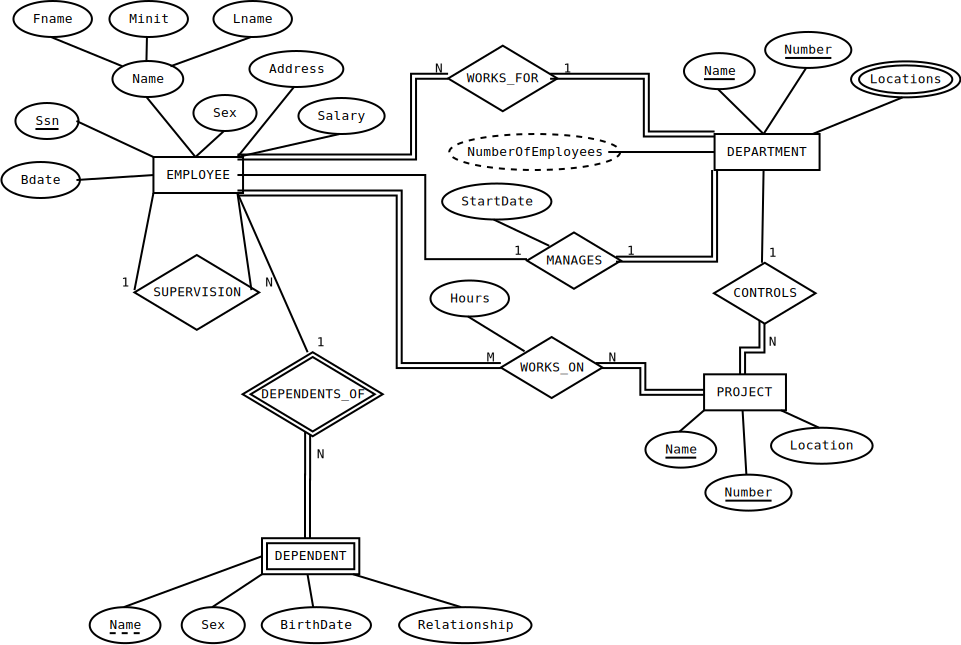
\includegraphics[width=0.6\textwidth]{exemplos/diagramas/ER.jpeg}
    \fonte{Indicar autor original.}
\end{figure}


\begin{figure}
    \centering
    \caption{Exemplo de diagrama - salvo imagem vetorizada - EPS}
    \label{fig:uml_dia_vetorizado_eps}
	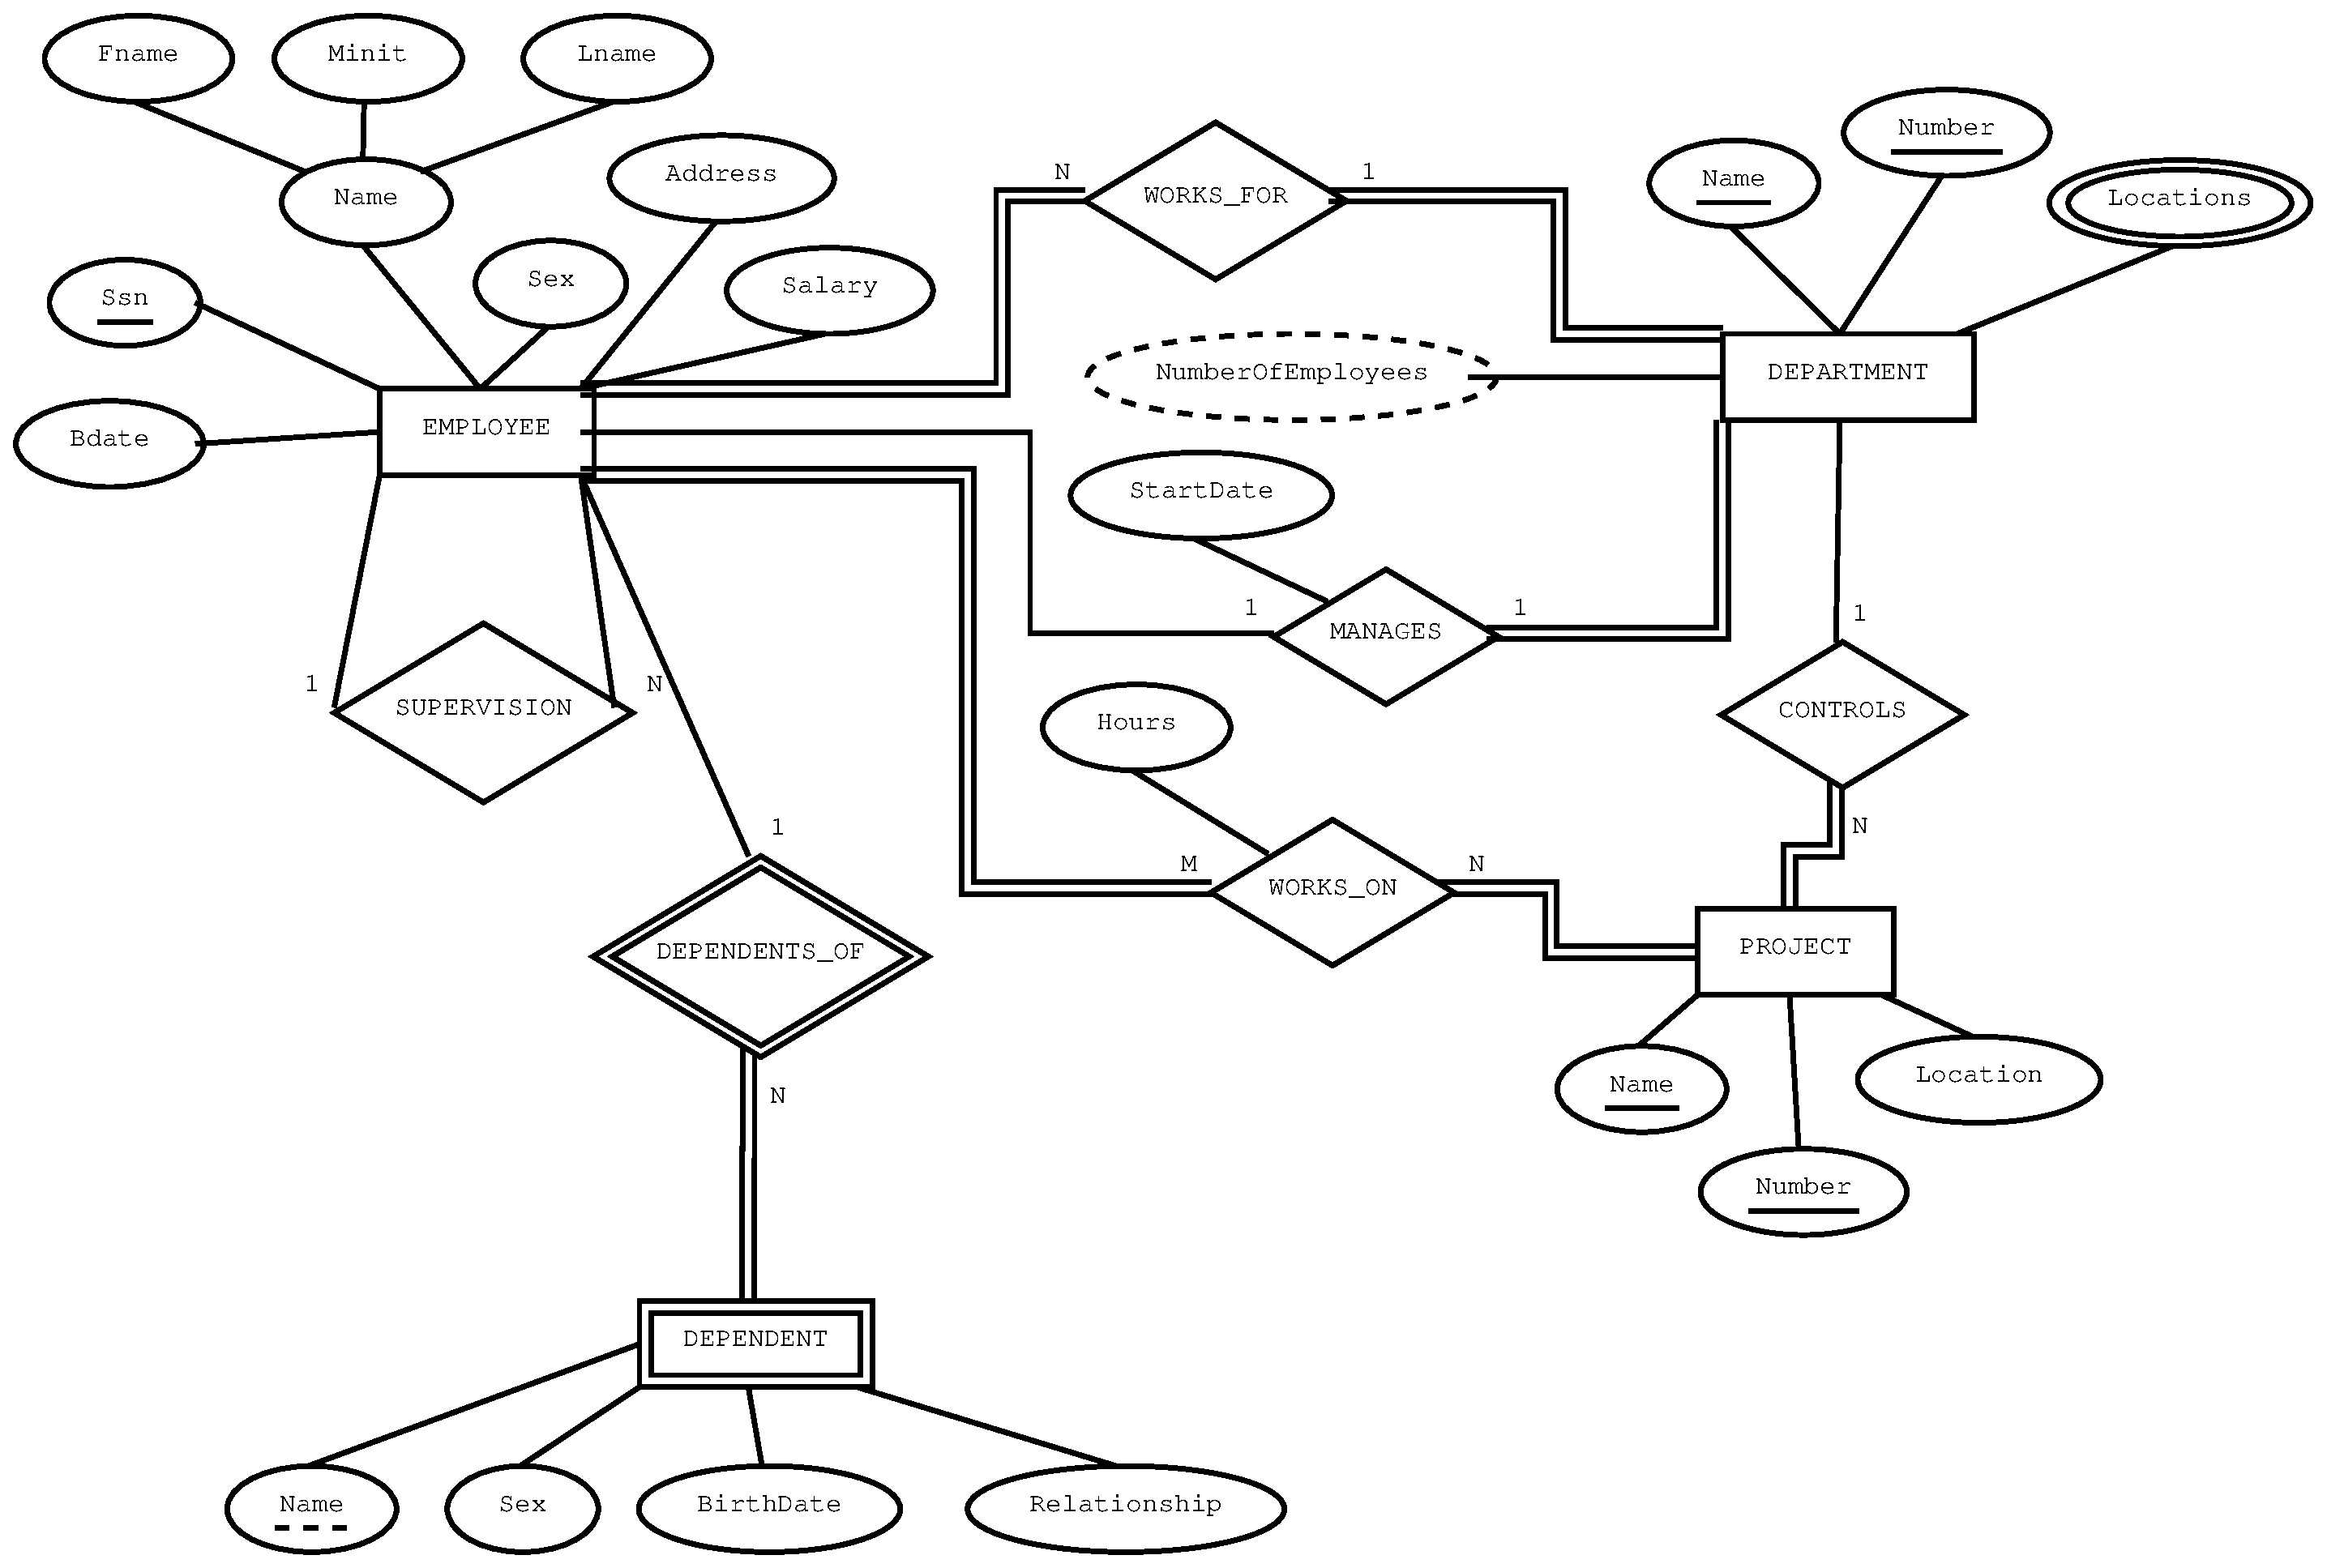
\includegraphics[width=0.6\textwidth]{exemplos/diagramas/ER.eps}
    \fonte{Indicar autor original.}
\end{figure}

\begin{figure}
    \centering
    \caption{Exemplo de diagrama - salvo imagem vetorizada - SVG}
    \label{fig:uml_dia_vetorizado_svg}
    \includesvg[inkscapelatex=false,width=0.6\textwidth]{exemplos/diagramas/ER.svg}
    \fonte{Indicar autor original.}
\end{figure}



% generated by Plantuml 7997beta
\definecolor{plantucolor0000}{RGB}{254,254,206}
\definecolor{plantucolor0001}{RGB}{168,0,54}
\definecolor{plantucolor0002}{RGB}{173,209,178}
\definecolor{plantucolor0003}{RGB}{0,0,0}
\definecolor{plantucolor0004}{RGB}{0,0,255}

\begin{figure}[htb]
    \centering
    \caption{\label{diagramauml}Exemplo de Diagrama UML gerado a partir do PlantUML}
\begin{tikzpicture}[yscale=-1]
\draw[color=plantucolor0001,fill=plantucolor0000,line width=1.5pt] (131pt,29pt) rectangle (223pt,90.8359pt);
\draw[color=plantucolor0001,fill=plantucolor0002,line width=1.0pt] (146pt,45pt) ellipse (11pt and 11pt);
\draw[color=black,fill=black] (148.7656pt,40.875pt) ..controls (148.9219pt,40.6563pt) .. (149.1094pt,40.5469pt) ..controls (149.2969pt,40.4375pt) .. (149.5156pt,40.4375pt) ..controls (149.8906pt,40.4375pt) .. (150.125pt,40.6953pt) ..controls (150.3594pt,40.9531pt) .. (150.3594pt,41.5625pt) -- (150.3594pt,43.0156pt) ..controls (150.3594pt,43.625pt) .. (150.125pt,43.8906pt) ..controls (149.8906pt,44.1563pt) .. (149.5156pt,44.1563pt) ..controls (149.1719pt,44.1563pt) .. (148.9688pt,43.9531pt) ..controls (148.7656pt,43.7656pt) .. (148.6563pt,43.25pt) ..controls (148.6094pt,42.8906pt) .. (148.4219pt,42.7031pt) ..controls (148.0938pt,42.3281pt) .. (147.4844pt,42.1094pt) ..controls (146.875pt,41.8906pt) .. (146.25pt,41.8906pt) ..controls (145.4844pt,41.8906pt) .. (144.8516pt,42.2188pt) ..controls (144.2188pt,42.5469pt) .. (143.7266pt,43.2969pt) ..controls (143.2344pt,44.0469pt) .. (143.2344pt,45.0781pt) -- (143.2344pt,46.1719pt) ..controls (143.2344pt,47.4063pt) .. (144.125pt,48.2266pt) ..controls (145.0156pt,49.0469pt) .. (146.6094pt,49.0469pt) ..controls (147.5469pt,49.0469pt) .. (148.2031pt,48.7969pt) ..controls (148.5938pt,48.6406pt) .. (149.0156pt,48.2031pt) ..controls (149.2813pt,47.9375pt) .. (149.4297pt,47.8594pt) ..controls (149.5781pt,47.7813pt) .. (149.7813pt,47.7813pt) ..controls (150.1094pt,47.7813pt) .. (150.3672pt,48.0391pt) ..controls (150.625pt,48.2969pt) .. (150.625pt,48.6406pt) ..controls (150.625pt,48.9844pt) .. (150.2813pt,49.3906pt) ..controls (149.7813pt,49.9688pt) .. (148.9844pt,50.2969pt) ..controls (147.9063pt,50.75pt) .. (146.6094pt,50.75pt) ..controls (145.0938pt,50.75pt) .. (143.8906pt,50.125pt) ..controls (142.9063pt,49.625pt) .. (142.2188pt,48.5547pt) ..controls (141.5313pt,47.4844pt) .. (141.5313pt,46.2031pt) -- (141.5313pt,45.0469pt) ..controls (141.5313pt,43.7188pt) .. (142.1484pt,42.5703pt) ..controls (142.7656pt,41.4219pt) .. (143.8594pt,40.8047pt) ..controls (144.9531pt,40.1875pt) .. (146.1875pt,40.1875pt) ..controls (146.9219pt,40.1875pt) .. (147.5703pt,40.3516pt) ..controls (148.2188pt,40.5156pt) .. (148.7656pt,40.875pt);
\node at (160pt,37.4531pt)[below right]{Subscriber};
\draw[color=plantucolor0001,line width=1.5pt] (132pt,61pt) -- (222pt,61pt);
\node at (137pt,65pt)[below right]{subscriberId};
\draw[color=plantucolor0001,line width=1.5pt] (132pt,82.8359pt) -- (222pt,82.8359pt);
\draw[color=plantucolor0001,fill=plantucolor0000,line width=1.5pt] (31pt,212pt) rectangle (137pt,273.8359pt);
\draw[color=plantucolor0001,fill=plantucolor0002,line width=1.0pt] (46pt,228pt) ellipse (11pt and 11pt);
\draw[color=black,fill=black] (48.7656pt,223.875pt) ..controls (48.9219pt,223.6563pt) .. (49.1094pt,223.5469pt) ..controls (49.2969pt,223.4375pt) .. (49.5156pt,223.4375pt) ..controls (49.8906pt,223.4375pt) .. (50.125pt,223.6953pt) ..controls (50.3594pt,223.9531pt) .. (50.3594pt,224.5625pt) -- (50.3594pt,226.0156pt) ..controls (50.3594pt,226.625pt) .. (50.125pt,226.8906pt) ..controls (49.8906pt,227.1563pt) .. (49.5156pt,227.1563pt) ..controls (49.1719pt,227.1563pt) .. (48.9688pt,226.9531pt) ..controls (48.7656pt,226.7656pt) .. (48.6563pt,226.25pt) ..controls (48.6094pt,225.8906pt) .. (48.4219pt,225.7031pt) ..controls (48.0938pt,225.3281pt) .. (47.4844pt,225.1094pt) ..controls (46.875pt,224.8906pt) .. (46.25pt,224.8906pt) ..controls (45.4844pt,224.8906pt) .. (44.8516pt,225.2188pt) ..controls (44.2188pt,225.5469pt) .. (43.7266pt,226.2969pt) ..controls (43.2344pt,227.0469pt) .. (43.2344pt,228.0781pt) -- (43.2344pt,229.1719pt) ..controls (43.2344pt,230.4063pt) .. (44.125pt,231.2266pt) ..controls (45.0156pt,232.0469pt) .. (46.6094pt,232.0469pt) ..controls (47.5469pt,232.0469pt) .. (48.2031pt,231.7969pt) ..controls (48.5938pt,231.6406pt) .. (49.0156pt,231.2031pt) ..controls (49.2813pt,230.9375pt) .. (49.4297pt,230.8594pt) ..controls (49.5781pt,230.7813pt) .. (49.7813pt,230.7813pt) ..controls (50.1094pt,230.7813pt) .. (50.3672pt,231.0391pt) ..controls (50.625pt,231.2969pt) .. (50.625pt,231.6406pt) ..controls (50.625pt,231.9844pt) .. (50.2813pt,232.3906pt) ..controls (49.7813pt,232.9688pt) .. (48.9844pt,233.2969pt) ..controls (47.9063pt,233.75pt) .. (46.6094pt,233.75pt) ..controls (45.0938pt,233.75pt) .. (43.8906pt,233.125pt) ..controls (42.9063pt,232.625pt) .. (42.2188pt,231.5547pt) ..controls (41.5313pt,230.4844pt) .. (41.5313pt,229.2031pt) -- (41.5313pt,228.0469pt) ..controls (41.5313pt,226.7188pt) .. (42.1484pt,225.5703pt) ..controls (42.7656pt,224.4219pt) .. (43.8594pt,223.8047pt) ..controls (44.9531pt,223.1875pt) .. (46.1875pt,223.1875pt) ..controls (46.9219pt,223.1875pt) .. (47.5703pt,223.3516pt) ..controls (48.2188pt,223.5156pt) .. (48.7656pt,223.875pt);
\node at (60pt,220.4531pt)[below right]{AccumUsage};
\draw[color=plantucolor0001,line width=1.5pt] (32pt,244pt) -- (136pt,244pt);
\node at (37pt,248pt)[below right]{subscriberId};
\draw[color=plantucolor0001,line width=1.5pt] (32pt,265.8359pt) -- (136pt,265.8359pt);
\draw[color=plantucolor0001,fill=plantucolor0000,line width=1.5pt] (221pt,191pt) rectangle (318pt,294.3438pt);
\draw[color=plantucolor0001,fill=plantucolor0002,line width=1.0pt] (240.05pt,207pt) ellipse (11pt and 11pt);
\draw[color=black,fill=black] (242.8156pt,202.875pt) ..controls (242.9719pt,202.6563pt) .. (243.1594pt,202.5469pt) ..controls (243.3469pt,202.4375pt) .. (243.5656pt,202.4375pt) ..controls (243.9406pt,202.4375pt) .. (244.175pt,202.6953pt) ..controls (244.4094pt,202.9531pt) .. (244.4094pt,203.5625pt) -- (244.4094pt,205.0156pt) ..controls (244.4094pt,205.625pt) .. (244.175pt,205.8906pt) ..controls (243.9406pt,206.1563pt) .. (243.5656pt,206.1563pt) ..controls (243.2219pt,206.1563pt) .. (243.0188pt,205.9531pt) ..controls (242.8156pt,205.7656pt) .. (242.7063pt,205.25pt) ..controls (242.6594pt,204.8906pt) .. (242.4719pt,204.7031pt) ..controls (242.1438pt,204.3281pt) .. (241.5344pt,204.1094pt) ..controls (240.925pt,203.8906pt) .. (240.3pt,203.8906pt) ..controls (239.5344pt,203.8906pt) .. (238.9016pt,204.2188pt) ..controls (238.2688pt,204.5469pt) .. (237.7766pt,205.2969pt) ..controls (237.2844pt,206.0469pt) .. (237.2844pt,207.0781pt) -- (237.2844pt,208.1719pt) ..controls (237.2844pt,209.4063pt) .. (238.175pt,210.2266pt) ..controls (239.0656pt,211.0469pt) .. (240.6594pt,211.0469pt) ..controls (241.5969pt,211.0469pt) .. (242.2531pt,210.7969pt) ..controls (242.6438pt,210.6406pt) .. (243.0656pt,210.2031pt) ..controls (243.3313pt,209.9375pt) .. (243.4797pt,209.8594pt) ..controls (243.6281pt,209.7813pt) .. (243.8313pt,209.7813pt) ..controls (244.1594pt,209.7813pt) .. (244.4172pt,210.0391pt) ..controls (244.675pt,210.2969pt) .. (244.675pt,210.6406pt) ..controls (244.675pt,210.9844pt) .. (244.3313pt,211.3906pt) ..controls (243.8313pt,211.9688pt) .. (243.0344pt,212.2969pt) ..controls (241.9563pt,212.75pt) .. (240.6594pt,212.75pt) ..controls (239.1438pt,212.75pt) .. (237.9406pt,212.125pt) ..controls (236.9563pt,211.625pt) .. (236.2688pt,210.5547pt) ..controls (235.5813pt,209.4844pt) .. (235.5813pt,208.2031pt) -- (235.5813pt,207.0469pt) ..controls (235.5813pt,205.7188pt) .. (236.1984pt,204.5703pt) ..controls (236.8156pt,203.4219pt) .. (237.9094pt,202.8047pt) ..controls (239.0031pt,202.1875pt) .. (240.2375pt,202.1875pt) ..controls (240.9719pt,202.1875pt) .. (241.6203pt,202.3516pt) ..controls (242.2688pt,202.5156pt) .. (242.8156pt,202.875pt);
\node at (254.95pt,199.4531pt)[below right]{IpSession};
\draw[color=plantucolor0001,line width=1.5pt] (222pt,223pt) -- (317pt,223pt);
\node at (227pt,227pt)[below right]{ipAddress};
\node at (227pt,240.8359pt)[below right]{specificData};
\node at (227pt,254.6719pt)[below right]{sapcOriginStateId};
\node at (227pt,268.5078pt)[below right]{apnId};
\draw[color=plantucolor0001,line width=1.5pt] (222pt,286.3438pt) -- (317pt,286.3438pt);
\draw[color=plantucolor0004] (191.942pt,90.081pt) ..controls (205.204pt,115.893pt) and (224.952pt,154.325pt) .. (241.265pt,186.076pt);
\draw[color=plantucolor0004,fill=plantucolor0004] (243.646pt,190.709pt) -- (243.0894pt,180.8759pt) -- (241.3604pt,186.262pt) -- (235.9742pt,184.5329pt) -- (243.646pt,190.709pt) -- cycle;
\node at (191.0584pt,98.9168pt)[below right]{1};
\node at (230.3817pt,166.6703pt)[below right]{1..*};
\draw[color=plantucolor0001] (162.058pt,90.081pt) ..controls (145.645pt,122.023pt) and (119.302pt,173.295pt) .. (101.824pt,207.31pt);
\draw[color=plantucolor0001,fill=plantucolor0001] (99.5252pt,211.784pt) -- (107.1969pt,205.6078pt) -- (101.8108pt,207.337pt) -- (100.0816pt,201.9509pt) -- (99.5252pt,211.784pt) -- cycle;
\node at (143.0082pt,98.7264pt)[below right]{1};
\node at (101.801pt,187.522pt)[below right]{0..1};
\end{tikzpicture}
	\legend{Fonte: Exemplos PlantUML.}
\end{figure}

A \autoref{fig_diag_virado} exemplifica como utilizar uma imagem em formato paisagem (página inteira). Obs: Utilizamos propositalmente uma imagem não vetorizada de forma a ilustrar o procedimento e também para apresentar que a qualidade não fica boa o suficiente para leitura. Uma versão vetorizada dessa figura teria qualidade melhor.


% observe que a imagem a seguir teve que ser ajustada para caber corretamente na página
% por não ser uma imagem vetorizada a qualidade não é a melhor possivel
\begin{sidewaysfigure}[htb]
    \centering
	\caption{\label{fig_diag_virado}Diagrama Virado - Exemplo}
	\includegraphics[width=0.9\textwidth]{exemplos/exemplo_diag_horizontal.png}
	\fonte{\citeonline{openehrCompositionEntry}.}
\end{sidewaysfigure}


\subsection{Impressão em folhas formato A3}

A página seguinte em A3 permite a impressão de diagramas grandes que não podem ser visualizados facilmente em folha padrão A4. Lembre que algumas impressoras podem ter problemas com isso, então selecione somente as páginas A4 ao imprimir e depois imprima separadamente a página A3.

A \autoref{fig_logo_A3} utiliza a mesma imagem da \autoref{fig_logo} e foi ampliada para demonstrar a essa possibilidade de impressão de grandes imagens em A3.

Observe que o código de exemplo vai gerar uma quebra de página no local onde for definida a página A3, por isso não deve ser utilizado entre textos para evitar grandes espaços em branco.

Folhas impressas em A3 ou tamanhos maiores devem ser dobradas seguindo o padrão definido pela ABNT. 


Cuidado ao utilizar folhas A3 em um documento impresso em frente e verso pois a numeração das páginas seguintes pode ser impressa de forma incorreta (posição do número na página). Uma alternativa para esta situação é manter todas páginas impressas em A3 no último apêndice, fazendo as referencias corretas durante o texto.



\afterpage{%
\begin{PAGINA-A3}

\begin{figure}[p]
    \centering%
    \fcolorbox{red}{yellow}{ \includegraphics[height=\textheight,width=\textwidth,keepaspectratio]{\ifspprefixo/logo-02.jpg}}%
	\caption{\label{fig_logo_A3}Logotipo IFSP em página A3}
	\legend{Com borda para demonstrar os limites}
   \fonte{Autor da Figura}
\end{figure}

\end{PAGINA-A3}
}


%DIF > %
% Macros para simplificar a demonstração dos erros
%

\newcommand{\errado}[1]{\textbf{\textcolor{red}{#1}}}
\newcommand{\certo}[1]{\textbf{\textcolor{ForestGreen}{#1}}}
% Para não confundir com os exemplos de certo e errado não são colocados os pontos e ponto e virgula dos itens
\newcommand{\erradocerto}[3]{\item #1:\begin{itemize}
    \item \errado{#2}
    \item \certo{#3}
\end{itemize}}
\newcommand{\erradoerradocerto}[4]{\item #1:\begin{itemize}
    \item \errado{#2}
    \item \errado{#3}
    \item \certo{#4}
\end{itemize}}
\newcommand{\erradocertocerto}[4]{\item #1:\begin{itemize}
    \item \errado{#2}
    \item \certo{#3}
    \item \certo{#4}
\end{itemize}}



% Para demonstrar o erro nome deve ser igual entre o capitulo e a seção, então fica em um comando para facilitar
\newcommand{\nomeDoCapitulo}{Erros comuns em documentos}
\chapter{\nomeDoCapitulo}
\label{erros-comuns-capitulo}

% Não colocar nada aqui pois é uma demonstração de erro comum
\explicacaoErro{Passando de capítulo para seção sem texto}
\explicacaoErro{Seção com mesmo nome do capítulo}

\section{\nomeDoCapitulo}
\label{erros-comuns}

% Não colocar nada aqui pois é uma demonstração de erro comum
\explicacaoErro{Passando de seção para subseção sem texto}

\subsection{Subseção sem texto entre o item anterior}
\label{erros-comuns-sub1}


% Tem um erro proposital aqui duplicando "seção" que é escrita também pelo autoref, esse erro é citado em um paragrafo na sequencia....
Essa seção \autoref{erros-comuns} demonstra alguns dos erros mais comuns que percebemos em trabalhos de alunos. Alguns itens errados são apresentados em \errado{vermelho} e corretos em \certo{verde}, mas devido a formatação dos links pode haver uma variação. Lembre que a utilização de cores não é recomendada no documento acadêmico, elas foram utilizadas nesse documento para facilitar a demonstração dos erros.

Além desses erros é comum encontrar a falta de correção ortográfica e utilização errada de palavras. É importante sempre utilizar a correção ortográfica e ainda fazer a revisão por diversas pessoas para evitar erros de português, a língua portuguesa tem palavras parecidas com sentidos diferente, cuidado com a utilização dos acentos e pontuação como pode ser visto claramente em  \autoref{fig_portugues_amador}.

No \autoref{revisao-de-textos} é apresentado um processo simples para revisão de documentos que detecta a maior parte dos erros descritos neste documento.

% erro proposital que esta no inicio da seção
Você percebeu que essa seção iniciou com um erro e que esse erro não está indicado em vermelho ?


\begin{figure}[htb]
    \centering
	\caption{\label{fig_portugues_amador}Português não é para amador}
	\frame{\includegraphics[width=0.9\textwidth]{erros/portugues_nao_eh_para_amador.jpg}}
	\fonte{Autor Desconhecido.}
\end{figure}


Exemplos de erros encontrados em documentos das disciplinas de projetos são apresentados nas seções seguintes. E existem dicas adicionais sobre textos disponíveis em \url{https://dicas.ivanfm.com/aulas/textos/}.


\todo[inline]{Separar esses itens em grupos mais específicos}

\subsection{Subseção com titulo que tenta ser introdução:}
\label{erros-titulo-dois-pontos}
\errado{Colocar um título de seção/seção com dois pontos no final tentando indicar uma introdução para o texto da seção.}
\explicacaoErro{Além disso essa seção tem somente um pequeno parágrafo, ver \autoref{erros-formatacao-docto}}

\subsection{Erros comuns de texto}
    
\begin{itemize}
    \erradocerto{Abreviação ou nomes incompletos dos participantes do trabalho e/ou professores na capa do documento}{Cebolácio Silva}{Cebolácio Júnior Menezes da Silva}

    \erradocerto{Falta de prontuário completo do estudante na capa do documento }{Magali Fernandes de Lima   123456}{Magali Fernandes de Lima    SP123456}

    \item cada parágrafo deve descrever uma ideia então cuidado ao escrever um parágrafo grande demais com diversas ideias envolvidas ou escrever diversos parágrafos pequenos para a mesma ideia; 
        
    \erradocerto{não utilizar palavras em português onde for possível}{o dispositivo mobile}{o dispositivo móvel}

    \erradocerto{não utilizar melhores palavras, algumas palavras chegaram a ser incorporadas a língua portuguesa mas existem palavras melhores e que podem ser utilizadas e as vezes com resultado mais claro}{postagem / deletar / customizar}{publicação / excluir / personalizar}

    \erradocerto{Utilização do tempo verbal incorreto, a escrita do documento muitas vezes inicia antes da finalização, mas o leitor recebe o documento depois do trabalho finalizado}{será desenvolvido - será apresentado}{foi desenvolvido - é apresentado}

    \erradoerradocerto{Referenciar elementos indicando posição, acima, abaixo, a seguir }{... como poder ser visto na Figura abaixo ...}{... como pode ser visto no quadro a seguir ....}{... como pode ser visto na \autoref{fig_portugues_amador} ...}

    \erradocerto{não representar as unidades de forma correta}{3,20 ghz}{3,20 GHz}

    \erradocerto{não ser consistente com os formatos e precisões}{o primeiro tem \textit{clock} de 3,20 GHz e o segundo de 1,8 GHz}{o primeiro tem \textit{clock} de 3,20 GHz e o segundo de 1,80 GHz}
        
    \erradocerto{Escrever as mesmas palavras, com o mesmo sentido de diversas formas diferentes. Um exemplo é o nome de uma empresa famosa em alguns desenhos: ACME}{ACME Corporation é uma sociedade fictícia que existe no universo dos filmes e animações \newline ... \newline A companhia acme reapareceu num desenho animado do Hortelino Troca-Letras com um kit para aprender boxe por correspondência \newline ... \newline Os produtos Acme podem ser encomendados somente pelo correio}{ACME Corporation é uma sociedade fictícia que existe no universo dos filmes e animações \newline ... \newline A companhia ACME reapareceu num desenho animado do Hortelino Troca-Letras com um kit para aprender boxe por correspondência \newline ... \newline Os produtos ACME podem ser encomendados somente pelo correio}
    
\end{itemize}

\subsection{Erros comuns relacionados a formatação do texto e do documento}
\label{erros-formatacao-docto}

\begin{itemize}
    \item \errado{passagem de um item para outro sem texto} como é possível observar entre  \autoref{erros-comuns-capitulo} e \autoref{erros-comuns} e também entre \autoref{erros-comuns} e \autoref{erros-comuns-sub1};
    
    \item \errado{itens com pouco texto} observe que as seções 
    \ref{erros-titulo-dois-pontos}, \ref{erros-comuns-sub-pequena1} e a \ref{erros-comuns-sub-pequena2} possuem pouco texto, cada item deve ter um volume de texto que justifique sua existência, caso o volume de texto seja pequeno agrupe as seções em uma única seção com mais parágrafos;
        
    \item \errado{utilizar o mesmo nome para seções / capítulos como \autoref{erros-comuns-capitulo} e \autoref{erros-comuns}};
        
    \item definições de referências incompletas, a referência \citeonline{ETAL4} está definida faltando cidade, observe que na lista de referencias aparece \errado{[S.l.]} que indica Sem Local, pois a \ac{abnt} exige a indicação de local para livros;

    \erradocerto{incluir dentro do seu texto um documento ou manual que pode ser referenciado e facilmente acessado pelo leitor, faça a citação correta referenciando o documento original}{segundo a \ac{ldb}, a educação brasileira é dividida em dois níveis: a educação básica e o ensino superior}{segundo a \ac{ldb} 9394/96 \cite{ldb}, a educação brasileira é dividida em dois níveis: a educação básica e o ensino superior}
    
    \erradocerto{citação de elementos errados}{Segundo o anexo com o manual pdfpages (\autoref{manual-todonotes}), o comando \mostraComandoLaTeX{includepdf} permite que você faça a inclusão de páginas de documentos externos no seu documento}{Segundo o anexo com o manual pdfpages (\autoref{manual-pdfpages}), o comando \mostraComandoLaTeX{includepdf} permite que você faça a inclusão de páginas de documentos externos no seu documento}
    
    \item \errado{forçar manualmente quebra de página}, o texto deve seguir utilizando todo o espaço disponível nas páginas, o {\LaTeX} faz isso automaticamente, não é necessário forçar uma quebra de página;
    
    \item \errado{não seguir as dicas de revisão} - ver \autoref{revisao-de-textos};
    
    \item \errado{não formatar corretamente tabelas} como indicado na \autoref{sub-erros-tabelas}.

    
\end{itemize}





\subsection{Erros comuns no uso do \LaTeX}

O \LaTeX\ é uma linguagem onde você define o texto e comandos e o resultado da compilação é um arquivo formatado normalmente no formato \ac{pdf}. Com isso algumas características dessa linguagem devem ser consideradas ao escrever seu texto para não cair em alguns problemas já conhecidos:

\begin{itemize}
    \erradocerto{ignorar que após uma macro pode ser necessário incluir um espaço forçado (observe pelo código fonte as diversas maneiras utilizadas para fazer corretamente)}{o \LaTeX permite...}{o \LaTeX\ permite...\newline o {\LaTeX} permite...\newline o \LaTeX \space permite...}

    \erradocertocerto{erro ao definir elementos com aspas, observe que dependendo da forma utilizada o texto fica \enquote{grudado} (observe no código fonte as diferenças)}{"entre aspas" após as aspas}{"entre aspas" \space após as aspas}{\enquote{entre aspas} após as aspas}

    \erradocerto{não utilizar o sistema de siglas / glossário para definições especificas (as definições corretas ficam como links no arquivo final \acs{pdf}), ver \autoref{siglas-glossario}}{IFSP}{\acs{ifsp}}
    
    \erradocerto{Não utilizar a definição de plural do glossário e fazer um plural manualmente}{\gls{crud}s - utilizando a sigla seguida do s para plural}{\glspl{crud} utilizando a definição de plural do glossário}
    
\end{itemize}


\subsection{Subseção com texto pequeno 1}
\label{erros-comuns-sub-pequena1}
\errado{Uma frase única indicando basicamente o que o título da seção é}.

\subsection{Subseção com texto pequeno 2}
\label{erros-comuns-sub-pequena2}
\errado{Mais um paragrafo único indicando basicamente o que o título da seção é, provavelmente isso poderia ir para o glossário, ver \autoref{siglas-glossario}}, uma regra simples para seguir é \certo{se uma seção não tiver pelo menos 3 (três) parágrafos, provavelmente essa informação não precisa de uma seção especifica e pode fazer parte de outra seção}

\subsection{Erros no uso de Ilustrações}
\label{sub-erros-ilustrações}

Ilustrações são elementos não textuais que ajudam na apresentação de informação como Figuras, Quadros e Tabelas.


\begin{itemize}

    \item \errado{utilização de páginas em formato paisagem ou em formato A3 sem necessidade}, antes de fazer isso tente reorganizar as ilustrações para caberem na página no formato padrão (ex um quadro que tem muitas colunas, pode ser alterado para que as colunas virem linhas e dessa forma caber na página em formato padrão);
    
    \erradocerto{não referenciar uma ilustração no texto, toda ilustração deve ser referenciada no texto}{(...)parecidas com sentidos diferente, cuidado com a utilização dos acentos e pontuação como pode ser visto abaixo.}{(...)parecidas com sentidos diferente, cuidado com a utilização dos acentos e pontuação como pode ser visto claramente em \autoref{fig_portugues_amador}}
    
    \erradocerto{não referenciar ilustrações da forma correta, observe que não é somente a questão de maiúscula/minúscula mas também o link que inclui o tipo de ilustração}{a tabela \ref{tabela-correta-equipamento} ...}{a \autoref{tabela-correta-equipamento} ...}
    
    \erradoerradocerto{não referenciar corretamente sequencias de ilustrações, esse caso pode até dar a impressão de inconsistência com o caso anterior}{nas \autoref{tab-exemplo} até \autoref{tabela-correta-servicos}}{nas Tabelas de  \autoref{tab-exemplo} até \autoref{tabela-correta-servicos}}{nas Tabelas de \ref{tab-exemplo} até \ref{tabela-correta-servicos} \newline a partir da \autoref{tab-exemplo} até a \autoref{tabela-correta-servicos}}

    \erradocerto{deixar referencia jogada sem fazer parte do texto}{durante o projeto foram registradas as métricas. \autoref{tabela-correta-servicos}}{a \autoref{tabela-correta-servicos} apresenta os valores das métricas levantadas durante o projeto.}

    \item \errado{\enquote{estourar} a margem do documento, como na \autoref{tabela-errada}};
    
    \erradoerradocerto{indicar a ferramenta utilizada como fonte de ilustração}{Fonte: Trello}{Fonte: Excel}{Fonte: Os Autores}
    
    \item \errado{repetir a mesma ilustração em dois locais no documento, a figura não deve ser repetida, mas referenciada novamente};

    \item \errado{não utilizar imagens vetorizadas} para obter a melhor qualidade, ver \autoref{sec_figuras};

    \item \errado{utilização de cores em um documento que vai ser impresso em preto e branco};

    \item \errado{tentar posicionar ilustrações em locais específicos} (ex abaixo do texto), o correto é referenciar a ilustração no texto e deixar o \LaTeX\ posicionar de acordo com a disponibilidade de espaço no documento, mas você deve recomendar que o local da definição seja prioritário, ver \autoref{elementos-nao-textuais}. Se as suas imagens ficam distantes do texto onde foram referenciadas provavelmente você não descreveu de forma suficiente as ilustrações ou você precisa de mais texto condizente no seu documento;
    
    \item \errado{ilustrações muito distantes do local onde foram citadas}, o {\LaTeX} ajusta o posicionamento das ilustrações automaticamente, você deve colocar a definição próximo do local da citação e não ficar forçando quebras de páginas. Se suas ilustrações estão ficando longe da referencia significa que você tem pouco texto e com isso as ilustrações ficam distantes. Em alguns casos uma opção pode ser utilizar os apêndices para conjuntos grandes de ilustrações deixando o texto principal mais organizado, além disso esse modelo possui um comando \mostraComandoLaTeX{autorefWithPage} que pode auxiliar em alguns casos onde for necessário referenciar uma ilustração que fique posicionada distante do local de citação.
\end{itemize}

Os nomes que definimos para as ilustrações devem ser claros o bastante para permitir que o leitor os identifique nas listas no inicio do documento. A \autoref{fig_erros_lista_quadros} apresenta um trecho de uma lista de quadros com dois problemas encontrados em trabalhos :

\begin{itemize}
    \erradocerto{Repetição de nomes em elementos diferentes}{é possível observar que existem dois quadros com nome \textbf{Caso de Uso 10} na \autoref{fig_erros_lista_quadros}}{Cada elemento deve ter um nome próprio}

    \erradocerto{Utilização de nomes que não são claros para cada elemento}{Caso de Uso 07}{Caso de Uso 07 - Recuperação de senha}.
    
    \erradocerto{Nomes que não indicam claramente o conteúdo da ilustração como é possível observar na \autoref{fig_erros_lista_quadros_2}}{Quadro X - Usuário}{Quadro X - Dicionário de dados - Entidade Usuário}
\end{itemize}


\begin{figure}[htb]
    \centering
	\caption{\label{fig_erros_lista_quadros}Exemplo de Lista de quadros com erros comuns (Casos de uso)}
	\frame{\includegraphics[width=0.9\textwidth]{erros/erros_lista_quadros.png}}
    \fonte{Trecho de um trabalho com o erro (omitida autoria propositadamente).}
\end{figure}

\begin{figure}[htb]
    \centering
	\caption{\label{fig_erros_lista_quadros_2}Exemplo de Lista de quadros com erro nos títulos}
	\frame{\includegraphics{erros/quadros_login_usuario.png}}
    \fonte{Trecho de um trabalho com o erro (omitida autoria propositadamente).}
\end{figure}



\subsection{Erros em tabelas e quadros}
\label{sub-erros-tabelas}
A \autoref{tabelas-e-quadros} demonstra como devemos formatar corretamente tabelas e quadros (e também indica quando devemos utilizar cada tipo de ilustração), a \autoref{tabela-errada} mostra diversos erros comuns que encontramos em tabelas e quadros, e as Tabelas \ref{tabela-correta-equipamento} e \ref{tabela-correta-servicos} mostram os mesmos dados apresentados de uma forma correta. Uma tabela formatada corretamente permite a leitura e comparação dos dados de forma mais fácil. Observe a lista de erros da \autoref{tabela-errada} :


\begin{itemize}
    \item \errado{formatação de bordas como um quadro e não como tabela};

    \item \errado{títulos sem negrito dificultando a sua leitura e identificação};
    
    \item \errado{não limitar tamanho de coluna que tem dados grandes de forma a estourar o espaço disponível};
    
    \item \errado{números não estão alinhados a direita};
    
    \item \errado{itens sem ordem especifica}, \certo{os itens devem vir em uma ordem lógica ou ordem alfabética};
    
    \item \errado{inconsistência de precisão, em uma célula o valor tem duas casas decimais e em outras não possuem casas decimais};
    
    \item \errado{mistura de dados de situações diferentes (ex: custo único e custo mensal sem normalização)};
    
    \item \errado{repetição do R\$ mesmo tendo ele no título da coluna}.
\end{itemize}

% Essa tabela além dos erros na colocação dos dados também está "estourando" a margem pois não está quebrando o texto um caso muito comum nos documentos que recebemos... 
\begin{table}[thb]
\centering
\ABNTEXfontereduzida
\caption{Valores de equipamentos (formação de forma errada e passando da margem)}
\label{tabela-errada}
\begin{tabular}{|l|c|l|l|}
\hline
Equipamento/Serviço & Valor Unitário R\$ & Quantidade & Valor Total R\$ \\ \hline
Teclado     & R\$60          & 2          & R\$120     \\ \hline
Monitor     & R\$:600          & 2          & R\$ 1200,00     \\ \hline
Internet     & R\$220          & 1          & R\$ 220     \\ \hline
Texto muito muito grande que deveria ser quebrado   & R\$120          & 1          & R\$ 120     \\ \hline
\end{tabular}
	\fonte{Os Autores.}
\end{table}

\begin{table}[]
\centering
\ABNTEXfontereduzida
\caption{Valores de equipamentos - Compra (formatada corretamente)}
\label{tabela-correta-equipamento}
\begin{tabular}{p{5.0cm}rrr}
\hline
\thead{Equipamento} & \thead{Valor\\Unitário\\R\$} & \thead{Quantidade} & \thead{Valor\\Total\\ R\$} \\ \hline
Monitor     & 600,00          & 2          & 1200,00     \\ 
Teclado     & 60,00          & 2          & 120,00     \\ 
Texto muito muito grande que deveria ser quebrado     & 220,00          & 1          & 220,00     \\ 
\hline
\textbf{TOTAL} & & & 1540,00 \\
\hline
\end{tabular}
\fonte{Os autores.}
\end{table}

\begin{table}[]
\centering
\ABNTEXfontereduzida
\caption{Valores de equipamentos - Mensal (formatada corretamente)}
\label{tabela-correta-servicos}
\begin{tabular}{lrrr}
\hline
\thead{Serviço} & \thead{Valor Unitário R\$} & \thead{Quantidade} & \thead{Valor Mensal R\$} \\ \hline
Internet     & 120,00          & 1          & 120,00     \\ \hline
\end{tabular}
\fonte{Os autores.}
\end{table}

Também é necessário cuidado em termos de formatação das ilustrações em termos de consistência e quebras :

\begin{itemize}
    
    \item \errado{quadros que devem representar o mesmo tipo de informação com formatação diferente}, uma maneira simples de garantir a padronização da formatação é utilizar o recurso de criação de comandos no {\LaTeX}, dessa forma todos elementos serão apresentados de forma consistente;

    \item \errado{utilização de \index{longtable}longtable sem necessidade} quebrando um quadro ou tabela que poderia ser apresentado em uma única página, quando o quadro ou tabela for maior que uma página a melhor maneira é quebrar em quadros que agrupem as informações de forma consistente.

\end{itemize}

\todo[inline]{gerar figura demonstrando erro do longtable com tabelas pequenas que ficam quebradas em diferentes páginas}    


Em quadros pequenos detalhes podem fazer uma grande diferença na apresentação de informação, como pode ser observado nos Quadros \ref{quadro-poluido},  \ref{quadro-poluido-limpo-desalinhado} e \ref{quadro-poluido-limpo} :

\begin{itemize}
    \item \errado{O \autoref{quadro-poluido} foi montado com textos que não facilitam a leitura};
    
    \item \errado{O \autoref{quadro-poluido-limpo-desalinhado} teve uma melhora mas sem centralização das informações};

    \item \certo{O \autoref{quadro-poluido-limpo} apresenta a mesma informação do de forma mais limpa e facilitando a leitura}.
\end{itemize}



\begin{quadro}[thb]
\centering
\ABNTEXfontereduzida
\caption{Distribuição de Atividades (poluído, difícil de ler) }
\label{quadro-poluido}
\begin{tabular}{|l|c|c|c|c|}
\hline
\thead{Responsável} & \thead{Atividade 1} & \thead{Atividade 2} & \thead{Atividade 3} & \thead{Atividade 4} \\
\hline
%
Pessoa 1 & SIM         & NÃO         & NÃO         & SIM         \\
\hline
Pessoa 2 & SIM         & NÃO         & SIM         & NÃO         \\
\hline
Pessoa 3 & NÃO         & SIM         & NÃO         & NÃO         \\
\hline
Pessoa 4 & NÃO         & SIM         & SIM         & NÃO        \\
\hline
\end{tabular}
\fonte{Os autores.}
\end{quadro}


\begin{quadro}[thb]
\centering
\ABNTEXfontereduzida
\caption{Distribuição de Atividades (sem centralização)}
\label{quadro-poluido-limpo-desalinhado}
\begin{tabular}{|l|l|l|l|l|}
\hline
\thead{Responsável} & \thead{Atividade 1} & \thead{Atividade 2} & \thead{Atividade 3} & \thead{Atividade 4} \\
\hline
Pessoa 1 & \circlemark       &          &             & \circlemark         \\
\hline
Pessoa 2 & \circlemark       &          & \circlemark      &          \\
\hline
Pessoa 3 &          & \circlemark         &             &          \\
\hline
Pessoa 4 &          & \circlemark         & \circlemark      &         \\
\hline
\end{tabular}
\fonte{Os autores.}
\end{quadro}


\begin{quadro}[thb]
\centering
\ABNTEXfontereduzida
\caption{Distribuição de atividades (de maneira mais clara e simples)}
\label{quadro-poluido-limpo}
\begin{tabular}{|l|c|c|c|c|}
\hline
\thead{Responsável} & \thead{Atividade 1} & \thead{Atividade 2} & \thead{Atividade 3} & \thead{Atividade 4} \\
\hline
Pessoa 1 & \circlemark       &          &             & \circlemark         \\
\hline
Pessoa 2 & \circlemark       &          & \circlemark      &          \\
\hline
Pessoa 3 &          & \circlemark         &             &          \\
\hline
Pessoa 4 &          & \circlemark         & \circlemark      &         \\
\hline
\end{tabular}
\fonte{Os autores.}
\end{quadro}


Utilizar corretamente a área do documento também pode fazer uma grande diferença em termos de espaço. O \autoref{quadro-descritivo-ruim} mostra que se não utilizarmos a área completa de impressão o quadro fica muito grande e difícil de ser posicionado. Os mesmos dados são apresentados no \autoref{quadro-descritivo-melhorado}, utilizando somente o tamanho necessário para os dados e títulos.


\todo[inline]{Completar o texto com mais informações sobre formatação dos quadros}
\begin{quadro}[thb]
\centering
\ABNTEXfontereduzida
\caption{Detalhamento dos itens (ruim)}
\label{quadro-descritivo-ruim}
\begin{tabular}{ | l | p{5.5cm} | l | }
\hline
\thead{Identificador pequeno} & \thead{Descrição} & \thead{Referencia} \\
\hline
XX01 & \lipsum[1]  & ZZ01  \\
\hline
XX02  & bla bla bla & KK02  \\
\hline
XX03 &  bla bla bla & MM03  \\
\hline
\end{tabular}
\fonte{Os autores.}
\end{quadro}


\begin{quadro}[thb]
\centering
\ABNTEXfontereduzida
\caption{Detalhamento dos itens (melhorado)}
\label{quadro-descritivo-melhorado}
\begin{tabular}{ | l | p{12.0cm} | l | }
\hline
\thead{Ident. \\
pequeno} & \thead{Descrição} & \thead{Ref.} \\
\hline
XX01 & \lipsum[1]  & ZZ01  \\
\hline
XX02  & bla bla bla & KK02  \\
\hline
XX03 &  bla bla bla & MM03  \\
\hline
\end{tabular}
\fonte{Os autores.}
\end{quadro}




\subsection{Erros na utilização de referencias}
\label{erros-referencias}

Um trabalho acadêmico deve ser baseado em informações confiáveis, artigos acadêmicos e livros são uma boa fonte de informações confiáveis pois passam por um processo de validação por especialistas antes de sua publicação. Os alunos do \ac{ifsp} tem acesso a diversos livros pela biblioteca online da Editora  Pearson (acessível a partir do \ac{suap}) e também ao serviço de periódicos da \ac{capes} \footnote{\url{http://periodicos.capes.gov.br/}} utilizando a opção \enquote{Acesso CAFE}.

Sempre que possível deve ser utilizada uma referencias primária, ou seja a referencia original da informação, somente quando existir a impossibilidade de acesso a obra original ou a obra original é disponibilizada em uma língua que não seja possível de ler que devemos utilizar as referencias secundárias.

Em alguns casos uma referencia utilizando endereço web pode ser necessária, nesse caso é recomendável manter essas referencias via  Web Archive, de forma a garantir que o leitor tenha acesso ao estado original da referencia utilizada, já que a maioria dos sites normalmente não armazenam histórico de alterações e também alguns sites desaparecem entre a entrega do seu trabalho e a leitura por outras pessoas.

Utilizando o {\LaTeX} parte do processo de tratamento das referencias é simplificado utilizando o padrão bibtex que é disponibilizado em diversas ferramentas, mas a \ac{abnt} possui definições que não são obrigatórias em outros países o que faz com que as referencias precisem de alguns ajustes.


\begin{itemize}
    \erradocerto{utilizar o formato de citação errada em fontes, ver \autoref{referencias}}{Fonte: \cite{alcarde1996}.}{Fonte: \citeonline{alcarde1996}.}

    \erradocerto{Erro na definição de publicações de organizações/empresas (ver definições de NBR6028 no arquivo .bib)}{sem utilizar \textbf{\textit{organization}} \cite{NBR6028:2003-errado}}{utilizando \textbf{\textit{organization}} \cite{NBR6028:2003}}

    \erradocerto{Erro na definição de nomes com acentuação}{...texto \cite{acentuacao-ok}.}{...texto \cite{acentuacao-errada}.}
    
\IfPackageLoaded{biblatex}{%
\explicacaoErro{O erro referente a erro de acentuação só pode ser demonstrado quando o documento foi compilado com \mostraPacoteLaTeX{abntex2cite} e este documento foi compilado com \mostraPacoteLaTeX{biblatex}}
}{}
\end{itemize}



\subsection{Erros em citações indiretas}
\label{erros-citacoes-indiretas}

As citações devem ficar em formato compatível com o texto onde ela estão localizadas. O tipo de citação deve ser escolhido corretamente para isso. O tipo de citação mais utilizado é a citação indireta, onde o o texto é escrito com suas próprias palavras e a referencia indicada.

Utilizar o texto de outra pessoa sem a citação da forma correta é  considerado plágio.

\todo[inline]{informações sobre plágio :  \url{https://dicas.ivanfm.com/aulas/textos/plagio.html}}



O formato deve ser escolhido de acordo com o contexto utilizado :

\begin{itemize}
    \erradoerradocerto{utilizar o formato de citação errada, ver \autoref{referencias}}{de acordo com \cite{alcarde1996} ...}{de acordo com \citeauthor{alcarde1996} ...}{de acordo com \citeonline{alcarde1996}...}

% NBR 10520:2002 ver exemplos em 6.1.5
    \erradoerradocerto{erro ao citar em final do paragrafo, o ponto final fica após a citação }{...texto.\cite{alcione1988} Texto}{\cite{alcione1988} Texto.....}{...texto \cite{alcione1988}. Texto....}


\end{itemize}


\subsection{Erros em citações diretas}
\label{erros-citacoes-diretas}

A \ac{abnt} define formatos específicos para citações diretas (aquelas onde é necessário colocar exatamente o que foi escrito pelo autor referenciado), citações curtas e citações longas (mais de 3 linhas). A citação curta é feita diretamente durante a escrita do texto, mas a citação longa deve ser feita de uma forma especifica. A \autoref{fig_citacao_longa_errada} demonstra a forma errada da citação e a \autoref{fig_citacao_longa_certa} mostra o formato correto para a citação longa.

É importante dar preferencias para citação indireta onde você escreve com suas próprias palavras e indica a fonte da informação. Somente em casos onde o texto original precisa ser utilizado que a citação direta deve ser utilizada.

\begin{figure}[hbt]
    \centering
    \caption{Citação direta longa - incorreta}
    \label{fig_citacao_longa_errada}
\fbox{\begin{minipage}{\textwidth}
Podemos observar que historicamente existem problemas que devem ser tratados: 
    ``\textoFalso{Simulação de Citação}{5}'' \cite{ETAL5}.
\end{minipage}}
\fonte{Os Autores.}
\end{figure}

\begin{figure}[htb]
    \centering
    \caption{Citação direta longa - correta}
    \label{fig_citacao_longa_certa}
    \fbox{\begin{minipage}{\textwidth}
Podemos observar que historicamente existem problemas que devem ser tratados: 
    \begin{citacao}
    \textoFalso{Simulação de Citação}{5} \cite{ETAL5}
    \end{citacao}
\end{minipage}}
\fonte{Os Autores.}
\end{figure}


\subsection{Erros em Apêndices e Anexos}
\label{erros-apendices-e-anexos}

Apesar de parecidos Apêndices e Anexos tem características diferentes. Como Apêndices são colocados documentos adicionais do autor e como Anexos documentos gerados por outras pessoas ou instituições. Mas é necessário cuidado ao escolher o que será colocado nessas áreas do trabalho. Elementos como leis e outros documentos que podem ser facilmente encontrados não devem ser incluídos, mas referenciados (principalmente utilizando a ferramenta \url{https://web.archive.org} que permite salvar a situação de um endereço web em um momento especifico).  


%DIF > \newcommand{\video}[2]{\href{#1}{Vídeo: #2}}

% Erros que serão repetidos/reutilizados em mais de um local
\newcommand{\erroArmazenarSenhaAberta}[0]{armazenamento de senhas abertas (ou com criptografia reversível) no banco de dados sem \textit{hash} \cite{password_storage_cheat_sheet}}    



\chapter{Erros comuns em projetos}
\label{erros-projetos}

Nesse capítulo estão apresentados os erros mais comuns que os professores observam nos sistemas desenvolvidos nas disciplinas de projetos. Alguns fazem parte de mais de uma categoria, mas foram listados cada um em uma categoria representada pela seção do documento.

São apresentados alguns problemas de projeto / modelagem e outros específicos do desenvolvimento.

Algumas referencias indicadas nesse capítulo são de publicações e vídeos disponíveis na internet que devem ser lidas / assistidos para correta compreensão do contexto.

O formato desse capítulo não segue exatamente o formato de documento indicado para os trabalhos acadêmicos.

\todo[inline]{Colocar aqui os erros mais comuns nos projetos de software das disciplinas}

\section{Erros relacionados a Arquitetura / Provedor de serviços}

Cada projeto deve buscar uma arquitetura compatível com seus objetivos, tanto em termos de capacidade como em termos de custos. A escolha do provedor de serviços deve ser feita com cuidado, considerando custos, conhecimentos da equipe e funcionalidades oferecidas. As maquinas devem ser dimensionadas corretamente de forma que não existam grandes custos.

Alguns ambientes oferecem serviços de forma gratuita sem cartão de crédito e outros solicitam forma de pagamento. Nos provedores de serviços com custos variáveis é importante fazer acompanhamento diário do uso e dos custos e escolher corretamente os serviços que são contratados. Utilizar os serviços no sistema aberto em vez das opções acadêmicas/gratuitas pode ser mais simples mas resultar em custos indesejados. 

As escolhas dos serviços devem considerar a real necessidade de uso de forma a ter um uso racional dos recursos. Mesmo um serviço disponibilizado de forma gratuita tem um custo para o provedor e consome energia para funcionar. O abuso no uso dos serviços oferecidos pode gerar limitações futuras e consumir recursos energéticos sem necessidade.

Muitos detalhes que devem ser pensados na definição de arquitetura são apresentados por \citeauthoronline{como_fazer_ingresso_com_escalar} no video \citetitle{como_fazer_ingresso_com_escalar}, esses detalhes vão garantir eficiência no uso de recursos e ainda atender corretamente o usuário da aplicação. Apesar desse vídeo apresentar uma situação que não é tão comum os conceitos se aplicam em praticamente em todos os projetos, saber as possibilidades permite que escolhas corretas sejam feitas.


\section{Erros de Processo}

Os processos da aplicação devem ser desenvolvidos de forma que o usuário possa utilizar a aplicação de maneira simples e intuitiva, existem casos onde o processo atual pode ser redefinido e criar ganhos, mas existem casos onde não é possível redefinir o processo real e o sistema deve atender a esse processo.

Muitas vezes o analista e o desenvolvedor não se colocam no papel do usuário para verificar se o que estão desenvolvendo faz sentido para quem vai realmente utilizar a aplicação. 

\begin{itemize}
    \item interface que não trata o processo de forma simples para o usuário (somente \gls{crud} e o usuário precisa saber qual sequencia deve utilizar);
    
    \item muitas bibliotecas e padrões abertos facilitam o desenvolvimento e simplificam a aplicação, normalmente não existe justificativa para \enquote{reinventar a roda}, ex: 
      \begin{itemize}
          \item utilização de \enquote{login social} OAuth;

          \item utilizações de bibliotecas para tratamentos básicos de segurança;
          
          \item utilizações de bibliotecas para validações;
          
          \item utilização de Gravatar para imagem de perfil.
      \end{itemize}
\end{itemize}

\section{Erros de Segurança}

\begin{itemize}
    \item não seguir recomendações de ferramentas de análise estática e \ac{owasp}, um importante ponto de partida é a leitura de \citetitle{owasp_cheat_sheet};

    \item implementação de um processo de recuperação de senha que depende de dados públicos : 
    Caso real que aconteceu com o sistema do \ac{enem} - \citetitle*{medicina_cachaca}  \cite{medicina_cachaca};

    \item implementação de um processo de autenticação que depende somente de dados públicos - Caso real em setembro/2021 onde um e-commerce utiliza somente CPF e e-mail para \enquote{autenticação} e com esses dados era possível ter acesso a endereço, telefone, bandeira e número final de cartão de crédito e dados dos pedidos. O atendimento do e-commerce informou que não era possível utilizar senha, que o concorrente utilizava o mesmo processo e que os clientes não queriam saber de senha. Ao entrar em contato com a empresa desenvolvedora essa disse que a responsabilidade era da loja que contratou o sistema;
    
    \item utilização de um meio de comunicação que não é seguro para envio de validação em etapa adicional : Caso real de invasão de \gls{telegram} a partir da vulnerabilidade da operadora de telefonia - \citetitle*{invasao_telegram} \citeauthor{invasao_telegram};
    
    \item não fazer validação de e-mail, utilizando \textit{tokens} com validade;
    
    \item armazenamento de credenciais de acesso a banco de dados, servidor de e-mail diretamente dentro de arquivos da aplicação e que são colocados no repositório de controle de versão;
    
    \item não solicitar senha na alteração de dados principais do perfil (e-mail, senha etc);
    
    \item não utilização de parâmetros em \ac{sql} de forma a ficar vulnerável a injeção de \ac{sql} - \autoref{fig:exploits_of_a_mom};

    \item \erroArmazenarSenhaAberta .
\end{itemize}

\begin{figure}
    \centering
    \caption{Vulnerabilidades como injeção de SQL}
	\includegraphics[width=0.95\textwidth]{erros/exploits_of_a_mom.png}
    \fonte{\citeonline{fig_exploits_of_a_mom} / \citeonline{fig_exploits_of_a_mom_explain}.}
    \label{fig:exploits_of_a_mom}
\end{figure}


\section{Erros de modelo de dados}

\begin{itemize}
    \item \erroArmazenarSenhaAberta ;
    
    \item inconsistência na documentação com o método de modelagem utilizado, se a equipe desenvolve a partir de classes utilizando um \ac{orm} que cria as tabelas de forma automática não necessita de um \ac{der}.
    
    \item erro na definição dos modelos apresentados (físico, conceitual, lógico, \ac{der}, \ac{mer}, diagrama de classes);
    
    \item inconsistência entre modelos apresentados (físico, conceitual, lógico, \ac{der}, \ac{mer}, diagrama de classes);

    \item erro na conversão entre modelos;
    
    \item achar que ter um número pequeno de tabelas é mais eficiente que mais tabelas, eficiência tem a ver com modelar corretamente e não com o número de tabelas do banco;
    
    \item dicionário de dados diferente da modelagem apresentada;
    
    \item tipagem de dados incorreta (Ex: um campo para data com tipo VARCHAR);
    
    \item falta de índices adicionais em tabelas do banco de dados, os índices permitem uma busca eficiente sem a leitura completa das tabelas em algumas consultas;
    
    \item falta de teste do modelo definido, muitas vezes não existem campos para armazenamento de informações e também não existem formas de armazenar os dados que se alteram durante o processo e necessitam de histórico;
    
    \item exclusão física de dados que deveriam ser mantidos para histórico;
    
    \item falta de informações para auditoria de processos;
    
    \item erro na escolha de formato de armazenamento de arquivos e imagens (blob ou armazenamento de objetos), cada formato tem vantagens e desvantagens que devem ser considerados de acordo com o contexto da aplicação. Normalmente não faz muito sentido armazenar conteúdos públicos dentro do banco de dados.
    
\end{itemize}

\section{Erros Interface com Usuário}

\begin{itemize}
    \item tradução automática de página via Google tradutor, que acaba gerando falhas de contexto e traduções sem sentido;
    
    \item falta de responsividade em aplicações : web e móvel;
    
    \item não utilizar padrões já existentes para plataforma escolhida;
    
    \item interface complexa para o nível de conhecimento do público alvo da aplicação
    \newline
    \cite{computer_skills}.
    
\end{itemize}

\section{Erros de Validação}

\begin{itemize}
    \item Sistemas de cadastramento que não validam corretamente os dados : falta redigitação de campos importantes como senha;
    
    \item não validar corretamente os campos de acordo com definições existentes (ex e-mail deve seguir \citetitle{rfc5322});
    
    \item falta de validação de e-mail, se o e-mail não for válido o usuário não consegue recuperar a senha (não adianta validar somente o formato, tem que fazer envio com código de validação);
    
    \item falta de sistema seguro para recuperação de senha \cite{forgot_password_cheat_sheet};
    
    \item Limites de senha sem considerar entropia da senha, ex uma senha grande é melhor que uma pequena com diversos tipos de caracteres - \autoref{fig:password_strength};

    \item vulnerabilidade para ataques de injeção - \autoref{fig:exploits_of_a_mom};
    
    \item falta de tratamento no backend, fazendo validações e controle de acesso somente no frontend;
    
\end{itemize}

\begin{figure}
    \centering
    \caption{Boas senhas não devem ser difíceis para o usuário}
	\includegraphics[width=0.95\textwidth]{erros/password_strength.png}
    \fonte{\citeonline{fig_password_strength} / \citeonline{fig_password_strength_explain}.}
    \label{fig:password_strength}
\end{figure}




\section{Erros do processo de teste e apresentação}

\begin{itemize}

    \item testar somente os casos de sucesso sem observar as condições de erro;
    
    \item volume de dados insuficiente para demonstrar o correto funcionamento da aplicação;
    
    \item falta de ordenação nos dados;
    
    \item ordenação sem considerar caracteres de acentuação (ex. Língua deve vir antes de Literatura);
    
% utilizar dados coerentes facilita a apresentação e entendimento da aplicação    
    \item falta de dados consistentes com o contexto da aplicação (escrever teste em um campo pode dificultar posteriormente a analise dos dados).
    
\end{itemize}

\section{Erros de modelagem / análise / projeto}

\begin{itemize}
    \item Casos de uso que não tratam corretamente as ações de usuários, ex recuperação de senha que tem dois passos (solicitar e redefinir senha);
    
    \item definições de casos de uso ou estórias que não detalham claramente o que deve ser feito 
    \newline
    % Instruções exatas como fazer um sanduiche com legendas
    \video{https://www.youtube.com/watch?v=pdhqwbUWf4U}{Como fazer um sanduíche};
    
    \item não analisar corretamente os dados disponíveis para o projeto \cite{boas_perguntas_dados} \cite{guerra-matematica} \cite{ellenberg2015poder} -  \autoref{fig:aviao_wald};
    
    \item desconsiderar o volume de dados e acessos da aplicação ao escolher a arquitetura.
\end{itemize}

\begin{figure}
    \centering
    \caption{Exemplo da análise de \citeonline{wald1980reprint} nos aviões sobreviventes da Segunda Guerra mundial}
	\includegraphics[width=0.8\textwidth]{erros/aviao_wald.png}
    \fonte{\citeonline{fig_aviao_wald}.}
    \label{fig:aviao_wald}
\end{figure}


\section{Erros de planejamento}

\begin{itemize}
    \item Escolher a metodologia X e não utilizar os itens básicos dessa metodologia no desenvolvimento do projeto;
    
    \item escolher \ac{xgh} como metodologia de desenvolvimento \cite{xgh} \cite{xgh-axioms};
    
    \item quem planeja e escolhe a estratégia primeiro tem melhores resultados:
    \begin{itemize}
        \item 
        % Escolha a estratégia correta, corrida sobre tijolos
        \video{https://www.youtube.com/watch?v=4P-i9gCD09s&list=PL69253D27EBEF273E}{Escolha a estratégia correta};
        \item
        % Muito desgate sem planejamento, porquinho buscando cookies sobre geladeira
        \video{https://www.youtube.com/watch?v=LOyX-vgdQGQ&list=PL69253D27EBEF273E}{Muito desgate sem planejamento};
    
        \item % animação : Planejar é Preciso! LEGENDADO
        \video{https://www.youtube.com/watch?v=utLWFdkRm78&list=PL69253D27EBEF273E}{Planejar é Preciso}.    
    \end{itemize}
    
    \item falta de revisão em documentos, aplicação, vídeos;
    
    \item utilizar outras ferramentas e não as obrigatórias das disciplinas, um caso comum é a utilização da ferramenta Postman diretamente (criando a definição manualmente) em vez de utilizar o padrão OpenAPI (swagger) que é obrigatório e que pode ser importado no Postman \cite{postman-openapi};
    
    \item deixar para ultima hora, ex. processos como a criação de documentos no latexdiff, apesar de simples de executar, dependem de preparação de ambiente.
\end{itemize}



\section{Erros de comunicação}

\begin{itemize}
    \item Documentar da melhor maneira para garantir que todos entendam da mesma forma o que deve ser desenvolvido, cuidado com o que escreve:
    \begin{itemize}
        \item \autoref{fig:balanco};
        
        \item \autoref{fig:gabarito-prova};
        
        % Como fazer um sanduiche legendado....
        \item \video{https://www.youtube.com/watch?v=pdhqwbUWf4U&list=PL69253D27EBEF273E}{Como ensinar linguagem de programação para uma criança}.
    \end{itemize}

    \item não acompanhar o e-mail que recebe notificações do \ac{suap}, \gls{moodle};
    
    \item não acompanhar o grupo da disciplina (normalmente no \gls{telegram});
    
    \item falta de comunicação e negociação com os clientes.
\end{itemize}

\todo[inline]{Existem inúmeras versões dessa ilustração \autoref{fig:balanco}, aqui foi utilizada uma publicação como referencia para ilustrar a situação}

\begin{figure}
    \centering
    \caption{A importância da comunicação correta}
	\includegraphics[width=0.95\textwidth]{erros/projeto_balanca_na_arvore.jpg}
    \fonte{\citeonline{engenharia_software_balanca}.}
    \label{fig:balanco}
\end{figure}


\begin{figure}
    \centering
    \caption{A importância da comunicação correta 2}
	\includegraphics[width=0.95\textwidth]{erros/erro_de_comunicacao_gabarito_prova.jpg}
    \fonte{removida propositalmente.}
    \label{fig:gabarito-prova}
\end{figure}



\section{Erros comportamentais}

Muitos insucessos acontecem devido a comportamentos dos participantes dos projetos, o histórico das disciplinas de projetos demonstraram diversos comportamentos individuais (alguns também acontecem com as equipes) que se evitados permitem melhores resultados:

\begin{itemize}
    \item não escolher os participantes da equipe de acordo com as necessidades do projeto e sim pelas \enquote{amizades} / relações \cite{jackson2019human} \cite{rene_leia_the_human_network} \cite{rene_como_emperrar_a_inovacao};

    \item falta de atenção na leitura dos documentos, regras das disciplinas, mensagens dos professores etc : \autoref{fig:vendo_bolo_cenoura} \cite{atencao_leitura_vendo_bolo_cenoura};
    
    \item medo de errar, para tomar as melhores decisões precisamos de experiencia, e experiencias muitas vezes vem de decisões erradas, mas é importante que essas experiencias aconteçam nos momentos corretos, no inicio e não no final dos projetos \cite{decisions_experience-1} \cite{decisions_experience-2} \autoref{fig:lidar_com_falhas};

    \item não entender o conceito de desenvolvimento de projeto em equipe e responsabilidades: 
    % Diversos videos sobre o trabalho em equipe 
    % Motivacional - Trabalho em equipe - Juntos fazemos mais e melhor!
    \video{https://www.youtube.com/watch?v=twg9SCt76UE&list=PL69253D27EBEF273E}{Trabalho em equipe - Juntos fazemos mais e melhor};
    
    \item não buscar as informações originais que normalmente se encontram em língua inglesa. Muitos documentos da área foram escritos em inglês e possuem traduções com erros técnicos, por isso é importante buscar os documentos originais e não utilizar traduções de terceiros;
    
    \item falta de foco: 
    % A importância de manter o foco!
    % Urso na fila de atendimento....
    \video{https://www.youtube.com/watch?v=6SRTQbBjrFs&list=PL69253D27EBEF273E}{A importância de manter o foco!};
    
    \item focar na tarefa e não no resultado:
    % fazendo trico / cachecol
    \video{https://www.youtube.com/watch?v=J0iv3TqJBV8&list=PL69253D27EBEF273E}{Foco na Tarefa x Foco no Resultado};
    
    \item falta de comprometimento: 
    \autoref{fig:scrum} e 
    \citeonline{meligeni_primeiro_treino};

    \item não acreditar no seu potencial: 
    % Desafio de Gigantes - carregando outro nas costas pelo campo todo...
    \video{https://www.youtube.com/watch?v=7UnyWuu8HK0&list=PL69253D27EBEF273E}{Trecho do filme Desafiando Gigantes - 2006}
    e
    % Rocky Balboa - Motivação Sensacional
    % Outras versões : 
    % https://www.youtube.com/watch?v=JeLYCrE5MrI
    % https://www.youtube.com/watch?v=Rhr6qO7Gmu0
    \video{https://www.youtube.com/watch?v=Qxsyy5H9JTk&list=PL69253D27EBEF273E}{Trecho do filme Rocky Balboa - 2006};
    
    \item medo de sair da zona de conforto:
    % Até a lagosta sente o desconforto do crescimento
    \video{https://www.youtube.com/watch?v=F8VBA89qWpc&list=PL69253D27EBEF273E}{Até a lagosta sente o desconforto do crescimento};
    
    \item falta de motivação, não encarar os desafios, pode ser falta de um \enquote{tubarão} \cite{tubarao_na_vida} \cite{put_a_shark_in_your_tank} \cite{employees_challenge};
    
    \item erro no gerenciamento do tempo e atividades:
    \begin{itemize}
        \item \enquote{macacos no ombro}:
    \waUrl{https://prazercompartilharblog.wordpress.com/2017/09/15/tire-os-macacos-do-meu-ombro/}
    e
    % TIRE O MACACO DO OMBRO
    \video{https://www.youtube.com/watch?v=7alQeDOtiRQ&list=PL69253D27EBEF273E}{TIRE O MACACO DO OMBRO});
    
        \item \video{https://www.youtube.com/watch?v=arj7oStGLkU}{Inside the mind of a master procrastinator} \cite{ted_tim_urban_procastinator}.
    \end{itemize}

    \item deixar para ultima hora o estudo das atividades (latexdiff, statsvn, gource entre outras são ferramentas simples, mas dependem de preparação do ambiente para serem utilizadas);

    \item Não utilizar o conhecimento da equipe para resolver os problemas e fazer as escolhas - \autoref{fig:conhecimento_h2o};
    
    \item Não utilizar os recursos e ferramentas existentes da forma correta - \autoref{fig:uso_recursos_escada_1} e \autoref{fig:uso_recursos_escada_2};

\todo[inline]{Migrar links para referencias e utilizar opções do biblatex}
    \item Não aproveitar os aprendizados de outros alunos que já passaram pelas disciplinas de projetos :
    \begin{itemize}
        \item \waUrlTitle{https://glybif.blogspot.com.br/2016/12/como-ir-bem-em-pds.html}{Como ir bem em PDS? - GLYBIF - 2016};

        \item \waUrlTitle{https://glybif.blogspot.com/2020/04/4-anos-depois-de-fazer-pds.html}{4 anos depois de fazer PDS - GLYBIF - 2020};

        \item \waUrlTitle{https://projetothewalkingpet.blogspot.com/2018/12/dificuldades-e-licoes-aprendidas.html}{Dificuldades e lições aprendidas - The WalkingPet - 2018};

        \item \waUrlTitle{https://projetoa6pgpgrupo101010.blogspot.com/2018/12/o-que-nao-fazer-em-a6pgp-para-que-sofrer.html}{O que NÃO fazer em A6PGP: Para quê sofrer? - Blood 4 Pets - 2018};
        
        \item \waUrlTitle{https://projetoa6pgpgrupo101010.blogspot.com/2018/12/licoes-aprendidas-durante-o-semestre.html}{Lições aprendidas durante o semestre - Blood 4 Pets - 2018};

        \item \waUrlTitle{https://pgppain.blogspot.com/2019/03/19-coisas-que-voce-precisa-saber-sobre.html}{19 coisas que você precisa saber sobre a Prova de Conceito - PGPPain - 2019};

        \item \waUrlTitle{https://pgppain.blogspot.com/2019/03/nos-estamos-atrasados.html}{Nós estamos atrasados - PGPPain - 2019};

        \item \waUrlTitle{https://ginquestapp.wordpress.com/category/dicas-de-sobrevivencia/}{Dicas de Sobrevivência - GinQuest - 2019}.

    \end{itemize}
    
    \item falta de cuidado na comunicação dentro da equipe para garantir o objetivo.
    
\end{itemize}

\begin{figure}
    \centering
    \caption{Erro na interpretação das mensagens ou falta de atenção}
	\includegraphics[width=0.95\textwidth]{erros/vendo_bolo_cenoura.jpg}
	\fonte{Autor desconhecido.}
    \label{fig:vendo_bolo_cenoura}
\end{figure}



\begin{figure}
    \centering
    \caption{Comprometimento}
	\includegraphics[width=0.95\textwidth]{erros/060911-scrumtoon.jpg}
    \fonte{\citeonline{scrum_cartoon}.}
    \label{fig:scrum}
\end{figure}

\begin{figure}
    \centering
    \caption{Utilizar o conhecimento}
	\includegraphics[width=0.7\textwidth]{erros/conhecimento_h2o.jpg}
    \fonte{Hussein Awada, -.}
    \label{fig:conhecimento_h2o}
\end{figure}

\begin{figure}
    \centering
    \caption{Saiba utilizar corretamente seus recursos}
	\includegraphics[width=0.7\textwidth]{erros/uso_de_recursos_escada_1.jpg}
    \fonte{\citeonline{paulo_maciel_utilizar_recursos}.}
    \label{fig:uso_recursos_escada_1}
\end{figure}

\begin{figure}
    \centering
    \caption{Saiba utilizar corretamente seus recursos - Comparação}
	\includegraphics[width=0.7\textwidth]{erros/uso_de_recursos_escada_2.jpg}
    \fonte{\citeonline{paulo_maciel_utilizar_recursos_comparado}.}
    \label{fig:uso_recursos_escada_2}
\end{figure}




\begin{figure}
    \centering
    \caption{Aprenda a lidar com suas falhas}
	\includegraphics[width=0.7\textwidth]{erros/lidar_com_falhas.jpg}
    \fonte{\citeonline{paulo_maciel_lidar_com_falhas}.}
    \label{fig:lidar_com_falhas}
\end{figure}


%DIF > \chapter{Revisão de Textos e apresentações}
\label{revisao-de-textos}

\todo[inline]{fazer as ligações com as seções de erros}

A revisão do documento e da apresentação antes da entrega evita que os erros sejam apresentados no resultado final. Esse capítulo indica alguns procedimentos que evitam esse tipo de ocorrência. É importante lembrar que alguns elementos apresentados nos capítulos anteriores como erros também devem ser verificados para garantir a qualidade do seu trabalho.

\begin{itemize}
    \item Passar corretor ortográfico no documento (o ideal é já utilizar um editor que faça a verificação durante a edição e ir corrigindo durante a edição);

    \item Faça a revisão em cima da versão final em \ac{pdf} com a formatação final;
    
    \item Utilize uma ferramenta de online de anotações no \ac{pdf} \url{https://dicas.ivanfm.com/aulas/textos/anotacoes-em-documentos.html} para facilitar o controle de anotações e histórico disponível para todos de forma online e centralizada;
    
    \item Faça uma leitura em voz alta, isso reduz a sua velocidade de leitura e aumenta a concentração, facilitando a percepção dos erros no texto;
    
    \item Solicite a diversas pessoas que participem da revisão, mesmo as pessoas que não entendem a parte técnica podem ajudar na revisão do texto;
    
    \item Coloque a data no nome do arquivo para facilitar a organização das versões compartilhadas;
    
    \item Para documentos gerados com \LaTeX, limpe todos os temporários / caches e compile do zero para garantir que todos os índices sejam atualizados;
    
    \item Verifique se a numeração das páginas é compatível com o formato de impressão (Frente/Verso ou somente Frente);
    
    \item Caso tenha páginas em A3 e impressão Frente/Verso cuidado para não alterar a posição das páginas na mudança;
    
    \item Verificar lista de siglas, siglas em outras línguas devem ter a tradução para português;

    \item Verificar listas de figuras, quadros e tabelas - \autoref{revisao-listas};

    \item fazer buscas no documento para encontrar os erros mais comuns - \autoref{buscas-documento};
    
    \item Listas de itens devem ser separados ponto e virgula nos itens iniciais e ponto no último item;
    
    \item Listas de itens devem seguir uma ordem coerente (lógica ou alfabética) e não aleatória (por exemplo essa lista segue uma sequencia que considera uma ordem a ser seguida para executar a revisão);
    
    \item Não devem existir espaços em branco no meio dos capítulos, não forçar quebras manualmente;
    
    \item verificar os tempos verbais (a leitura do documento acontece depois do desenvolvimento);
    
    \item Todos itens (capítulos, seções, subseções) devem possuir texto ( ideal que tenha pelo menos três parágrafos ) - ver \autoref{erros-comuns-sub1};

    \item Verificar palavras de outras línguas - ver \autoref{revisao-palavras-estrangeiras};
    
    \item Padronização de nomenclatura : o é \textbf{XYZ} ou \textbf{Xyz} utilizar um único formato em todos locais.
    
\end{itemize}

\section{Verificação das listas de elementos do documento}
\label{revisao-listas}

As listas de ilustrações (figuras, quadros, tabelas etc) e o sumário devem ser verificadas com cuidado :

\begin{itemize}
    \item não devem conter elementos com mesmo titulo, cada elemento deve ter um titulo único;
    
    \item caso existam vários elementos parecidos verifique se o formato de nomes segue um mesmo padrão.
    \todo[inline]{vale criar um exemplo na seção de erros}
    
\end{itemize}

\section{Buscas que podem encontrar problemas no documento}
\label{buscas-documento}

\begin{itemize}
    \item \textbf{??} para encontrar referências quebradas, já que o \LaTeX \space indica com \textbf{??} quando não encontra uma referencia;
    
    \item Buscar por \textbf{Figura}, \textbf{Quadro}, \textbf{Tabela} etc
    
        \begin{itemize}
            \item verificar se os artigos ( feminino / masculino ,  a / o  ) estão corretos;
           
            \item Verificar se tabelas e quadros foram definidos corretamente, repeitando os formatos de cada tipo;
            
            \item verificar se o tipo e o número da ilustração estão como link (autoref);
           
            \item Colunas com valores numéricos em tabelas / quadros devem ser alinhadas à direita;
           
            \item Verificar se toda ilustração foi citada no texto;
           
            \item Verificar se gráfico colorido vai ficar legível na impressão preto e branco;
            
            \item Verificar se as citações e referencias estão como links (no caso do \LaTeX \space utilizando esse modelo ficam em cor azul);
          
            \item Verifique se as referencias do texto para as ilustrações estão na sequencia correta (a \textbf{figura n} deve ser referenciada antes da \textbf{figura n+x}).  
        \end{itemize}
        
    \item Buscar por cada elemento da lista de siglas / abreviações- ver \autoref{buscas-siglas};
    
    \item Buscar por cada elemento do glossário - ver \autoref{buscas-glossario};
            
    \item Buscar por \textbf{"} (aspas), verificar se não está grudada no texto anterior / seguinte;
    
    \item Buscar por \textbf{(} e \textbf{)} (parênteses) para verificar citações - ver \autoref{erros-citacoes-indiretas}
        \begin{itemize}
            \item Verificar se o formato da citação é compatível com o texto / local onde se encontram;
            
            \item Verificar se citações não ficaram grudadas no texto.
        \end{itemize}
            
    \item Buscar por \textbf{[S.l.]} e \textbf{[S.n.]}, vai encontrar referencias incompletas de livros.
\end{itemize}

\section{Revisão de siglas}
\label{buscas-siglas}

As siglas (ex \ac{ifsp}) devem seguir um padrão dentro do documento, buscar por cada elemento na lista de siglas permite determinar se foram definidas corretamente :

\begin{itemize}
    \item Primeira ocorrência deve ter nome por extenso;
    
    \item Primeira ocorrência por extenso não deve aparecer nas listas (figuras, tabelas etc), ao verificar a lista de siglas se o número de página de utilização de sigla for anterior ao da lista de siglas precisa ajustar para utilizar \mostraComandoLaTeX{acs} no título da ilustração;

    \item No documento gerado com \LaTeX \space todas utilizações devem ser links.
\end{itemize}

Mas se durante a leitura do documento encontrar alguma sigla que não esteja indicada com o link essa sigla não foi definida corretamente dentro do documento \LaTeX  \space como uma sigla.

\section{Revisão de glossário}
\label{buscas-glossario}

Como o \LaTeX \space faz a referencia de glossário como um link é importante buscar no documento pelas palavras do glossário e verificar se estão com o link. Também é importante solicitar que os revisores que não fazem parte da escrita do documento anotem os termos que tem dúvidas já que isso é um bom indicador de palavras que devem ser incluídas no glossário.


\section{Revisão de Palavras de outras Línguas}
\label{revisao-palavras-estrangeiras}

De acordo com a \ac{abnt} as palavras estrangeiras devem ser utilizadas com itálico (exceto nomes próprios), mas também deve ser tomado o cuidado já que muitas vezes precisamos incluir um artigo juntamente com a palavra, portanto é necessário verificar  se está utilizando artigo de forma correta :

\begin{itemize}
    \item \textbf{o \textit{sprint}} ou \textbf{a \textit{sprint}} são validos mas deve ser utilizado de forma uniforme em todo o texto e de acordo com a definição utilizada 
    \begin{itemize}
        \item se \textit{sprint} for definido como um período de tempo, ciclo de desenvolvimento deve utilizar o artigo \textbf{o};
        
        \item se a definição é como uma etapa ou fase de desenvolvimento deve utilizar o artigo \textbf{a}.
    \end{itemize}
    
\end{itemize}


\section{Revisão de Apresentações}
\label{revisao-apresentacoes}

Em apresentações alguns detalhes adicionais devem ser considerados como contraste entre os elementos utilizados e se cores forem utilizadas para demonstrar alguma informação se todos podem ver essa informação (considerando que algumas pessoas não conseguem visualizar todas as cores é sempre bom utilizar ícones na representação. Se a apresentação for feita com o uso de um projetor é importante testar antecipadamente para garantir que o projetor consiga apresentar corretamente as cores e resolução utilizadas.







%DIF >  ---
%DIF >  Conclusão (outro exemplo de capítulo sem numeração e presente no sumário)
%DIF >  Dependendo do trabalho desenvolvido ele pode ter uma Conclusão ou Considerações finais
%DIF >  Para trabalhos de disciplina utilizar Considerações Finais
%DIF >  ---
\chapter{\DIFadd{Considerações Finais}}
%DIF >  Exemplo de como adicionar linha adicional no sumário
\DIFadd{Com a matéria de Projeto Integrado I (PI1A5), foi possível vivenciar, de fato, as etapas e desafios que envolvem desenvolver um software e sua documentação.
}

\DIFadd{A experiência de realizar o projeto envolveu, acima de tudo, dificuldades diversas às quais foram necessárias adaptações, fossem elas individuais ou da equipe inteira. Todas essas dificuldades foram de extremo valor, já que puderam mostrar o quão importante são alguns fatores como: comunicação, sinceridade, atenção e proatividade.
}

\DIFadd{Como maiores pontos de dificuldade pelos quais a equipe passou, pode-se citar o conhecimento sobre o tema escolhido, conhecimento técnico sobre as ferramentas de desenvolvimento, gestão de tempo e informações sobre as requisições de cada entrega e, por fim, a documentação LaTeX. Para todos esses pontos de falha foi crucial que houvessem reuniões, alinhamentos e divisão de tarefas balanceadamente, para que não houvesse prejuízo para nenhuma das partes.
}

\DIFadd{Foi preciso esforço de todos os membros da equipe para se informarem acerca do tema escolhido, a neurodiversidade, para que, dessa forma, fossem evitados equívocos de terminologias utilizadas e falta de fontes de informação sobre como é a rotina das pessoas neurodiversas. Quanto aos outros pontos de dificuldade pontuados, foram realizadas diversas reuniões e conversas informais para disseminação de conhecimento entre os membros, para que, o quanto antes, todos estivessem alinhados sobre todos os pontos do projeto.
}

\DIFadd{Ao fim do projeto foi possível perceber a evolução de todos os envolvidos, tanto em âmbitos técnicos (hardskills) quanto em âmbitos comportamentais (softskills), além de ser possível perceber o quão mais entrosada a equipe estava.
}



%DIF >  ----------------------------------------------------------
%DIF >  Finaliza a parte no bookmark do PDF
%DIF >  para que se inicie o bookmark na raiz
%DIF >  e adiciona espaço de parte no Sumário
%DIF >  ----------------------------------------------------------
\phantompart

%DIF >  ----------------------------------------------------------
%DIF >  ELEMENTOS PÓS-TEXTUAIS
%DIF >  ----------------------------------------------------------
\postextual
%DIF >  ----------------------------------------------------------

%DIF >  ----------------------------------------------------------
%DIF >  Referências bibliográficas
%DIF >  ----------------------------------------------------------
%DIF >  quando não esta utilizando biblatex tem que carregar as referencias aqui
%DIF > \printbibliography

%DIF > % ----------------------------------------------------------
% Glossário
% ----------------------------------------------------------
%
%
\ifdef{\printnoidxglossary}{
    \addcontentsline{toc}{chapter}{GLOSSÁRIO}
    \printnoidxglossary[style=glossario]
    %\printglossaries
}{}

%DIF >  ----------------------------------------------------------
%DIF >  Apêndices
%DIF >  Documentos gerados pelo próprio autor
%DIF >  ----------------------------------------------------------

%DIF >  ---
%DIF >  Inicia os apêndices
%DIF >  ---
\begin{apendicesenv}

%DIF >  Imprime uma página indicando o início dos apêndices
\partapendices

	\chapter{\DIFadd{Especificações de Casos de Uso}}
	\label{casos-de-uso-especificacao}

	
	\begin{itemize}
		\item \DIFadd{UC01: Fazer Login - }\DIFaddend Este uso de caso é abordado quando o cliente for fazer um cadastro na plataforma. O \DIFdelbegin \DIFdel{quadro a seguir }\DIFdelend \DIFaddbegin \autoref{casos-de-uso1} \DIFaddend informa uma descrição, o fluxo básico de cadastro, um fluxo \DIFdelbegin \DIFdel{aternativo}\DIFdelend \DIFaddbegin \DIFadd{alternativo}\DIFaddend , pré-condições necessárias para conseguir fazer o uso de caso e pós-condições quando o uso de caso é \DIFdelbegin \DIFdel{concluido }\DIFdelend \DIFaddbegin \DIFadd{concluído }\DIFaddend com sucesso.\\			
	\DIFaddbegin \end{itemize}
\DIFaddend 

\begin{quadro}[htb]
	\centering
	\ABNTEXfontereduzida
	\DIFdelbegin %DIFDELCMD < \label{quadro-exemplo}
%DIFDELCMD < %%%
\DIFdelend \caption[Caso de Uso Fazer Login]{Caso de Uso Fazer Login}
	\DIFaddbegin \label{casos-de-uso1}
\DIFaddend \end{quadro}
\begin{longtable}{|p{3.3cm}|p{12.3cm}|}
	\hline
	\thead{} & \thead{Ator} \\
	\hline
	\DIFaddbegin \endfirsthead
	%DIF > 
	\multicolumn{2}{c}{\scriptsize Fonte: Equipe diversaGente (2022).}%DIF > 
	{{\bfseries \autoref{casos-de-uso1} \DIFadd{continued from previous page}}} \\
	\endhead
	\DIFaddend Descrição & Ao realizar o processo de login, o usuário terá acesso a todas as funcionalidades do aplicativo como consultar o feed de notícias, ter acesso ao fórum podendo criar subcategorias e post e compartilhar informações nos canais de texto, enviar mensagens privadas a outras pessoas que também estão logadas no app e avaliar locais a partir da sua vivência deste estabelecimento \\
	\hline
	Fluxo Básico  & 
	\begin{enumerate}
		\item O usuário entra no aplicativo e visualiza a tela de login;
		\item O usuário insere seu email e senha;
		\item Usuário entra no aplicativo;
		\item O caso de uso é encerrado. 
	\end{enumerate}\\
	\hline
	Fluxo Alternativo  & O usuário esqueceu a senha:
	\begin{enumerate}
		\item O usuário entra no aplicativo e visualiza a tela de login;
		\item O usuário insere seu email e senha;
		\item O sistema informa que a senha inserida está incorreta.
		\item O usuário clica em "Esqueci minha senha";
		\item O sistema envia um e-mail para o ator para trocar a senha;
		\item O usuário abre o e-mail e redefine sua senha;
		\item O fluxo principal é recomeçado.
		\item O caso de uso é encerrado.
	\end{enumerate} \\
	\hline
	Fluxo Alternativo  &  Preenchimento incorreto da senha:
	\begin{enumerate}
		\item O usuário entra no aplicativo e visualiza a tela de login;
		\item O usuário insere seu email e senha;
		\item O sistema informa que a senha inserida está incorreta.
		\item O sistema informa que a senha inserida está incorreta.
		\item O caso de uso é encerrado. 
	\end{enumerate}\\
	\hline
	Fluxo Alternativo & Primeiro Acesso
	\begin{enumerate}
		\item O usuário entra no aplicativo e visualiza a tela de login;
		\item O usuário clica em "cadastrar";
		\item O sistema apresenta a tela de boas vindas;
		\item O usuário clica em "Avançar"
		\item O usuário insere as informações necessárias para o cadastramento no aplicativo;
		\item O usuário recebe a mensagem de "Cadastro feito com sucesso";
		\item O fluxo principal é começado para o usuário;
		\item O caso de uso é encerrado.
	\end{enumerate} \\
	\hline
	Fluxo Alternativo & Login Social (Google):
	\begin{enumerate}
		\item O usuário entra no aplicativo e visualiza a tela de login;
		\item O usuário clica no botão de realizar o login social;
		\item O sistema direciona o usuário para link do login social;
		\item O usuário faz sua autenticação com o email social e senha;
		\DIFdelbegin %DIFDELCMD < \end{enumerate} \\ 
%DIFDELCMD <     \hline\pagebreak
%DIFDELCMD <     \hline
%DIFDELCMD <          &   
%DIFDELCMD <         \begin{enumerate}    
%DIFDELCMD <             %%%
\DIFdelend \item O usuário retorna para tela do aplicativo já sendo direcionado para o fluxo principal do app;
		\item O caso de uso é encerrado. 
	\end{enumerate} \\
	\hline
	Pré-condições & Ter acesso à internet, o aplicativo previamente instalado e uma conta Google.
	\hline
	Pós-condições & Acesso a homepage do aplicativo e de todas as funcionalidades existentes no sistema. \\
	\hline
\end{longtable}
\DIFaddbegin \fonte{Equipe diversaGente (2022)}
\DIFaddend 


\DIFdelbegin \subsection{\DIFdel{UC02: Efetuar Cadastro}}
%DIFAUXCMD
\addtocounter{subsection}{-1}%DIFAUXCMD
\DIFdelend %DIF > --------------------------------------------------------------

\DIFaddbegin \begin{itemize}
	\item \DIFadd{UC02: Efetuar Cadastro - }\DIFaddend Este uso de caso é abordado quando o cliente for fazer um cadastro na plataforma. O 	\DIFdelbegin \DIFdel{quadro a seguir }\DIFdelend \DIFaddbegin \autoref{casos-de-uso2} \DIFaddend informa uma descrição, o fluxo básico de cadastro, um fluxo \DIFdelbegin \DIFdel{aternativo}\DIFdelend \DIFaddbegin \DIFadd{alternativo}\DIFaddend , pré-condições necessárias para conseguir fazer o uso de caso e pós-condições quando o uso de caso é \DIFdelbegin \DIFdel{concluido }\DIFdelend \DIFaddbegin \DIFadd{concluído }\DIFaddend com sucesso. \DIFaddbegin \\
\end{itemize}
\DIFaddend 


\begin{quadro}[htb]
	\centering
	\ABNTEXfontereduzida
	\DIFdelbegin %DIFDELCMD < \label{quadro-exemplo}
%DIFDELCMD < %%%
\DIFdelend \caption[Caso de Uso Efetuar Cadastro]{Caso de Uso Efetuar Cadastro}
	\DIFaddbegin \label{casos-de-uso2}
\DIFaddend \end{quadro}
\begin{longtable}{|p{3.3cm}|p{12.3cm}|}
	\hline
	\thead{} & \thead{Ator} \\
	\hline
		\DIFaddbegin \endfirsthead
	%DIF > 
	\multicolumn{2}{c}{\scriptsize Fonte: Equipe diversaGente (2022).}%DIF > 
	{{ \autoref{casos-de-uso2} \DIFadd{continued from previous page}}} \\
	\endhead
	\DIFaddend Descrição & Esse caso terá como funcionalidade o cadastrar novos usuários na aplicação.\\
	\hline
	Fluxo Básico  & 
	\begin{enumerate}
		\item O usuário entra no aplicativo e visualiza a tela de login;
		\item O usuário clica em "cadastrar";
		\item O sistema apresenta a tela de boas vindas;
		\item O usuário clica em "Avançar";
		\item O usuário clica em "Cadastrar no App";
		\item O usuário insere as informações necessárias para o cadastramento no aplicativo;
		\item É retornado ao usuário: "Cadastro realizado com sucesso";
		\DIFdelbegin %DIFDELCMD < \end{enumerate}\\
%DIFDELCMD <     \hline
%DIFDELCMD <     

%DIFDELCMD <     \hline
%DIFDELCMD <       &
%DIFDELCMD <     \begin{enumerate}
%DIFDELCMD <         %%%
\DIFdelend \item O fluxo principal é começado para o usuário;
		\item O caso de uso é encerrado.. 
	\end{enumerate}\\
	\hline
	Fluxo Alternativo  & Cadastro com a conta Google:
	\begin{enumerate}
		\item O usuário entra no aplicativo e visualiza a tela de login;
		\item O usuário clica em "cadastrar";
		\item O sistema apresenta a tela de boas vindas;
		\item O usuário clica em "Avançar";
		\item O usuário clica em "Cadastrar com o Google";
		\item O sistema irá direcioná-lo para sua conta google para permitir acesso;
		\item O usuário é retornado para o aplicativo e recebe a mensagem de "Cadastro feito com sucesso";
		\item  O fluxo principal é começado para o usuário;
		\item O caso de uso é encerrado.
	\end{enumerate}\\
	\hline
	Pré-condições & Ter acesso à internet e o aplicativo previamente instalado.\\
	\hline
	Pós-condições & O Visitante vai se tornar um novo usuário da aplicação.\\
	\hline
\end{longtable}
\DIFaddbegin \fonte{Equipe diversaGente (2022)}
\DIFaddend 

\DIFdelbegin \subsection{\DIFdel{UC03: Editar perfil}}
%DIFAUXCMD
\addtocounter{subsection}{-1}%DIFAUXCMD
\DIFdelend %DIF > --------------------------------------------------------------

	\DIFaddbegin \begin{itemize}
		\item \DIFadd{UC03: Editar perfil -  }\DIFaddend Este uso de caso é abordado quando o cliente for editar o seu perfil na plataforma.
		\DIFdelbegin \DIFdel{A quadro a seguir }\DIFdelend \DIFaddbegin \DIFadd{O }\autoref{casos-de-uso3} \DIFaddend informa uma descrição, o fluxo básico de cadastro, um fluxo \DIFdelbegin \DIFdel{aternativo}\DIFdelend \DIFaddbegin \DIFadd{alternativo}\DIFaddend , pré-
		condições necessárias para conseguir fazer o uso de caso e pós-condições quando o uso de
		caso é \DIFdelbegin \DIFdel{concluido }\DIFdelend \DIFaddbegin \DIFadd{concluído }\DIFaddend com sucesso. \DIFaddbegin \\
		\DIFaddend 

	\DIFaddbegin \end{itemize}

	
	\DIFaddend \begin{quadro}[htb]
		\centering
		\ABNTEXfontereduzida
		\DIFdelbegin %DIFDELCMD < \label{quadro-exemplo}
%DIFDELCMD < %%%
\DIFdelend \caption[Caso de Uso Editar Perfil]{Caso de Uso Editar Perfil}
		\DIFaddbegin \label{casos-de-uso3}
	\DIFaddend \end{quadro}	
	\DIFdelbegin %DIFDELCMD < 

%DIFDELCMD < %%%
\DIFdelend \begin{longtable}{|p{3.3cm}|p{12.3cm}|}
		\hline
		\thead{} & \thead{Ator} \\
		\hline
		\DIFaddbegin 

		\endfirsthead
		%DIF > 
		\multicolumn{2}{c}{\scriptsize Fonte: Equipe diversaGente (2022).}%DIF > 
		{{ \autoref{casos-de-uso3} \DIFadd{continued from previous page}}} \\
		\endhead

		\DIFaddend Descrição & Esse caso de uso ocorre quando o usuário logado no aplicativo deseja alterar suas informações de perfil.\\
		\hline
		Fluxo Básico  &
		\begin{enumerate}
			\item O usuário seleciona a seção "Perfil";
			\item O usuário seleciona "Editar Perfil";
			\item O sistema exibe os dados do perfil: nome, data de nascimento, e-mail, neuro diversidades que tem interesse, abertura de mensagens privadas;
			\item O usuário seleciona o(s) dado(s) que deseja editar;
			\item O usuário atualiza as suas informações e pressiona no botão "Salvar";
			\item O sistema valida os dados conforme requeridos e atualiza o perfil do assinante;
			\item O caso de uso é encerrado. 
		\end{enumerate}\\
		\hline
		Pré-condições & Ter acesso à internet e estar previamente logado no aplicativo.\\
		\hline
		Pós-condições & Ao final das alterações feitas pelo usuário, a seção perfil deve estar atualizada.\\
		\hline
	\end{longtable}
	\DIFaddbegin \fonte{Equipe diversaGente (2022)}
	\DIFaddend 

	\DIFdelbegin \subsection{\DIFdel{UC04: Consultar mensagens no Fórum}}
%DIFAUXCMD
\addtocounter{subsection}{-1}%DIFAUXCMD
\DIFdelend %DIF > --------------------------------------------------------------

	\DIFaddbegin \begin{itemize}
		\item \DIFadd{UC04: Consultar mensagens no Fórum - }\DIFaddend Este uso de caso é abordado quando o cliente for \DIFdelbegin \DIFdel{consultar mensagens no fórum
A quadro a seguir }\DIFdelend \DIFaddbegin \DIFadd{editar o seu perfil na plataforma.
		O }\autoref{casos-de-uso4} \DIFaddend informa uma descrição, o fluxo básico de cadastro, \DIFdelbegin \DIFdel{pré-condições }\DIFdelend \DIFaddbegin \DIFadd{um fluxo alternativo, pré-
		condições }\DIFaddend necessárias para conseguir fazer o uso de caso e pós-condições quando o uso de
		caso é \DIFdelbegin \DIFdel{concluido }\DIFdelend \DIFaddbegin \DIFadd{concluído }\DIFaddend com sucesso. \DIFaddbegin \\
		\DIFaddend 

	\DIFaddbegin \end{itemize}

	\DIFaddend \begin{quadro}[htb]
		\centering
		\ABNTEXfontereduzida
		\DIFdelbegin %DIFDELCMD < \label{quadro-exemplo}
%DIFDELCMD < %%%
\DIFdelend \caption[Caso de Uso Consultar mensagens do Fórum]{Caso de Uso Consultar mensagens do Fórum}
		\DIFaddbegin \label{casos-de-uso4}
	\DIFaddend \end{quadro}
	\begin{longtable}{|p{3.3cm}|p{12.3cm}|}
		\hline
		\thead{} & \thead{Ator} \\
		\hline
				\DIFaddbegin 

		\endfirsthead
		%DIF > 
		\multicolumn{2}{c}{\scriptsize Fonte: Equipe diversaGente (2022).}%DIF > 
		{{ \autoref{casos-de-uso4} \DIFadd{continued from previous page}}} \\
		\endhead

		\DIFaddend Descrição & O cliente deve encontrar todas as mensagens ocorridas dentro das subcategorias.\\
		\hline
		Fluxo Básico  & 
		\begin{enumerate}
			\item O usuário seleciona a seção "Fórum";
			\item O usuário seleciona a categoria desejada;
			\DIFdelbegin %DIFDELCMD < \end{enumerate}\\
%DIFDELCMD <     \hline
%DIFDELCMD <     

%DIFDELCMD <     \hline
%DIFDELCMD <      & 
%DIFDELCMD <     \begin{enumerate}
%DIFDELCMD <     %%%
\DIFdelend \item O sistema mostra todas as subcategorias relacionadas categoria escolhida pelo usuário;
			\item O usuário escolhe uma subcategoria;
			\item O sistema mostra todas as mensagens ocorridas nesse canal de texto até o momento. 
			\item O caso de uso é encerrado.
		\end{enumerate}\\
		\hline
		Pré-condições & Ter acesso à internet e estar previamente logado no aplicativo.\\
		\hline
		Pós-condições & Ao final da escolha da subcategoria, deverá mostrar todas as mensagens do canal de texto.\\
		\hline
	\end{longtable}
	\DIFaddbegin \fonte{Equipe diversaGente (2022)}
	\DIFaddend 

\DIFdelbegin \subsection{\DIFdel{UC05: Remover mensagens no Fórum}}
%DIFAUXCMD
\addtocounter{subsection}{-1}%DIFAUXCMD
\DIFdelend %DIF > --------------------------------------------------------------

	\DIFdelbegin \DIFdel{Este }\DIFdelend \DIFaddbegin \begin{itemize}
		\item \DIFadd{UC05: Remover mensagens no Fórum -Este }\DIFaddend uso de caso é abordado quando o cliente remover mensagens no fórum. O 	\DIFdelbegin \DIFdel{quadro a seguir }\DIFdelend \DIFaddbegin \autoref{casos-de-uso5} \DIFaddend informa uma descrição, o fluxo básico de cadastro, pré-condições necessárias para conseguir fazer o uso de caso e pós-condições quando o uso de caso é \DIFdelbegin \DIFdel{concluido }\DIFdelend \DIFaddbegin \DIFadd{concluído }\DIFaddend com sucesso. \\
	\DIFaddbegin \end{itemize}
\DIFaddend 

	
	\begin{quadro}[htb]
		\centering
		\ABNTEXfontereduzida
		\DIFdelbegin %DIFDELCMD < \label{quadro-exemplo}
%DIFDELCMD < %%%
\DIFdelend \caption[Caso de Uso Remover mensagens no Fórum]{Caso de Uso Remover mensagens no Fórum}
		\DIFaddbegin \label{casos-de-uso5}
	\DIFaddend \end{quadro}
	\begin{longtable}{|p{3.3cm}|p{12.3cm}|}
		\hline
		\thead{} & \thead{Ator} \\
		\hline
						\DIFaddbegin 

		\endfirsthead
		%DIF > 
		\multicolumn{2}{c}{\scriptsize Fonte: Equipe diversaGente (2022).}%DIF > 
		{{ \autoref{casos-de-uso5} \DIFadd{continued from previous page}}} \\
		\endhead

		\DIFaddend Descrição & Ao criar uma subcategoria, o cliente poderá excluir sua própria mensagem dentro do canal de texto e poderá excluir as mensagens de outros dentro dessa subcategoria que ele criou. O Administrador terá permissão de excluir as mensagens das subcategorias, até mesmo do criador dela.\\
		\hline
		Fluxo Básico  & 
		Para o cliente:
		\begin{enumerate}
			\item O usuário seleciona a seção "Fórum";
			\item O usuário seleciona a categoria desejada;
			\item O sistema mostra todas as subcategorias relacionadas à categoria escolhida pelo usuário;
			\item O usuário escolhe uma subcategoria;
			\DIFdelbegin %DIFDELCMD < \end{enumerate}
%DIFDELCMD <     \hline\pagebreak
%DIFDELCMD <     

%DIFDELCMD <     \hline
%DIFDELCMD <      & 
%DIFDELCMD <     \begin{enumerate}
%DIFDELCMD <         %%%
\DIFdelend \item O sistema mostra todas as mensagens ocorridas nesse canal de texto até o momento. 
			\item O usuário seleciona a mensagem que deseja excluir;
			\item O sistema atualiza o canal de texto retirando a mensagem excluída. 
			\item O  caso de uso é encerrado. 
		\end{enumerate}\\
		\hline
		Fluxo Básico  & 
		Para o Administrador:
		\begin{enumerate}
			\item O administrador seleciona a seção "Fórum";
			\item O administrador seleciona a categoria desejada;
			\item O administrador mostra todas as subcategorias relacionadas à categoria escolhida pelo usuário;
			\item O administrador escolhe uma subcategoria;
			\item O sistema mostra todas as mensagens ocorridas nesse canal de texto até o momento. 
			\item O administrador seleciona a mensagem que deseja excluir;
			\item O sistema atualiza o canal de texto retirando a mensagem excluída. 
			\item O caso de uso é encerrado. 
		\end{enumerate}\\
		\hline
		Pré-condições & Para o Cliente: 

		O cliente deve estar logado no app e ser o criador do subcategoria escolhida.\DIFaddbegin \\
		\DIFaddend \hline
		Pré-Condições & Para o Administrador:

		Deve-ser ter o permissionamento de acesso necessário.
		\hline
		Pós-condições & O sistema deve atualizar o canal de texto já retirando a mensagem de texto excluída.
		\hline
	\end{longtable}
	\DIFaddbegin \fonte{Equipe diversaGente (2022)}
	\DIFaddend 

\DIFdelbegin \subsection{\DIFdel{UC06: Curtir mensagens no Fórum}}
%DIFAUXCMD
\addtocounter{subsection}{-1}%DIFAUXCMD
\DIFdelend %DIF > --------------------------------------------------------------

	\DIFaddbegin \begin{itemize}
		\item \DIFadd{UC06: Curtir mensagens no Fórum. }\DIFaddend Este uso de caso é abordado quando o cliente for curtir uma mensagem do fórum. O 	\DIFdelbegin \DIFdel{quadro a seguir }\DIFdelend \DIFaddbegin \autoref{casos-de-uso6} \DIFaddend informa uma descrição, \DIFdelbegin \DIFdel{o }\DIFdelend fluxo básico\DIFdelbegin \DIFdel{de cadastro}\DIFdelend , pré-condições \DIFdelbegin \DIFdel{necessárias para conseguir fazer o uso de caso }\DIFdelend e  pós-condições\DIFdelbegin \DIFdel{quando o uso de caso é concluido com sucesso}\DIFdelend .\\
	\DIFaddbegin \end{itemize}
\DIFaddend 

	\begin{quadro}[htb]
		\centering
		\ABNTEXfontereduzida
		\DIFdelbegin %DIFDELCMD < \label{quadro-exemplo}
%DIFDELCMD < %%%
\DIFdelend \caption[Caso de Uso Curtir mensagens no Fórum]{Caso de Uso Curtir mensagens no Fórum}
		\DIFaddbegin \label{casos-de-uso6}
	\DIFaddend \end{quadro}
\DIFaddbegin 

\pagebreak

		\DIFaddend \begin{longtable}{|p{3.3cm}|p{12.3cm}|}
		\hline
		\thead{} & \thead{Ator} \\
		\hline
		Descrição & O usuário poderá curtir uma mensagem de texto dentro das subcategorias.\\
		\hline
						\DIFaddbegin 

		\endfirsthead
		%DIF > 
		\multicolumn{2}{c}{\scriptsize Fonte: Equipe diversaGente (2022).}%DIF > 
		{{ \autoref{casos-de-uso6} \DIFadd{continued from previous page}}} \\
		\endhead

		\DIFaddend Fluxo Básico  & 
		\begin{enumerate}
			\item O usuário seleciona a seção "Fórum";
			\item O usuário seleciona a categoria desejada;
			\item O sistema mostra todas as subcategorias relacionadas categoria escolhida pelo usuário;
			\item O usuário escolhe uma subcategoria;
			\item O sistema mostra todas as mensagens ocorridas nesse canal de texto até o momento. 
			\item  O usuário seleciona a mensagem desejada e clica em "curtir mensagem";
			\item  O sistema atualiza o canal de texto;
			\item  O caso de uso é encerrado;
		\end{enumerate}\\
		\hline
		Pré-condições & Ter acesso à internet e estar previamente logado no aplicativo.\DIFaddbegin \\
		\DIFaddend \hline
		Pós-condições & O sistema irá atualizar o número de curtidas da mensagem selecionada pelo usuário.\\
		\hline
	\DIFaddbegin 

	\DIFaddend \end{longtable}
	\DIFaddbegin \fonte{Equipe diversaGente (2022)}

	\DIFaddend \pagebreak

\DIFdelbegin \subsection{\DIFdel{UC07: Criar categoria}}
%DIFAUXCMD
\addtocounter{subsection}{-1}%DIFAUXCMD
\DIFdelend %DIF > --------------------------------------------------------------

	\DIFaddbegin \begin{itemize}
		\item \DIFadd{UC07: Criar categoria - }\DIFaddend Este uso de caso é abordado quando o \DIFdelbegin \DIFdel{administrador for criar uma categoria na aplicação. O 	quadro a seguir }\DIFdelend \DIFaddbegin \DIFadd{cliente for curtir uma mensagem do fórum. O 	}\autoref{casos-de-uso7}	\DIFaddend informa uma descrição, o fluxo básico de cadastro, pré-condições necessárias para conseguir fazer o uso de caso e pós-condições quando o uso de caso é \DIFdelbegin \DIFdel{concluido }\DIFdelend \DIFaddbegin \DIFadd{concluído }\DIFaddend com sucesso.\\
	\DIFaddbegin \end{itemize}
	\DIFaddend 

	\begin{quadro}[htb]
		\centering
		\ABNTEXfontereduzida
		\DIFdelbegin %DIFDELCMD < \label{quadro-exemplo}
%DIFDELCMD < %%%
\DIFdelend \caption[Caso de Uso Criar categoria]{Caso de Uso Criar categoria}
		\DIFaddbegin \label{casos-de-uso7}
	\DIFaddend \end{quadro}
\DIFaddbegin 

	\DIFaddend \begin{longtable}{|p{3.3cm}|p{12.3cm}|}
		\hline
		\thead{} & \thead{Ator} \\
		\hline
								\DIFaddbegin 

		\endfirsthead
		%DIF > 
		\multicolumn{2}{c}{\scriptsize Fonte: Equipe diversaGente (2022).}%DIF > 
		{{ \autoref{casos-de-uso7} \DIFadd{continued from previous page}}} \\
		\endhead

		\DIFaddend Descrição & O Administrador tem permissão de criar uma categoria dentro do fórum.\\
		\hline
		Fluxo Básico  & 
		\begin{enumerate}
			\item O administrador seleciona a seção "Fórum";
			\item O administrador seleciona o botão "+";
			\item O sistema irá apresentar a opção "Criar uma Categoria";
			\item Ao clicar em criar uma categoria, o administrador deverá escrever o nome da categoria e clicar em "Criar canal de texto";
			\item O sistema atualizará com a nova categoria criada. 
			\item O caso de uso é encerrado. 
		\end{enumerate}\\
		\hline
		Pré-condições &O administrador deve ter a chave de permissão.
		\hline
		Pós-condições & O sistema mostrará a nova categoria criada pelo administrador e deve permitir que a partir dessa categoria sejam criadas subcategorias pelos usuários e administradores.\\
		\hline
	\end{longtable}
	\DIFdelbegin %DIFDELCMD < \pagebreak
%DIFDELCMD < %%%
\DIFdelend \DIFaddbegin \fonte{Equipe diversaGente (2022)}
		\DIFaddend 

\DIFdelbegin \subsection{\DIFdel{UC08: Criar uma subcategoria}}
%DIFAUXCMD
\addtocounter{subsection}{-1}%DIFAUXCMD
\DIFdelend %DIF > --------------------------------------------------------------

	\DIFaddbegin \begin{itemize}
		\item \DIFadd{UC08: Criar uma subcategoria - }\DIFaddend Este uso de caso é abordado quando o cliente for criar uma subcategoria. O \DIFdelbegin \DIFdel{quadro a seguir }\DIFdelend \DIFaddbegin \autoref{casos-de-uso8}	\DIFaddend informa uma descrição, o fluxo básico de cadastro, pré-condições necessárias para conseguir fazer o uso de caso e pós-condições quando o uso de caso é \DIFdelbegin \DIFdel{concluido }\DIFdelend \DIFaddbegin \DIFadd{concluído }\DIFaddend com sucesso.\\
	\DIFaddbegin \end{itemize}
\DIFaddend 

\DIFaddbegin \pagebreak

	\DIFaddend \begin{quadro}[htb]
		\centering
		\ABNTEXfontereduzida
		\DIFdelbegin %DIFDELCMD < \label{quadro-exemplo}
%DIFDELCMD < %%%
\DIFdelend \caption[Caso de Uso Criar uma subcategoria]{Caso de Uso Criar uma subcategoria}
		\DIFaddbegin \label{casos-de-uso8}
	\DIFaddend \end{quadro}
	\begin{longtable}{|p{3.3cm}|p{12.3cm}|}
		\hline
		\thead{} & \thead{Ator} \\
		\hline
									\DIFaddbegin 

		\endfirsthead
		%DIF > 
		\multicolumn{2}{c}{\scriptsize Fonte: Equipe diversaGente (2022).}%DIF > 
		{{ \autoref{casos-de-uso8} \DIFadd{continued from previous page}}} \\
		\endhead

		\DIFaddend Descrição & O cliente e/ou administrador devem conseguir criar subcategorias a partir das categorias já criadas pelo administrador.\\
		\hline
		Fluxo Básico  & 
		\begin{enumerate}
			\item O usuário seleciona a seção "Fórum";
			\item O usuário seleciona a categoria desejada;
			\item O usuário clica no botão "+" ao lado do nome da categoria selecionada;
			\item O usuário escreve o nome da subcategoria e clica em "Salvar"
			\item O sistema atualiza com a nova subcategoria criada. 
			\item O caso de uso é encerrado. 
		\end{enumerate}
		\hline
		Pré-condições & O cliente deve estar logado no app e o administrador deve ter a chave de permissão;
		\hline
		Pós-condições & O sistema mostrará a nova categoria criada pelo administrador ou usuário.\\
		\hline
	\end{longtable}
	\DIFdelbegin %DIFDELCMD < \pagebreak
%DIFDELCMD < %%%
\DIFdelend \DIFaddbegin \fonte{Equipe diversaGente (2022)}
	\DIFaddend 

\DIFdelbegin \subsection{\DIFdel{UC09: Remover uma subcategoria}}
%DIFAUXCMD
\addtocounter{subsection}{-1}%DIFAUXCMD
\DIFdelend %DIF > ---------------------------------------------------------------

	\DIFaddbegin \begin{itemize}
		\item \DIFadd{UC09: Remover uma subcategoria - }\DIFaddend Este uso de caso é abordado quando o cliente for remover uma subcategoria. O 	\DIFdelbegin \DIFdel{quadro a seguir }\DIFdelend \DIFaddbegin \autoref{casos-de-uso9}	\DIFaddend informa uma descrição, o fluxo básico de cadastro, pré-condições necessárias para conseguir fazer o uso de caso e pós-condições quando o uso de caso é \DIFdelbegin \DIFdel{concluido }\DIFdelend \DIFaddbegin \DIFadd{concluído }\DIFaddend com sucesso.\\
	\DIFaddbegin \end{itemize}
	\DIFaddend 

	\begin{quadro}[htb]
		\centering
		\ABNTEXfontereduzida
		\caption[Caso de Uso Remover uma subcategoria]{Caso de Uso Remover uma subcategoria}
		\DIFdelbegin %DIFDELCMD < \label{quadro-exemplo}
%DIFDELCMD < %%%
\DIFdelend \DIFaddbegin \label{casos-de-uso9}
	\DIFaddend \end{quadro}

	\begin{longtable}{|p{3.3cm}|p{12.3cm}|}
		\hline
		\thead{} & \thead{Ator} \\
		\hline
							\DIFaddbegin 

		\endfirsthead
		%DIF > 
		\multicolumn{2}{c}{\scriptsize Fonte: Equipe diversaGente (2022).}%DIF > 
		{{ \autoref{casos-de-uso9} \DIFadd{continued from previous page}}} \\
		\endhead
		\DIFaddend Descrição & O cliente e/ou administrador devem conseguir remover uma subcategoria. \\
		\hline
		Fluxo Básico  & Para o cliente
		\begin{enumerate}
			\item O usuário seleciona a seção "Fórum";
			\item O usuário seleciona uma categoria;
			\item O sistema mostra todas as subcategoria existentes;
			\item O cliente seleciona a subcategoria desejada;
			\item O cliente pressiona a subcategoria;
			\item Caso o cliente seja o criador dessa subcategoria, o sistema irá mostrar uma pop-up perguntando para o usuário se ele deseja excluir a subcategoria criada. 
			\item O usuário clica em "Sim";
			\item O sistema exclui a subcategoria;
			\item O caso de uso é encerrado. 
		\end{enumerate}
		\hline
		Fluxo Básico  & Para o administrador
		\begin{enumerate}
			\item O administrador seleciona a seção "Fórum";
			\item O administrador seleciona uma categoria;
			\item O sistema mostra todas as subcategoria existentes;
			\DIFdelbegin %DIFDELCMD < \end{enumerate}\\
%DIFDELCMD <     \hline
%DIFDELCMD <       &
%DIFDELCMD <     \begin{enumerate}
%DIFDELCMD <         %%%
\DIFdelend \item O administrador seleciona a subcategoria desejada;
			\item O administrador pressiona a subcategoria;
			\item O sistema irá mostrar uma pop-up perguntando para o administrador se ele deseja excluir a subcategoria pressionada;
			\item O administrador clica em "Sim";
			\item O sistema exclui a subcategoria;
			\item O caso de uso é encerrado. 
		\end{enumerate}\\
		\hline
		Pré-condições & Para o cliente:

		O cliente deve estar logado no app e ser o criador do subcategoria escolhida. \DIFaddbegin \\
		\DIFaddend \hline
		Pré-condições & Para o administrador:

		Deve-ser ter o permissionamento de acesso necessário.
		\hline
		Pós-condições & O sistema irá atualizar removendo a subcategoria selecionada.\\
		\hline
	\end{longtable}
	\DIFaddbegin \fonte{Equipe diversaGente (2022)}
	\DIFaddend 

	\DIFdelbegin \subsection{\DIFdel{UC10: Criação do Local Avaliado}}
%DIFAUXCMD
\addtocounter{subsection}{-1}%DIFAUXCMD
\DIFdelend %DIF > -----------------------------------------------------------

	\DIFaddbegin \begin{itemize}
		\item \DIFadd{UC10: Criação do Local Avaliado - }\DIFaddend Este uso de caso é abordado quando o cliente for criar um local para ser avaliado. O \DIFdelbegin \DIFdel{quadro a seguir }\DIFdelend \DIFaddbegin \autoref{casos-de-uso10} \DIFaddend informa uma descrição, o fluxo básico de cadastro, um fluxo de \DIFdelbegin \DIFdel{excessão}\DIFdelend \DIFaddbegin \DIFadd{exceção}\DIFaddend , pré-condições necessárias para conseguir fazer o uso de caso e pós-condições quando o uso de caso é \DIFdelbegin \DIFdel{concluido }\DIFdelend \DIFaddbegin \DIFadd{concluído }\DIFaddend com sucesso.\\	
	\DIFaddbegin \end{itemize}
		\DIFaddend 

	\begin{quadro}[htb]
		\centering
		\ABNTEXfontereduzida
		\DIFdelbegin %DIFDELCMD < \label{quadro-exemplo}
%DIFDELCMD < %%%
\DIFdelend \caption[Caso de Uso Criação do Local Avaliado]{Caso de Uso Criação do Local Avaliado}
		\DIFaddbegin \label{casos-de-uso10}
	\DIFaddend \end{quadro}
	\begin{longtable}{|p{3.3cm}|p{12.3cm}|}
		\hline
		\thead{} & \thead{Ator} \\
		\hline
		\DIFaddbegin 

										
		\endfirsthead
		%DIF > 
		\multicolumn{2}{c}{\scriptsize Fonte: Equipe diversaGente (2022).}%DIF > 
		{{ \autoref{casos-de-uso10} \DIFadd{continued from previous page}}} \\
		\endhead

		\DIFaddend Descrição & O usuário poderá avaliar positivamente ou negativamente os estabelecimentos que ele queira recomendar para outras pessoas dentro da rede social.\\
		\hline
		Fluxo Básico  & 
		\begin{enumerate}
			\item O usuário clica na seção 'Locais Avaliados';
			\DIFdelbegin %DIFDELCMD < \end{enumerate}
%DIFDELCMD <     \hline
%DIFDELCMD <     

%DIFDELCMD <     \hline
%DIFDELCMD <      &
%DIFDELCMD <     \begin{enumerate}
%DIFDELCMD <         %%%
\DIFdelend \item O usuário clica na aba 'Meus Locais Avaliados';
			\item O usuário clica em "Adicionar Avaliação";
			\item O sistema fornece a parte de "Adicionar Avaliação";
			\item O usuário cadastra a avaliação e clica em "Salvar";
			\item O sistema busca identificar e confirmar os dados inseridos pelo usuário.
			\item O sistema retorna "Avaliação Adicionada" e adiciona na lista de locais avaliados;
			\item O caso de uso é encerrado.
		\end{enumerate}
		\hline
		Fluxo de \DIFdelbegin \DIFdel{Excessão }\DIFdelend \DIFaddbegin \DIFadd{Exceção }\DIFaddend & O usuário não insere todos os dados necessários: 
		\begin{enumerate}
			\item O usuário clica na aba 'Meus Locais Avaliados';
			\item O usuário clica em "Adicionar Avaliação";
			\item O sistema fornece a parte de "Adicionar Avaliação";
			\item O usuário cadastra a avaliação e clica em "Salvar";
			\item O sistema retorna os dados obrigatórios que o usuário não inseriu ao cadastrar e impede que a avaliação seja salva;
			\item O caso de uso é encerrado. 
		\end{enumerate}
		\hline
		Pré-condições & Ter acesso à internet e estar previamente logado no aplicativo.
		\hline
		Pós-condições & Apresentar o Local Avaliado cadastrado pelo usuário na aba ’Locais Avaliados’.
		\hline
	\end{longtable}
	\DIFaddbegin \fonte{Equipe diversaGente (2022)}
	\DIFaddend \pagebreak

\DIFdelbegin \subsection{\DIFdel{UC11: Consultar Locais Avaliados}}
%DIFAUXCMD
\addtocounter{subsection}{-1}%DIFAUXCMD
\DIFdelend %DIF > ---------------------------------------------------------------

	\DIFaddbegin \begin{itemize}
		\item \DIFadd{UC11: Consultar Locais Avaliados - }\DIFaddend Este uso de caso é abordado quando o cliente for consultar locais avaliados. O \DIFdelbegin \DIFdel{quadro a seguir }\DIFdelend \DIFaddbegin \autoref{casos-de-uso11} \DIFaddend informa uma descrição, o fluxo básico de cadastro, pré-condições necessárias para conseguir fazer o uso de caso e pós-condições quando o uso de caso é \DIFdelbegin \DIFdel{concluido }\DIFdelend \DIFaddbegin \DIFadd{concluído }\DIFaddend com sucesso.	
	\DIFaddbegin \end{itemize}
	\DIFaddend 

	\begin{quadro}[htb]
		\centering
		\ABNTEXfontereduzida
		\DIFdelbegin %DIFDELCMD < \label{quadro-exemplo}
%DIFDELCMD < %%%
\DIFdelend \caption[Caso de Uso Consultar Locais Avaliados]{Consultar Locais Avaliados}
		\DIFaddbegin \label{casos-de-uso11}
	\DIFaddend \end{quadro}
	\begin{longtable}{|p{3.3cm}|p{12.3cm}|}
		\hline
		\thead{} & \thead{Ator} \\
		\hline
										\DIFaddbegin 

		\endfirsthead
		%DIF > 
		\multicolumn{2}{c}{\scriptsize Fonte: Equipe diversaGente (2022).}%DIF > 
		{{ \autoref{casos-de-uso11} \DIFadd{continued from previous page}}} \\
		\endhead

		\DIFaddend Descrição & Consultar todos os locais avaliados já adicionados pelos usuários.\\
		\hline
		Fluxo Básico  & 
		\begin{enumerate}
			\item O usuário clica na seção 'Locais Avaliados';
			\item O usuário clica na aba 'Todos Locais Avaliados';  
			\item O usuário clica no nome de um local avaliado;
			\item O usuário visualiza a avaliação;
			\item O caso de uso é encerrado. 
		\end{enumerate}\\
		\hline
		Pré-condições & Ter acesso à internet e estar previamente logado no aplicativo.
		\hline
		Pós-condições & Apresentar todos os locais avaliados cadastrados e seus respectivos dados.\DIFaddbegin \\
		\DIFaddend \hline
	\end{longtable}
	\DIFaddbegin \fonte{Equipe diversaGente (2022)}
	\DIFaddend 

	\DIFdelbegin \subsection{\DIFdel{UC12: Editar Locais Avaliados}}
%DIFAUXCMD
\addtocounter{subsection}{-1}%DIFAUXCMD
\DIFdelend %DIF > ---------------------------------------------------------------

	\DIFaddbegin \begin{itemize}
		\item \DIFadd{UC12: Editar Locais Avaliados - }\DIFaddend Este uso de caso é abordado quando o cliente for editar um local avaliado. O 	\DIFdelbegin \DIFdel{quadro a seguir }\DIFdelend \DIFaddbegin \autoref{casos-de-uso12} \DIFaddend informa uma descrição, o fluxo básico de cadastro, pré-condições necessárias para conseguir fazer o uso de caso e pós-condições quando o uso de caso é \DIFdelbegin \DIFdel{concluido }\DIFdelend \DIFaddbegin \DIFadd{concluído }\DIFaddend com sucesso.\\
	\DIFaddbegin \end{itemize}
		\DIFaddend 

	\begin{quadro}[htb]
		\centering
		\ABNTEXfontereduzida
		\DIFdelbegin %DIFDELCMD < \label{quadro-exemplo}
%DIFDELCMD < %%%
\DIFdelend \caption[Caso de Uso Editar Locais Avaliados]{Caso de Uso Editar Locais Avaliados}
		\DIFaddbegin \label{casos-de-uso12}
	\DIFaddend \end{quadro}
	\begin{longtable}{|p{3.3cm}|p{12.3cm}|}
		\hline
		\thead{} & \thead{Ator} \\
		\hline
		\DIFaddbegin 

										
		\endfirsthead
		%DIF > 
		\multicolumn{2}{c}{\scriptsize Fonte: Equipe diversaGente (2022).}%DIF > 
		{{ \autoref{casos-de-uso12} \DIFadd{continued from previous page}}} \\
		\endhead

		\DIFaddend Descrição & O usuário poderá editar as informações inseridas por ele na aba de 'Meus Locais Avaliados'.\\
		\hline
		Fluxo Básico  &
		\begin{enumerate}
			\item O usuário clica na aba 'Meus Locais Avaliados';
			\item O usuário pressiona o local avaliado na qual ele quer editar;
			\item O sistema mostra uma pop-up com a opção "Editar Local Avaliado";
			\item O usuário clica em "Editar Local Avaliado";
			\item O usuário edita as informações e clica em "Salvar";
			\item O sistema confirmar os dados inseridos pelo usuário;
			\item O caso de uso é encerrado. 
		\end{enumerate}
		\hline
		Pré-condições & Ter acesso à internet, estar logado no aplicativo e ser o criador do local avaliado em questão.
		\hline
		Pós-condições & O sistema deve apresentar o local avaliado com as novas informações inseridas pelo usuário.
		\hline
	\end{longtable}
	\DIFaddbegin \fonte{Equipe diversaGente (2022)}
	%DIF > ---------------------------------------------------------------
	\DIFaddend 

	
		\DIFdelbegin \subsection{\DIFdel{UC13: Remover Local Avaliado}}
%DIFAUXCMD
\addtocounter{subsection}{-1}%DIFAUXCMD
%DIFDELCMD < 

%DIFDELCMD < %%%
\DIFdelend \DIFaddbegin \begin{itemize}
		\item \DIFadd{UC13: Remover Local Avaliado - }\DIFaddend Este uso de caso é abordado quando o cliente remover um local avaliado. O \DIFdelbegin \DIFdel{quadro a seguir }\DIFdelend \DIFaddbegin \autoref{casos-de-uso13} \DIFaddend informa uma descrição, o fluxo básico de cadastro, pré-condições necessárias para conseguir fazer o uso de caso e pós-condições quando o uso de caso é \DIFdelbegin \DIFdel{concluido }\DIFdelend \DIFaddbegin \DIFadd{concluído }\DIFaddend com sucesso.\\		
	\DIFaddbegin \end{itemize}
	\DIFaddend 

	\begin{quadro}[htb]
		\centering
		\ABNTEXfontereduzida
		\DIFdelbegin %DIFDELCMD < \label{quadro-exemplo}
%DIFDELCMD < %%%
\DIFdelend \caption[Caso de Uso Remover Local Avaliado]{Caso de Uso Remover Local Avaliado}
		\DIFaddbegin \label{casos-de-uso13}
	\DIFaddend \end{quadro}
	\begin{longtable}{|p{3.3cm}|p{12.3cm}|}
		\hline
		\thead{} & \thead{Ator} \\
		\hline
										\DIFaddbegin 

		\endfirsthead
		%DIF > 
		\multicolumn{2}{c}{\scriptsize Fonte: Equipe diversaGente (2022).}%DIF > 
		{{ \autoref{casos-de-uso13} \DIFadd{continued from previous page}}} \\
		\endhead

		\DIFaddend Descrição &O usuário poderá excluir o local avaliado inserido por ele na aba de 'Meus Locais Avaliados'.\\
		\hline
		Fluxo Básico  & 
		\begin{enumerate}
			\item O usuário clica na seção 'Locais Avaliados';
			\item O usuário clica na aba 'Meus Locais Avaliados';
			\item O usuário pressiona o local avaliado na qual ele quer excluir;
			\DIFdelbegin %DIFDELCMD < \end{enumerate}\\
%DIFDELCMD <         \hline
%DIFDELCMD <         

%DIFDELCMD <         \hline
%DIFDELCMD <          &
%DIFDELCMD <         \begin{enumerate}
%DIFDELCMD <             %%%
\DIFdelend \item O sistema mostra uma pop-up com a opção "Excluir Local Avaliado"; 
			\item O usuário clica em "Excluir Local Avaliado";
			\item O usuário exclui local avaliado";
			\item O sistema atualiza e retorna com a mensagem "local excluído com sucesso";
			\item O caso de uso é encerrado. 
		\end{enumerate}\\
		\hline
		Pré-condições & Ter acesso à internet, estar previamente logado no aplicativo e ser o criador da avaliação de local em questão.
		\hline
		Pós-condições & O sistema deve excluir o local avaliado escolhido pelo usuário da lista "Meus Locais Avaliados" e "Locais Avalaidos".\\
		\hline
	\end{longtable}
	\DIFaddbegin \fonte{Equipe diversaGente (2022)}
	\DIFaddend 

	\DIFdelbegin \subsection{\DIFdel{UC14: Visualizar Perfil dos usuários}}
%DIFAUXCMD
\addtocounter{subsection}{-1}%DIFAUXCMD
\DIFdelend %DIF > ---------------------------------------------------------------

	\DIFaddbegin \begin{itemize}
		\item \DIFadd{UC14: Visualizar Perfil dos usuários - }\DIFaddend Este uso de caso é abordado quando o cliente for visualizar um perfil de um outro usuário na plataforma. O \DIFdelbegin \DIFdel{quadro a seguir }\DIFdelend \DIFaddbegin \autoref{casos-de-uso14} \DIFaddend informa uma descrição, o fluxo básico de cadastro, um fluxo \DIFdelbegin \DIFdel{aternativo}\DIFdelend \DIFaddbegin \DIFadd{alternativo}\DIFaddend , pré-condições necessárias para conseguir fazer o uso de caso e pós-condições quando o uso de caso é \DIFdelbegin \DIFdel{concluido }\DIFdelend \DIFaddbegin \DIFadd{concluído }\DIFaddend com sucesso.\DIFaddbegin \\	
	\end{itemize}
	\DIFaddend 

	\DIFaddbegin \pagebreak

	\DIFaddend \begin{quadro}[htb]
		\centering
		\ABNTEXfontereduzida
		\DIFdelbegin %DIFDELCMD < \label{quadro-exemplo}
%DIFDELCMD < %%%
\DIFdelend \caption[Caso de Uso Visualizar Perfil dos usuários]{Caso de Uso Visualizar Perfil dos usuários}
		\DIFaddbegin \label{casos-de-uso14}
	\DIFaddend \end{quadro}
	\begin{longtable}{|p{3.3cm}|p{12.3cm}|}
		\hline
		\thead{} & \thead{Ator} \\
		\hline
										\DIFaddbegin 

		\endfirsthead
		%DIF > 
		\multicolumn{2}{c}{\scriptsize Fonte: Equipe diversaGente (2022).}%DIF > 
		{{ \autoref{casos-de-uso14} \DIFadd{continued from previous page}}} \\
		\endhead

		\DIFaddend Descrição & Visualiza perfil do cliente quando clica na foto de perfil ou no nome do usuário.\\
		\hline
		Fluxo Básico  & 
		\begin{enumerate}
			\item O usuário clica na imagem do usuário;
			\item O usuário visualiza o perfil de outro usuário;
			\item O caso de uso está encerrado.
		\end{enumerate}\\
		\hline
		Fluxo Alternativo & 
		\begin{enumerate}
			\item O usuário clica no nome do usuário;
			\item O usuário visualiza o perfil de outro usuário;
			\item O caso de uso está encerrado.
		\end{enumerate}\\
		\hline
		Pré-condições & Ter acesso à internet e estar logado previamente no aplicativo.\\
		\hline
		Pós-condições & O sistema irá mostrar uma nova tela com todas as informações do usuário escolhido.\\
		\hline
	\end{longtable}
	\DIFdelbegin %DIFDELCMD < \pagebreak
%DIFDELCMD < %%%
\DIFdelend \DIFaddbegin \fonte{Equipe diversaGente (2022)}
	\DIFaddend 

	\DIFdelbegin \subsection{\DIFdel{UC15: Troca de mensagens de texto em chat individual}}
%DIFAUXCMD
\addtocounter{subsection}{-1}%DIFAUXCMD
\DIFdelend %DIF > ---------------------------------------------------------------

	\DIFaddbegin \begin{itemize}
		\item \DIFadd{UC15: Troca de mensagens de texto em chat individual - }\DIFaddend Este uso de caso é abordado quando o cliente for trocar uma mensagem de texto com outro perfil. O \DIFdelbegin \DIFdel{quadro a seguir }\DIFdelend \DIFaddbegin \autoref{casos-de-uso15} \DIFaddend informa uma descrição, o fluxo básico de ação, um fluxo \DIFdelbegin \DIFdel{aternativo}\DIFdelend \DIFaddbegin \DIFadd{alternativo}\DIFaddend , pré-condições necessárias para conseguir fazer o uso de caso e pós-condições quando o uso de caso é \DIFdelbegin \DIFdel{concluido }\DIFdelend \DIFaddbegin \DIFadd{concluído }\DIFaddend com sucesso.\\
	\DIFaddbegin \end{itemize}
	\DIFaddend 

	\begin{quadro}[htb]
		\centering
		\ABNTEXfontereduzida
		%DIF < \label{quadro-exemplo}
\caption[Caso de Uso Troca de mensagens de texto em chat individual]{Caso de Uso Troca de mensagens de texto em chat individual}
		\DIFaddbegin \label{casos-de-uso15}
	\DIFaddend \end{quadro}

	\begin{longtable}{|p{3.3cm}|p{12.3cm}|}
		\hline
		\thead{} & \thead{Ator} \\
		\hline
		\DIFaddbegin 

										
		\endfirsthead
		%DIF > 
		\multicolumn{2}{c}{\scriptsize Fonte: Equipe diversaGente (2022).}%DIF > 
		{{ \autoref{casos-de-uso15} \DIFadd{continued from previous page}}} \\
		\endhead

		\DIFaddend Descrição &Nesse caso de uso, o usuário poderá enviar e receber mensagens por meio de um chat privado entre os usuários.\\
		\hline
		Fluxo Básico  & 
		\begin{enumerate}
			\item O usuário clica na aba "Chat";
			\item O usuário clica em um dos usuários que estão em sua lista;
			\item O usuário envia mensagem;
			\item O caso de uso é encerrado. 
		\end{enumerate}\\
		\hline
		Fluxo Alternativo & 
		Primeira vez do usuário enviando mensagem. 
		\begin{enumerate}
			\item O usuário clica na imagem ou no nome do outro usuário;
			\item O usuário visualiza o perfil desse usuário;
			\item O usuário clica em "Enviar Mensagem";
			\DIFdelbegin %DIFDELCMD < \end{enumerate}\\
%DIFDELCMD <     \hline
%DIFDELCMD <     

%DIFDELCMD <     \hline
%DIFDELCMD <      &
%DIFDELCMD <     \begin{enumerate}
%DIFDELCMD <         %%%
\DIFdelend \item O sistema abre o chat entre esses dois usuários;
			\item O usuário envia a mensagem;
			\item O caso de uso é encerrado 
		\end{enumerate}\\
		\hline
		Pré-condições & Ter acesso à internet e estar previamente logado no aplicativo\\
		\hline
		Pós-condições & O usuário deve ter sua mensagem entregue e recebida pelo outro usuário.\\
		\hline
	\end{longtable}
	\DIFaddbegin \fonte{Equipe diversaGente (2022)}
	\DIFaddend 

	\DIFdelbegin \subsection{\DIFdel{UC16: Visualizar notícias}}
%DIFAUXCMD
\addtocounter{subsection}{-1}%DIFAUXCMD
\DIFdelend %DIF > ---------------------------------------------------------------

	\DIFdelbegin \DIFdel{Este }\DIFdelend \DIFaddbegin \begin{itemize}
		\item \DIFadd{UC16: Visualizar notícias -Este }\DIFaddend uso de caso é abordado quando o cliente quiser visualizar uma notícia dentro da plataforma. O \DIFdelbegin \DIFdel{quadro a seguir }\DIFdelend \DIFaddbegin \autoref{casos-de-uso16} \DIFaddend informa uma descrição, o fluxo básico de ação, pré-condições necessárias para a realização do caso e pós-condições da ação.\\
	\DIFaddbegin \end{itemize}
	\DIFaddend 

	\begin{quadro}[htb]
		\centering
		\ABNTEXfontereduzida
		\DIFdelbegin %DIFDELCMD < \label{quadro-exemplo}
%DIFDELCMD < %%%
\DIFdelend \caption[Caso de Uso Visualizar notícias]{Caso de Uso Visualizar notícias}
		\DIFaddbegin \label{casos-de-uso16}
	\DIFaddend \end{quadro}
	\begin{longtable}{|p{3.3cm}|p{12.3cm}|}
		\hline
		\thead{} & \thead{Ator} \\
		\hline
		\DIFaddbegin 

										
		\endfirsthead
		%DIF > 
		\multicolumn{2}{c}{\scriptsize Fonte: Equipe diversaGente (2022).}%DIF > 
		{{ \autoref{casos-de-uso16} \DIFadd{continued from previous page}}} \\
		\endhead

		\DIFaddend Descrição & O usuário deverá visualizar todas as notícias dentro da seção "Feed de notícias".\\
		\hline
		Fluxo Básico  & 
		\begin{enumerate}
			\item O usuário logado entra na seção "Feed de notícias";
			\item O usuário visualiza as notícias;
			\item O caso de uso é encerrado. 
		\end{enumerate}\\
		\hline
		Fluxo Alternativo &
		\begin{enumerate}
			\item O usuário logado entra na seção "Feed de notícias";
			\item O usuário visualiza as notícias;
			\item O usuário clica em uma notícia;
			\item O sistema leva o usuário para uma nova tela com os detalhamentos da notícia clicada pelo usuário;
			\item O caso de uso é encerrado. 
		\end{enumerate}\\
		\hline
		Pré-condições & Ter acesso à internet e estar previamente logado no aplicativo.\\
		\hline
		Pós-condições & O sistema deve mostrar as notícias relacionadas ao tema de crianças neuro diversas.\\
		\hline
	\end{longtable}
	\DIFaddbegin \fonte{Equipe diversaGente (2022)}
	\DIFaddend 

	\DIFdelbegin \subsection{\DIFdel{UC17: Criar um Post}}
%DIFAUXCMD
\addtocounter{subsection}{-1}%DIFAUXCMD
\DIFdelend %DIF > ---------------------------------------------------------------

	\DIFdelbegin \DIFdel{Este }\DIFdelend \DIFaddbegin \begin{itemize}
		\item \DIFadd{UC17: Criar um Post -Este }\DIFaddend uso de caso é abordado quando o cliente quiser criar uma postagem na plataforma. O 	\DIFdelbegin \DIFdel{quadro a seguir }\DIFdelend \DIFaddbegin \autoref{casos-de-uso17} \DIFaddend informa uma descrição, o fluxo básico de ação, pré-condições necessárias para a realização do caso e pós-condições da ação.\\
	\DIFaddbegin \end{itemize}
	\DIFaddend 

	\begin{quadro}[htb]
		\centering
		\ABNTEXfontereduzida
		\DIFdelbegin %DIFDELCMD < \label{quadro-exemplo}
%DIFDELCMD < %%%
\DIFdelend \caption[Caso de Uso Criar um Post]{Caso de Uso Criar um Post}
		\DIFaddbegin \label{casos-de-uso17}
	\DIFaddend \end{quadro}
	\begin{longtable}{|p{3.3cm}|p{12.3cm}|}
		\hline
		\thead{} & \thead{Ator} \\
		\hline
		\DIFaddbegin 

										
		\endfirsthead
		%DIF > 
		\multicolumn{2}{c}{\scriptsize Fonte: Equipe diversaGente (2022).}%DIF > 
		{{ \autoref{casos-de-uso17} \DIFadd{continued from previous page}}} \\
		\endhead

		\DIFaddend Descrição & O usuário poderá criar um post a partir das subcategorias existentes. \\
		\hline
		Fluxo Básico  & 
		\begin{enumerate}
			\item O usuário seleciona uma subcategoria selecionada;
			\item O usuário clica no botão "+" ao lado do nome da subcategoria selecionada para criar o post;
			\item O usuário insere as informações necessárias para a criação do post;
			\item O usuário clica em "Criar Post"; 
			\item O caso de uso é encerrado. 
		\end{enumerate}\\
		\hline
		Pré-condições & Ter acesso à internet e estar previamente logado no aplicativo.\\
		\hline
		Pós-condições & O sistema deve permitir a criação do post feita pelo usuário.\\
		\hline
	\end{longtable}
	\DIFaddbegin \fonte{Equipe diversaGente (2022)}
	%DIF > ---------------------------------------------------------------
\DIFaddend 

	\DIFdelbegin \subsection{\DIFdel{UC18: Remover um Post}}
%DIFAUXCMD
\addtocounter{subsection}{-1}%DIFAUXCMD
%DIFDELCMD < 

%DIFDELCMD < %%%
\DIFdelend \DIFaddbegin \begin{itemize}
		\item \DIFadd{UC18: Remover um Post - }\DIFaddend Este uso de caso é abordado quando o cliente vai fazer a remoção de uma postagem previamente feita. O \DIFdelbegin \DIFdel{quadro a seguir }\DIFdelend \DIFaddbegin \autoref{casos-de-uso18} \DIFaddend informa uma descrição, o fluxo básico de ação, um fluxo \DIFdelbegin \DIFdel{aternativo}\DIFdelend \DIFaddbegin \DIFadd{alternativo}\DIFaddend , pré-condições necessárias para a realização do caso e pós-condições da ação.\\
	\DIFdelbegin %DIFDELCMD < 

%DIFDELCMD < %%%
\DIFdelend \DIFaddbegin \end{itemize}
\pagebreak
	\DIFaddend \begin{quadro}[htb]
		\centering
		\ABNTEXfontereduzida
		\DIFdelbegin %DIFDELCMD < \label{quadro-exemplo}
%DIFDELCMD < %%%
\DIFdelend \caption[Caso de Uso Remover um Post]{Caso de Uso Remover um Post}
		\DIFaddbegin \label{casos-de-uso18}
	\DIFaddend \end{quadro}
\DIFaddbegin 

	\DIFaddend \begin{longtable}{|p{3.3cm}|p{12.3cm}|}
		\hline
		\thead{} & \thead{Ator} \\
		\hline
												\DIFaddbegin 

		\endfirsthead
		%DIF > 
		\multicolumn{2}{c}{\scriptsize Fonte: Equipe diversaGente (2022).}%DIF > 
		{{ \autoref{casos-de-uso18} \DIFadd{continued from previous page}}} \\
		\endhead

		\DIFaddend Descrição &O usuário poderá remover um post a partir das subcategorias existentes.\\
		\hline
		Fluxo Básico  & 
		\begin{enumerate}
			\item O usuário seleciona um post;
			\item O usuário clica na opção "Apagar Post";
			\item O sistema apaga o post criado pelo usuário;
			\item O caso de uso é encerrado.
		\end{enumerate}\\
		\hline
		Fluxo Alternativo & 
		O administrador remove um post
		\begin{enumerate}
			\item O administrador seleciona um post;
			\item O administrador clica na opção "Apagar Post";
			\item O sistema apaga o post criado pelo administrador;
			\item O caso de uso é encerrado. 
		\end{enumerate}\\
		\hline
		Pré-condições & Ter acesso à internet, estar previamente logado no aplicativo e já ter uma postagem própria criada.
		\hline
		Pós-condições & O sistema deve atualizar com o post excluído pelo usuário. \\
		\hline
	\end{longtable}
	\DIFaddbegin \fonte{Equipe diversaGente (2022)}
	\DIFaddend 

	\DIFdelbegin \subsection{\DIFdel{UC19: Comentar Post }}
%DIFAUXCMD
\addtocounter{subsection}{-1}%DIFAUXCMD
\DIFdelend %DIF > ---------------------------------------------------------------

	\DIFaddbegin \begin{itemize}
		\item \DIFadd{UC19: Comentar Post - }\DIFaddend Este uso de caso é abordado quando o cliente fizer um comentário em uma postagem. O \DIFdelbegin \DIFdel{quadro a seguir }\DIFdelend \DIFaddbegin \autoref{casos-de-uso19} \DIFaddend informa uma descrição, o fluxo básico de ação, pré-condições necessárias para a realização do caso e pós-condições da ação.\\
	\DIFaddbegin \end{itemize}
	\DIFaddend 

\DIFaddbegin \pagebreak

	\DIFaddend \begin{quadro}[htb]
		\centering
		\ABNTEXfontereduzida
		\DIFdelbegin %DIFDELCMD < \label{quadro-exemplo}
%DIFDELCMD < %%%
\DIFdelend \caption[Caso de Uso Comentar Post]{Caso de Uso Comentar Post}
		\DIFaddbegin \label{casos-de-uso19}
	\DIFaddend \end{quadro}
	\begin{longtable}{|p{3.3cm}|p{12.3cm}|}
		\hline
		\thead{} & \thead{Ator} \\
		\hline
														\DIFaddbegin 

		\endfirsthead
		%DIF > 
		\multicolumn{2}{c}{\scriptsize Fonte: Equipe diversaGente (2022).}%DIF > 
		{{ \autoref{casos-de-uso19} \DIFadd{continued from previous page}}} \\
		\endhead

		\DIFaddend Descrição & O usuário poderá comentar um post a partir das subcategorias existentes. \\
		\hline
		Fluxo Básico  & 
		\begin{enumerate}
			\item O usuário seleciona um post;
			\item O usuário clica na opção "Comentar";
			\item O usuário adiciona um comentário no post seleciona;
			\item O caso de uso é encerrado. 
		\end{enumerate}
		\hline
		Pré-condições & Ter acesso à internet e estar previamente logado no aplicativo
		\hline
		Pós-condições & O sistema deve mostrar o comentário do usuário no post selecionado.
		\hline
	\end{longtable}
	\DIFaddbegin \fonte{Equipe diversaGente (2022)}
	\DIFaddend 

	\DIFdelbegin \subsection{\DIFdel{UC20: Curtir Post}}
%DIFAUXCMD
\addtocounter{subsection}{-1}%DIFAUXCMD
\DIFdelend %DIF > ---------------------------------------------------------------

	\DIFaddbegin \begin{itemize}
		\item \DIFadd{UC20: Curtir Post - }\DIFaddend Este uso de caso é abordado quando o cliente realiza a ação de curtir uma postagem. O \DIFdelbegin \DIFdel{quadro a seguir }\DIFdelend \DIFaddbegin \autoref{casos-de-uso20} \DIFaddend informa uma descrição, o fluxo básico de ação, pré-condições necessárias e pós-condições da ação.\\

		
	\DIFaddbegin \end{itemize}

	\DIFaddend \begin{quadro}[htb]
		\centering
		\ABNTEXfontereduzida
		\DIFdelbegin %DIFDELCMD < \label{quadro-exemplo}
%DIFDELCMD < %%%
\DIFdelend \caption[Caso de Uso Curtir Post]{Caso de Uso Curtir Post}
		\DIFaddbegin \label{casos-de-uso20}
	\DIFaddend \end{quadro}
	\begin{longtable}{|p{3.3cm}|p{12.3cm}|}
		\hline
		\thead{} & \thead{Ator} \\
		\hline
														\DIFaddbegin 

		\endfirsthead
		%DIF > 
		\multicolumn{2}{c}{\scriptsize Fonte: Equipe diversaGente (2022).}%DIF > 
		{{ \autoref{casos-de-uso20} \DIFadd{continued from previous page}}} \\
		\endhead

		\DIFaddend Descrição & O usuário poderá curtir um post criado na subcategoria.\\
		\hline
		Fluxo Básico  & 
		\begin{enumerate}
			\item O usuário seleciona um post;
			\item O usuário clica em "Curtir";
			\item O caso de uso é encerrado.
		\end{enumerate}\\
		\hline
		Pré-condições & Ter acesso à internet e estar previamente logado no aplicativo
		\hline
		Pós-condições & O sistema deve atualizar as curtidas realizadas no post do usuário.\\
		\hline
	\end{longtable}
	\DIFaddbegin \fonte{Equipe diversaGente (2022)}
	\DIFaddend \pagebreak

	\DIFdelbegin \subsection{\DIFdel{UC21: Comentar notícias }}
%DIFAUXCMD
\addtocounter{subsection}{-1}%DIFAUXCMD
\DIFdelend %DIF > ---------------------------------------------------------------

	\DIFaddbegin \begin{itemize}
		\item \DIFadd{UC21: Comentar notícias - }\DIFaddend Este uso de caso é abordado quando o cliente vai fazer um comentário em uma notícia. O \DIFdelbegin \DIFdel{quadro a seguir }\DIFdelend \DIFaddbegin \autoref{casos-de-uso21} \DIFaddend informa uma descrição, o fluxo básico do comentário, pré-condições necessárias para ser possível comentar e as condições pós o comentário ser realizado.\\
	\DIFaddbegin \end{itemize}
	\DIFaddend 

	\begin{quadro}[htb]
		\centering
		\ABNTEXfontereduzida
		\DIFdelbegin %DIFDELCMD < \label{quadro-exemplo}
%DIFDELCMD < 

%DIFDELCMD < %%%
\DIFdelend \caption[Caso de Uso Comentar notícias]{Caso de Uso Comentar notícias}
		\DIFaddbegin \label{casos-de-uso21}
	\DIFaddend \end{quadro}
	\begin{longtable}{|p{3.3cm}|p{12.3cm}|}
		\hline
		\thead{} & \thead{Ator} \\
		\hline
																\DIFaddbegin 

		\endfirsthead
		%DIF > 
		\multicolumn{2}{c}{\scriptsize Fonte: Equipe diversaGente (2022).}%DIF > 
		{{ \autoref{casos-de-uso21} \DIFadd{continued from previous page}}} \\
		\endhead

		\DIFaddend Descrição & O usuário deve conseguir comentar uma notícias na seção "Feed de notícias". \\
		\hline
		Fluxo Básico  & 
		\begin{enumerate}
			\item O usuário logado entra na seção "Feed de notícias";
			\item O usuário visualiza as notícias;
			\item O usuário clica em uma notícia;
			\item O sistema leva o usuário para uma nova tela com os detalhamentos da notícia clicada pelo usuário;
			\item O usuário escreve seu comentário;
			\item O usuário clica em "Comentar";
			\item O caso de uso é encerrado. 
		\end{enumerate}
		\hline
		Pré-condições & Ter acesso à internet e estar previamente logado no aplicativo
		\hline
		Pós-condições & Após o usuário salvar seu comentário, o sistema deve apresentar o comentário realizado pelo usuário; 
		\hline
	\end{longtable}
	\DIFaddbegin \fonte{Equipe diversaGente (2022)}
\DIFaddend 

\DIFdelbegin \subsection{\DIFdel{Entregas}}
%DIFAUXCMD
\addtocounter{subsection}{-1}%DIFAUXCMD
%DIFDELCMD < 

%DIFDELCMD < %%%
\DIFdel{Durante a disciplina a equipe teve algumas entregas a serem feitas, para o projeto ser aprovado pelos Professores responsáveis e também acompanhar o desenvolvimento e dar sugestões caso necessário. 
}%DIFDELCMD < 

%DIFDELCMD < %%%
\DIFdel{Foi exigido que para a aplicação escolhida precisaria ter ao menos um processo, além de todos os CRUDS necessários para o funcionamento correto da aplicação. 
}%DIFDELCMD < 

%DIFDELCMD < %%%
\DIFdel{Foram planejadas quatro entregas, a primeira para mostrar as tecnologias usadas na aplicação e mostrar um desenho da arquitetura de como as camadas e ferramentas serão integradas. A segunda entrega para mostrar a POC, mostrar o ambiente de produção funcionando e as integrações necessárias para testar a arquitetura proposta pela equipe Garage Launcher. Na terceira, a entrega do MVP, é necessário entregar a aplicação funcionando em ambiente de produção com ao menos um processo implementado e finalmente na quarta entrega, a final, com todos os CRUDs e processos prontos para apresentação para a banca de Professores. A tabela abaixo mostra as três principais fases de entrega e suas respectivas funcionalidades.
}%DIFDELCMD < 

%DIFDELCMD < %%%
%DIF <  Please add the following required packages to your document preamble:
%DIF <  \usepackage{lscape}
%DIF <  \usepackage{longtable}
%DIF <  Note: It may be necessary to compile the document several times to get a multi-page table to line up properly
%DIFDELCMD < \renewcommand\LTcaptype{quadro}
%DIFDELCMD < \begin{landscape}
%DIFDELCMD < \begin{longtable}[]{|l|c|c|c|}
%DIFDELCMD < 

%DIFDELCMD < %%%
%DIFDELCMD < \caption[Caso de Uso Comentar notícias]{%
{%DIFAUXCMD
\DIFdel{Caso de Uso Comentar notícias}}
%DIFAUXCMD
%DIFDELCMD < \hline
%DIFDELCMD <   & %%%
\DIFdel{Prova Conceito  }%DIFDELCMD < &  %%%
\DIFdel{MVP  }%DIFDELCMD < & %%%
\DIFdel{Projeto Finalizado   }%DIFDELCMD < \\ \hline
%DIFDELCMD < \endfirsthead
%DIFDELCMD < %%%
%DIF < 
%DIFDELCMD < \multicolumn{4}{c}{\scriptsize Fonte: Autor.}%%%
%DIF < 
%DIFDELCMD < {{\bfseries %%%
\DIFdel{Table }%DIFDELCMD < \thetable%%%
\DIFdel{\ continued from previous page}%DIFDELCMD < }} \\
%DIFDELCMD < \hline
%DIFDELCMD <  & & &  \\ \hline
%DIFDELCMD < \endhead
%DIFDELCMD < %%%
%DIF < 
\DIFdel{Ambientalização }%DIFDELCMD < & %%%
\DIFdel{X }%DIFDELCMD < & %%%
\DIFdel{X }%DIFDELCMD < & %%%
\DIFdel{X }%DIFDELCMD < \\ \hline
%DIFDELCMD < %%%
\DIFdel{Integração de ferramentas }%DIFDELCMD < & %%%
\DIFdel{X }%DIFDELCMD < & %%%
\DIFdel{X }%DIFDELCMD < & %%%
\DIFdel{X }%DIFDELCMD < \\ \hline
%DIFDELCMD < %%%
\DIFdel{Fórum }%DIFDELCMD < &  & %%%
\DIFdel{X }%DIFDELCMD < & %%%
\DIFdel{X }%DIFDELCMD < \\ \hline
%DIFDELCMD < %%%
\DIFdel{Chat  }%DIFDELCMD < &  &  & %%%
\DIFdel{X }%DIFDELCMD < \\ \hline
%DIFDELCMD < %%%
\DIFdel{Avaliações }%DIFDELCMD < &  & %%%
\DIFdel{X }%DIFDELCMD < & %%%
\DIFdel{X }%DIFDELCMD < \\ \hline
%DIFDELCMD < %%%
\DIFdel{Feed de notícias }%DIFDELCMD < &  &  & %%%
\DIFdel{X }%DIFDELCMD < \\ \hline
%DIFDELCMD < 

%DIFDELCMD < \caption*{Fonte: Equipe diversaGente}
%DIFDELCMD < \end{longtable}
%DIFDELCMD < \end{landscape}
%DIFDELCMD < 

%DIFDELCMD < %%%
\subsection{\DIFdel{Escolhas e Descartes}}
%DIFAUXCMD
\addtocounter{subsection}{-1}%DIFAUXCMD
%DIFDELCMD < 

%DIFDELCMD < %%%
\DIFdel{De início, todos da equipe estavam de acordo em usar o  Firebase para fazer a autenticação da aplicação, entretanto resolveram usar o OAuth2 que é nada mais é que um protocolo de autorização que permite que uma aplicação se autentique em outra. Essa mudança foi devido aos conhecimentos do grupo para aplicar o protocolo que estava mais próximo daquilo que a equipe tinha que entregar, além de ser uma aplicação mais simples, leve e rápida para implementar e autenticar os nossos usuários dentro do nosso aplicativo. 
}%DIFDELCMD < 

%DIFDELCMD < %%%
%DIF < ---------------------------------------------------------------------------------------
\chapter{\DIFdel{Critérios de segurança}}
%DIFAUXCMD
\addtocounter{chapter}{-1}%DIFAUXCMD
%DIFDELCMD < 

%DIFDELCMD <      %%%
\DIFdel{A aplicação está de acordo com a Lei Geral de Proteção de Dados (LGPD, Lei nº13.709/2018). Os dados que serão coletados e utilizados são: Como o usuário gostaria de ser chamado, foto do usuário opcional, data de nascimento, e-mail, neuroatipicidade da criança, localização aproximada opcional e senha. Não é obrigatório a publicação nem carregamento de dados pessoais que não queira disponibilizar ao público. 
    }%DIFDELCMD < 

%DIFDELCMD <      %%%
\DIFdel{Para maior garantia de segurança, o armazenamento da senha será feito com criptografia e os dados dos usuários obterão total sigilo, sendo visíveis apenas pelo próprio usuário e por administradores do sistema em situações que sejam necessárias. 
    }%DIFDELCMD < 

%DIFDELCMD <      %%%
\DIFdel{Os dados não sensíveis dos usuários (como nome de usuário e foto de perfil) serão visíveis para todos os usuários cadastrados, já dados sensíveis serão visualizáveis apenas pelo próprio usuário e, se necessário, pelos administradores da plataforma. Os dados armazenados terão a sua integridade mantida, ou seja, não sofrerão alterações indevidas sem autorização do usuário, para que não possam vir a corromper a veracidade das informações. 
    }%DIFDELCMD < 

%DIFDELCMD <      %%%
\DIFdel{Caso o usuário opte por encerrar sua conta, os seus dados pessoais não ficarão mais visíveis para outros usuários e seu perfil não deverá mais ser encontrado nas buscas dentro do aplicativo. Em 30 dias após o encerramento da conta todos os dados e informações da conta encerrada serão excluídos. 
}%DIFDELCMD < 

%DIFDELCMD < %%%
%DIF < ---------------------------------------------------------------------------------------
%DIFDELCMD < 

%DIFDELCMD < %%%
\chapter{\DIFdel{Viabilidade Financeira}}
%DIFAUXCMD
\addtocounter{chapter}{-1}%DIFAUXCMD
%DIF <  ---
\section{\DIFdel{Custos}}
%DIFAUXCMD
\addtocounter{section}{-1}%DIFAUXCMD
%DIF <  ---
\DIFdel{Neste tópico serão considerados os custos das ferramentas pagas cujo o uso já está previsto no projeto da aplicação. 
}%DIFDELCMD < 

%DIFDELCMD < %%%
\DIFdel{Como ferramentas pagas imprescindíveis para o funcionamento da infraestrutura da aplicação prevê-se:
}%DIFDELCMD < 

%DIFDELCMD < \begin{quadro}[htb]
%DIFDELCMD < \centering
%DIFDELCMD < \ABNTEXfontereduzida
%DIFDELCMD < %%%
%DIFDELCMD < \caption[Custo das ferramentas]{%
{%DIFAUXCMD
\DIFdel{Custo das ferramentas}}
%DIFAUXCMD
%DIFDELCMD < \label{quadro-exemplo}
%DIFDELCMD < \begin{tabular}{|p{4.0cm}|p{4.0cm}|p{3.0cm}|}
%DIFDELCMD <   \hline
%DIFDELCMD <    \thead{Ferramenta} & \thead{Uso}  & \thead{Custo mensal\\(em dólares)} \\
%DIFDELCMD <     \hline
%DIFDELCMD <     %%%
\DIFdel{Heroku }%DIFDELCMD < & %%%
\DIFdel{API e Banco de dados  }%DIFDELCMD < & %%%
\DIFdel{25,00  }%DIFDELCMD < \\
%DIFDELCMD <     \hline
%DIFDELCMD <     %%%
\DIFdel{Cloudinary }%DIFDELCMD < & %%%
\DIFdel{Servidor de arquivos }%DIFDELCMD < &
%DIFDELCMD <     %%%
\DIFdel{89,00 }%DIFDELCMD < \\
%DIFDELCMD <     \hline
%DIFDELCMD <     

%DIFDELCMD < \end{tabular}
%DIFDELCMD < \par\medskip\ABNTEXfontereduzida\selectfont\textbf
%DIFDELCMD < {%%%
\DIFdel{Fonte:}%DIFDELCMD < } %%%
\DIFdel{Equipe diversaGente (2022) }%DIFDELCMD < \par\medskip
%DIFDELCMD < \end{quadro}
%DIFDELCMD < 

%DIFDELCMD < %%%
\DIFdel{Para o recurso de envio e recebimento de e-mails estão sendo estudadas duas ferramentas: 
}%DIFDELCMD < 

%DIFDELCMD < \begin{quadro}[htb]
%DIFDELCMD < \centering
%DIFDELCMD < \ABNTEXfontereduzida
%DIFDELCMD < %%%
%DIFDELCMD < \caption[Custo das ferramentas de email]{%
{%DIFAUXCMD
\DIFdel{Custo das ferramentas de email}}
%DIFAUXCMD
%DIFDELCMD < \label{quadro-exemplo}
%DIFDELCMD < \begin{tabular}{|p{4.0cm}|p{4.0cm}|p{3.0cm}|}
%DIFDELCMD <   \hline
%DIFDELCMD <    \thead{Ferramenta} & \thead{Uso}  & \thead{Custo mensal\\(em dólares)} \\
%DIFDELCMD <     \hline
%DIFDELCMD <     %%%
\DIFdel{Simple Email Service }%DIFDELCMD < & %%%
\DIFdel{Envio e recebimento de e-mails }%DIFDELCMD < & %%%
\DIFdel{0,10*}%DIFDELCMD < \\
%DIFDELCMD <    \hline
%DIFDELCMD <    

%DIFDELCMD < \end{tabular}
%DIFDELCMD < \par\medskip\ABNTEXfontereduzida\selectfont\textbf
%DIFDELCMD < {%%%
\DIFdel{Fonte:}%DIFDELCMD < } %%%
\DIFdel{Equipe diversaGente (2022) }%DIFDELCMD < \par\medskip
%DIFDELCMD < \end{quadro}
%DIFDELCMD < %%%
\DIFdel{*O custo de U\$0,10 diz respeito a um volume de até mil e-mails enviados/recebidos pela ferramenta e, considerando o alcance inicial da aplicação, pode-se afirmar que este seria o gasto mensal referente ao recurso durante um considerável período de tempo, e por se tratar de um melhor custo benefício, provavelmente será a ferramenta escolhida.
}%DIFDELCMD < 

%DIFDELCMD < %%%
\DIFdel{Tendo em vista que o aplicativo também terá sua versão mobile, devem ser considerados os custos para a postagem nas lojas virtuais mobile: 
}%DIFDELCMD < 

%DIFDELCMD < \begin{quadro}[htb]
%DIFDELCMD < \centering
%DIFDELCMD < \ABNTEXfontereduzida
%DIFDELCMD < %%%
%DIFDELCMD < \caption[Custo da ferramenta de disponibilização]{%
{%DIFAUXCMD
\DIFdel{Custo da ferramenta de disponibilização}}
%DIFAUXCMD
%DIFDELCMD < \label{quadro-exemplo}
%DIFDELCMD < \begin{tabular}{|p{4.0cm}|p{4.0cm}|p{3.0cm}|}
%DIFDELCMD <   \hline
%DIFDELCMD <    \thead{Store de\\ disponibilização} & \thead{Custo\\(em dólares)} \\
%DIFDELCMD <     \hline
%DIFDELCMD <      %%%
\DIFdel{Play Store }%DIFDELCMD < & %%%
\DIFdel{25,00 }%DIFDELCMD < \\
%DIFDELCMD <     \hline
%DIFDELCMD < \end{tabular}
%DIFDELCMD < \par\medskip\ABNTEXfontereduzida\selectfont\textbf
%DIFDELCMD < {%%%
\DIFdel{Fonte:}%DIFDELCMD < } %%%
\DIFdel{Equipe diversaGente (2022) }%DIFDELCMD < \par\medskip
%DIFDELCMD < \end{quadro}
%DIFDELCMD < 

%DIFDELCMD < %%%
\DIFdel{Dessa forma, pode-se considerar como custo inicial, inserindo a postagem, o valor de U\$139,10 e após a postagem, o custo de mantenimento mensal passa a ser U\$114,10.
}%DIFDELCMD < 

%DIFDELCMD < %%%
\section{\DIFdel{Receitas}}
%DIFAUXCMD
\addtocounter{section}{-1}%DIFAUXCMD
%DIFDELCMD < 

%DIFDELCMD < %%%
\DIFdel{Neste tópico será abordada a metodologia de captação de receitas que será utilizada na aplicação.
}%DIFDELCMD < 

%DIFDELCMD < %%%
\DIFdel{O instrumento escolhido como gerador de capital para o diversaGente é a Google AdSense, uma ferramenta de anúncios gratuita da Google. A escolha dessa ferramenta foi baseada, principalmente, no critério de confiabilidade, já que se trata de um produto imensamente utilizado nos dias atuais. Além de ser uma ferramenta muito disseminada, ela tem uma estrutura de implantação muito simples - basta inserir o código de anúncio no seu site ou aplicação e definir os espaços onde serão exibidos -, dessa forma pode-se obter maior agilidade na capitalização.
}%DIFDELCMD < 

%DIFDELCMD < %%%
\DIFdel{A Google AdSense tem duas maneiras de capitalizar. A primeira delas é com base nas impressões dos usuários geradas nos anúncios expostos e, a segunda, é com base nos cliques dos usuários nos anúncios; para ambas as maneirasa porcentagem de receita é a mesma, 68\%. Para melhor elucidar sobre este ganho, a própria Google expõe o seguinte exemplo: "Acreditamos que nossa divisão da rec seja extremamente competitiva. No entanto, as divisões de receita analisadas de modo isolado podem ser ilusórias. Desse modo, recomendamos que você se concentre na receita total gerada para seu site. Por exemplo, se o leilão do Google de um inventário de anúncios no seu site gerar R\$ 100,00, com a divisão da receita de 68\%, você receberia R\$ 68,00 por meio do Google AdSense.(...)". 
}%DIFDELCMD < 

%DIFDELCMD < %%%
\DIFdel{A Google também garante que, devido ao alto nível de competitividade da empresa e de sua ferramenta de anúncios, aqueles que utilizarem a Google AdSense estarão ganhando o máximo que o mercado possibilita
}%DIFDELCMD < 

%DIFDELCMD < %%%
\DIFdel{O exemplo exposto e esta garantia podem ser conferidos no link:}%DIFDELCMD < \\ \hyperlink{Link da Google AdSense}{https://support.google.com/adsense/answer/6242051?hl=pt-BR#zippy=}
%DIFDELCMD < 

%DIFDELCMD < %%%
%DIF < ---------------------------------------------------------------------------------------
\chapter{\DIFdel{Links do Projeto}}
%DIFAUXCMD
\addtocounter{chapter}{-1}%DIFAUXCMD
%DIFDELCMD < \begin{figure}[htb]
%DIFDELCMD < %%%
\section{\DIFdelFL{Link do Youtube}}
    %DIFAUXCMD
\addtocounter{section}{-1}%DIFAUXCMD
%DIFDELCMD < \includegraphics[width=0.40\textwidth]{anexos/youtube.png} \\
%DIFDELCMD <      \hyperlink {%%%
\DIFdelFL{Link Youtube}%DIFDELCMD < }{%%%
\DIFdelFL{https://www.youtube.com/channel/UCs1XOD3RrJ2OcNL3p-R0kBQ}%DIFDELCMD < }
%DIFDELCMD < \end{figure}
%DIFDELCMD < 

%DIFDELCMD < \begin{figure}[htb]
%DIFDELCMD < %%%
\section{\DIFdelFL{Link do Blog}}
    %DIFAUXCMD
\addtocounter{section}{-1}%DIFAUXCMD
%DIFDELCMD < \includegraphics[width=0.40\textwidth]{anexos/blog.png} \\
%DIFDELCMD <     \hyperlink {%%%
\DIFdelFL{Link do Blog}%DIFDELCMD < }{%%%
\DIFdelFL{https://garagelaunch.blogspot.com/}%DIFDELCMD < }
%DIFDELCMD < \end{figure}
%DIFDELCMD < 

%DIFDELCMD < \begin{figure}[htb]
%DIFDELCMD < %%%
\section{\DIFdelFL{Link do Git}}
    %DIFAUXCMD
\addtocounter{section}{-1}%DIFAUXCMD
%DIFDELCMD < \includegraphics[width=0.40\textwidth]{anexos/blog.png} \\
%DIFDELCMD <     \hyperlink {%%%
\DIFdelFL{Link do Blog}%DIFDELCMD < }{%%%
\DIFdelFL{https://garagelaunch.blogspot.com/}%DIFDELCMD < }
%DIFDELCMD < \end{figure}
%DIFDELCMD < 

%DIFDELCMD < \begin{figure}[htb]
%DIFDELCMD < %%%
\section{\DIFdelFL{Link do SVN}}
    %DIFAUXCMD
\addtocounter{section}{-1}%DIFAUXCMD
%DIFDELCMD < \includegraphics[width=0.40\textwidth]{anexos/svn.png} \\
%DIFDELCMD <     \hyperlink {%%%
\DIFdelFL{Link do Blog}%DIFDELCMD < }{%%%
\DIFdelFL{https://https://svn.spo.ifsp.edu.br/svn/a6pgp/}%DIFDELCMD < }
%DIFDELCMD < \end{figure}
%DIFDELCMD < 

%DIFDELCMD < \begin{figure}[htb]
%DIFDELCMD < %%%
\section{\DIFdelFL{Link da Prova Conceito}}
    %DIFAUXCMD
\addtocounter{section}{-1}%DIFAUXCMD
%DIFDELCMD < \includegraphics[width=0.40\textwidth]{anexos/heroku.png} \\
%DIFDELCMD <     \hyperlink {%%%
\DIFdelFL{Link do Blog}%DIFDELCMD < }{%%%
\DIFdelFL{https://https://dev-diversagente.herokuapp.com}%DIFDELCMD < }
%DIFDELCMD < \end{figure}
%DIFDELCMD < 

%DIFDELCMD < %%%
%DIF <  exemplos de escrita LaTeX e erros comuns
%DIFDELCMD < 

%DIFDELCMD < %%%
%DIF <  ---
%DIF <  Conclusão (outro exemplo de capítulo sem numeração e presente no sumário)
%DIF <  Dependendo do trabalho desenvolvido ele pode ter uma Conclusão ou Considerações finais
%DIF <  Para trabalhos de disciplina utilizar Considerações Finais
%DIF <  ---
%DIF <  Exemplo de como adicionar linha adicional no sumário
%DIF < \addcontentsline{toc}{chapter}{Considerações Finais}
%DIF <  Para definir sem número utilizar o asterisco
%DIF <  Mas se tiver sub seção vai continuar a contagem do capítulo anterior
%DIF < \chapter{Considerações finais}
%DIFDELCMD < 

%DIFDELCMD < %%%
%DIF <  ---
%DIFDELCMD < 

%DIFDELCMD < %%%
\DIFdelend % ----------------------------------------------------------
%DIF <  Finaliza a parte no bookmark do PDF
%DIF <  para que se inicie o bookmark na raiz
%DIF <  e adiciona espaço de parte no Sumário
%DIF <  ----------------------------------------------------------
\DIFdelbegin %DIFDELCMD < \phantompart
%DIFDELCMD < 

%DIFDELCMD < %%%
%DIF <  ----------------------------------------------------------
%DIF <  ELEMENTOS PÓS-TEXTUAIS
%DIF <  ----------------------------------------------------------
%DIFDELCMD < 

%DIFDELCMD < %%%
%DIF <  ----------------------------------------------------------
%DIFDELCMD < 

%DIFDELCMD < %%%
%DIF <  ----------------------------------------------------------
%DIF <  Referências bibliográficas
%DIF <  ----------------------------------------------------------
%DIF <  quando não esta utilizando biblatex tem que carregar as referencias aqui
%DIFDELCMD < \IfPackageLoaded{biblatex}{%
%DIFDELCMD < \printbibliography
%DIFDELCMD < 

%DIFDELCMD < }{%
%DIFDELCMD < \bibliography{}
%DIFDELCMD < }
%DIFDELCMD < 

%DIFDELCMD < \bibliography{EQUIPE PM3. Product Owner: função, salário e tudo que você precisa saber sobre o papel [S.I] [2022]. Disponível <https://www.cursospm3.com.br/product-owner-o-que-faz-salario-habilidades/>. Acesso em: 09 de abr. 2022}
%DIFDELCMD < \\
%DIFDELCMD < 

%DIFDELCMD < \bibliography{REHKOPF, Max. Sprints [S.I] [2022?]. Disponível em<https://www.atla-\\ssian.com/br/agile/scrum/sprints> Acesso em: 09 de abr. 2022}
%DIFDELCMD < \\
%DIFDELCMD < 

%DIFDELCMD < \bibliography{REHKOPF, Max. O que é um scrum master? [S.I] [2018?]. Disponível em\\ <https://www.atlassian.com/br/agile/scrum/scrum-master>. Acesso em: 09 de abr. 2022}
%DIFDELCMD < \\
%DIFDELCMD < 

%DIFDELCMD < \bibliography{WEST, Dave. Planejamento do Sprint [S.I] [2022?]. Disponível em\\ <https://www.atlassian.com/br/agile/scrum/sprint-planning> Acesso em: 17 de abr. 2022}
%DIFDELCMD < 

%DIFDELCMD < \bibliography{Ortega, FranciscoDeficiência, autismo e neurodiversidade. Ciência & Saúde Coletiva [online]. 2009, v. 14, n. 1 [Acessado 30 Março 2022] , pp. 67-77. Disponível em: <https://doi.org/10.1590/S1413-81232009000100012>. Epub 20 Jan 2009. ISSN 1678-4561. https://doi.org/10.1590/S1413-81232009000100012.).}
%DIFDELCMD < \\
%DIFDELCMD < 

%DIFDELCMD < \bibliography{Moraes, Anna Victória Pandjarjian Mekhitarian, Bialer,Marina Martins e Lerner, RogérioCLÍNICA E PESQUISA DO AUTISMO: OLHAR ÉTICO PARA O SOFRIMENTO DA FAMÍLIA1 1 Apoio e financiamento: Fundação de Amparo a Pesquisa do Estado de São Paulo (FAPESP), pela concessão da bolsa de mestrado,número 18/03306-7 e do auxílio à pesquisa número 13/25332-6.Psicologia em Estudo [online].2021,v. 26 Disponível em: <https://doi.org/10.4025/psicolestud.v26i0.48763>. 
%DIFDELCMD < Epub 10 Maio 2021. ISSN 1807-0329. https://doi.org/10.4025/psicolestud.v26i0.48763.[Acessado 18 Abril 2022].} 
%DIFDELCMD < \\
%DIFDELCMD < 

%DIFDELCMD < \bibliography{CARDIERI, Mariana Prates ESTUDOS CULTURAIS, NEURODIVERSIDADE E PSICANÁLISE: Um lugar para o autismo. UNIVERSIDADE FUMEC MESTRADO EM ESTUDOS CULTURAIS CONTEMPORÂNEOS. 2018, [Acessado 30 março 2022]. Disponível em: <https://repositorio.fumec.br/handle/123456789/139>.}
%DIFDELCMD < \\
%DIFDELCMD < 

%DIFDELCMD < \bibliography{Ana Carolina de Holanda Machado¹, Deborah Gerrane Damásio Nascimento¹, José Antônio da Silva Neto ¹, Mariana Ribeiro Rodrigues Alves¹, Vitória Daiany Guimarães Ramos¹, Júlia Maria Rodrigues de Oliveira². 1. Discente do curso de medicina do Centro Universitário de Anápolis - UniEVANGÉLICA. 2. Docente do curso de medicina do Centro Universitário de Anápolis - UniEVANGÉLICA. Revista Educação em saúde [RESU]. A relação entre a neurodiversidade e o Transtorno do Espectro Autista. [Acessado 30 março 2022]. Disponível em: < https://core.ac.uk/download/pdf/270182721.pdf >.}
%DIFDELCMD < \\
%DIFDELCMD < 

%DIFDELCMD < \bibliography{DIAS, Fabrízia Miranda de Alvarenga, DENUCCI, Moniki Aguiar, RODRIGUES, Daniele
%DIFDELCMD < Fernandes, SOUZA, Carlos Henrique Medeiros de. Transtorno do espectro autista e as concepções pragmáticas no contexto escolar. UENF, UFF, UENF, v. 27 n. 81 Supl. (2021) [Acessado 30 março 2022]. Disponível em: <https://www.revistaphilologus.org.br\\/index.php/rph/article/view/1056>. 
%DIFDELCMD < }
%DIFDELCMD < \\
%DIFDELCMD < 

%DIFDELCMD < \bibliography{RODRIGUES, F. A.; SANTANA, R. C. G. Contextualização de conceitos teóricos no processo de coleta de dados de redes sociais online. Informação & Tecnologia, v. 5, n. 1, p. 18-36, 2018. Disponível em: <http://hdl.handle.net/20.500.11959/brapci/110391>. Acesso em: 18 abr. 2022.}
%DIFDELCMD < \\
%DIFDELCMD < 

%DIFDELCMD < \bibliography{TOKARNIA, Mariana. Repórter da Agência Brasil - Rio de Janeiro. Celular é o principal meio de acesso à internet no país. Publicado em 29/04/2020. Disponível em: < https://agenciabrasil.ebc.com.br/economia/noticia/2020-04/celular-e-o-principal-meio-de-acesso-internet-no-pais>. Acesso em: 30 Março. 2022.}
%DIFDELCMD < \\
%DIFDELCMD < 

%DIFDELCMD < \bibliography{GABRIELA. Meu filho foi diagnosticado com autismo e agora?. Genial Care, 2020. Disponível em: (https://genialcare.com.br/blog/meu-filho-foi-diagnosticado-com-autismo-e-agora/). Acesso em: (30 março de 2022).}
%DIFDELCMD < \\
%DIFDELCMD < \bibliography{GISABELA. Neurodiversidade: a importância da inclusão. eCycle. Comportamento Disponível em: (https://www.ecycle.com.br/neurodiversidade/). Acesso em: (30 março de 2022).}
%DIFDELCMD < \\
%DIFDELCMD < 

%DIFDELCMD < \bibliography{MENDONÇA, Victor, ABREU, Tiago. Tudo o que você precisa saber sobre Neurodiversidade e Autismo. O Mundo Autista. Autismo. Disponível em: (https://omundoautista\\.uai.com.br/tudo-o-que-voce-precisa-saber-sobre-neurodiversidade-e-autismo/amp/). Acesso em: (30 março de 2022).}
%DIFDELCMD < \\
%DIFDELCMD < 

%DIFDELCMD < \bibliography{MENEZES, Clara. Redes sociais ajudam famílias a entenderem melhor o autismo. Portaldonic. Disponível em: (http://portaldonic.com.br/jornalismo/2017/07/17/redes-sociais-ajudam-familias-a-entenderem-melhor-o-autismo/). Acesso em: (30 março de 2022).}
%DIFDELCMD < \\
%DIFDELCMD < 

%DIFDELCMD < \bibliography{Francisco OrtegaI; Rafaela ZorzanelliI; Lilian Kozslowski MeierhofferII; Celita Almeida RosárioIII; Clarissa Freitas de AlmeidaIV; Bárbara Fonseca da Costa Caldeira de AndradaV; Beatriz da Silva ChagasV; Clara FeldmanV. IDepartamento de Políticas e Instituições de Saúde, IMS/UERJ. IIGraduanda, curso de Medicina, Universidade Federal do Rio de Janeiro. IIIAluna de Pós-graduação Lato Sensu em Saúde Pública, Escola Nacional de Saúde Pública Sérgio Arouca.
%DIFDELCMD < IVMestranda, Programa de Pós-graduação em Psicologia Social, UERJ.
%DIFDELCMD < VDoutorandas, Programa de Pós-graduação em Saúde Coletiva, IMS/UERJ. A construção do diagnóstico do autismo em uma rede social virtual brasileira.Disponível em: <https://www.scielosp.org/article/icse/2013.v17n44/119-132/#>. [Acessado 30 março 2022].
%DIFDELCMD < }
%DIFDELCMD < \\
%DIFDELCMD < 

%DIFDELCMD < \bibliography{MENDONÇA, Sophia. Neurodivergentes: Autismo na Contemporaneidade. Manduruvá Edição Especiais, 2019. Link para o livro: https://www.google.com.br/books/edition\\/Neurodivergentes/xHAaEAAAQBAJ?hl=pt-BR&gbpv=0 }
%DIFDELCMD < \\
%DIFDELCMD < 

%DIFDELCMD < \bibliography{ABREU, Thiago. O que é neurodiversidade? Cânone Editoração Ltda, 2022. Link para o livro: https://www.google.com.br/books/edition/O_que_é_neurodiversidade\\/XCpcEAAAQBAJ?hl=pt-BR&gbpv=0}
%DIFDELCMD < \\
%DIFDELCMD < 

%DIFDELCMD < \bibliography{Nicole Baumer,MD,MEd,Contributor,Julia Frueh,MD,Guest Contributor.What is neurodiversity?.health.harvard.Disponível em: (https://www.health.harvard.edu/blog/what-is-neurodiversity-202111232645).Acesso em: (30 março de 2022).}
%DIFDELCMD < \\
%DIFDELCMD < 

%DIFDELCMD < \bibliography{SOUZA, Brenda, DESENVOLVIMENTO ATÍPICO E INCLUSÃO: CONCEPÇÕES DE ESTUDANTES DE CIÊNCIAS NATURAIS. Ciências Naturais [online]. 2001 [Acessado 30 Março 2022]: <https://bdm.unb.br/bitstream/10483/18192/1\\/2017_BrendaKevellynSouza_tcc.pdf>. }
%DIFDELCMD < \\
%DIFDELCMD < 

%DIFDELCMD < \bibliography{CANGUÇU, Raphael. O que são Requisitos Funcionais e Requisitos Não Funcionais? [S.I] [2021]. Disponível em <https://codificar.com.br/requisitos-funcionais-nao-funcionais/>. Acesso em: 15 de abr. 2022 }
%DIFDELCMD < \\
%DIFDELCMD < 

%DIFDELCMD < \\
%DIFDELCMD < 

%DIFDELCMD < \bibliography{}
%DIFDELCMD < \\
%DIFDELCMD < 

%DIFDELCMD < \bibliography{}
%DIFDELCMD < \\
%DIFDELCMD < 

%DIFDELCMD < \bibliography{}
%DIFDELCMD < \\
%DIFDELCMD < 

%DIFDELCMD < \bibliography{}
%DIFDELCMD < \\
%DIFDELCMD < 

%DIFDELCMD < \bibliography{}
%DIFDELCMD < \\
%DIFDELCMD < 

%DIFDELCMD < \bibliography{}
%DIFDELCMD < \\
%DIFDELCMD < 

%DIFDELCMD < \bibliography{}
%DIFDELCMD < \\
%DIFDELCMD < 

%DIFDELCMD < \bibliography{}
%DIFDELCMD < \\
%DIFDELCMD < 

%DIFDELCMD < \bibliography{}
%DIFDELCMD < \\
%DIFDELCMD < 

%DIFDELCMD < \bibliography{}
%DIFDELCMD < \\
%DIFDELCMD < 

%DIFDELCMD < \bibliography{}
%DIFDELCMD < %%%
%DIF < ---------------------------------------------------------------------
%DIF <  INDICE REMISSIVO - Quando necessário 
%DIF <  As palavras indexadas devem ser definidas com \index{} no texto
%DIF < ---------------------------------------------------------------------
%DIFDELCMD < \phantompart
%DIFDELCMD < 

%DIFDELCMD < %%%
%DIF <  ----------------------------------------------------------
%DIF <  Apêndices
%DIF <  Documentos gerados pelo próprio autor
%DIF <  ----------------------------------------------------------
%DIFDELCMD < 

%DIFDELCMD < %%%
%DIF <  ---
%DIF <  Inicia os apêndices
%DIF <  ---
%DIFDELCMD < \begin{apendicesenv}
%DIFDELCMD < 

%DIFDELCMD < %%%
%DIF <  Imprime uma página indicando o início dos apêndices
%DIFDELCMD < 

%DIFDELCMD < %%%
%DIF <  ----------------------------------------------------------
\DIFdelend \chapter{Proposta Inicial}
% ----------------------------------------------------------

Esse apêndice trás a proposta inicial apresentada pela equipe. 

\section{Ideia}

O nosso Projeto Integrador tem como ideia uma rede social para pais de crianças atípicas. No intuito de desenvolver um aplicativo, temos a visão de construir funcionalidades que tragam informações, trocas de experiências, desenvolvimento de um perfil de acordo com o interesse do usuário, recomendações de lugares oportunos para seus filhos e realização de notificações que passam a integrar mais os pais como a nossa aplicação. 

    Sendo assim, passando por cada funcionalidade podemos destacar cada elas como: 





\section{Feed de notícias:}
Essa função terá como propósito informar os pais a respeito de como lidar quando temos filhos atípicos, quais são as característica que diferencia seus filhos, os tipos de crianças e adolescentes que podemos encontrar, assim como textos publicados na internet de educadores e profissionais da saúde que são especializados no assunto, sendo constantemente atualizados. 

\section{Fórum:}
Essa funcionalidade tem como o principal objetivo a troca de experiência. Vamos construir salas de conversa de texto divididos por categorias como: Saúde, Educação, Alimentação e Lazer. A partir dessas categorias, o utilizador conseguirá criar subcategorias e assim poder compartilhar informações, dúvidas e debates a respeito do seu interesse.

Os fórum também serão organizados de forma que os mais relevantes fiquem em destaques. Serve também para as postagens em destaques, podendo ser curtidas e fixadas em cada categoria. 

\section{Perfil:}
Nesse local, basicamente, o usuário irá poder compartilhar informações sobre si mesmo e os seus interesses e até mesmo compartilhar a sua história e experiências na descrição do seu perfil. Assim, será possível maior identificação de outros usuários com o perfil descrito, podendo ter mais interações e conhecimentos a respeito de cada um dentro da nossa rede social. 

\section{Comunicação Instantânea: }
Nessa parte, temos a ideia que o usuário possa enviar e receber mensagens. Assim, essa comunicação mais privada pode estabelecer que informações sejam compartilhadas e resolvidas com mais velocidades. 

\section{Localização: }
No intuito de manter uma maior interação entre os usuários e compartilhamento de informações, a possibilidade de compartilhar a localização dentro do aplicativo serve para encontrar pessoas que possam ter crianças que possuem o mesmo tipo de  necessidades especiais e que estão próximas uma das outras, além disso será permitido compartilhar também locais que recebam ou são projetadas para crianças e adolescentes portadoras de deficiência como forma de recomendações para outros pais. 

\section{Notificações: }
Nessa interação, o nosso aplicativo conseguirá fornecer mensagens que exibirá fora da UI do app para fornecer comunicados dos fóruns ou de mensagens privadas, além de outras informações oportunas como informações do feed de notícias. Dessa maneira, os usuários poderão tocar na notificação para abrir seu app e executar uma ação diretamente da notificação. 


% ----------------------------------------------------------

\section{Objetivo}
Sabendo que a inclusão de crianças portadoras de alguma deficiência é um desafio para a sociedade e que mesmo amparadas por lei, elas possuem ainda grandes dificuldades de interagir no meio social. Essa dificuldade também é passada para seus familiares, pois são eles iniciam a infra-estrutura para que seus filhos possam ter uma qualidade de vida melhor. Entretanto, saber lidar com isso de primeira pode gerar frustrações e sentimentos de culpa, além de se sentirem perdidos para escolher escolas, médicos, fisioterapeutas, fonoaudiólogos, psicólogos para ajudar no desenvolvimento de suas crianças e adolescentes.  Dessa maneira, a ideia de criar um aplicativo focado nesse nicho de pessoas tem como objetivo criar uma rede online para que possam se sentir, cada vez mais, amparadas e incluídas dentro da sociedade. Esse recurso de acolhimento mesmo que de forma online é de grande eficiência, uma vez que ao existir contato com outros pais e crianças que passam pela mesma situação traz fortalecimento emocional, compartilhamento de cuidados em diferentes casos e recomendações de profissionais e ambientes que recebam pessoas portadoras de deficiência de maneira integrada com a sociedade.



% ----------------------------------------------------------
\section{Tecnologias}
Segundo o relatório State of Mobile 2022, da empresa “data.ai” que utiliza Ciência de Dados para analisar o mercado mobile em todo o mundo, o Brasil é líder na utilização de smartphones. A população brasileira passa, em média, 5,4 horas diárias consumindo conteúdos pelo celular, enquanto a média global é de 4,8 horas. 

Diante dessa massiva demanda por aplicativos móveis, é crescente a busca dessa indústria por soluções que abarquem diversas áreas da vida da população de forma simples e eficiente. Somente em 2021, foram lançados 2 milhões de aplicativos móveis, de acordo com o mesmo relatório da “data.ai”.

Como resultado, hoje existem ferramentas open-source de alta qualidade que possibilitam a construção de aplicativos intuitivos, acessíveis e escaláveis, tornando a entrega de novas soluções mais rápidas e fáceis às equipes de software. 

Então, dado o sucesso dos aplicativos, escolhemos construir nesse formato o (nome do app), pois enxergamos que poderemos utilizar de práticas e ferramentas bem estabelecidas no mercado e assim alcançar um número expressivo de usuários dentro de uma área aquecida e em expansão.

O foco atual é a plataforma Android, amplamente utilizada no Brasil e que de acordo com relatório de 2020 Impacto econômico e social do Android no Brasil, da consultoria digital “Bain & Company”, é uma tecnologia que teve impacto decisivo para o acesso à internet de milhares de brasileiros. Contudo, dado o uso do React Native, esse aplicativo poderá ser facilmente expandido para iOS e Web.

A fim de realizar a prototipação, a equipe utilizará a ferramenta Figma, editor colaborativo online de design gráfico que permite a criação de interfaces de alta fidelidade e que ajudará os desenvolvedores a construir telas coesas e baseadas nos conceitos e práticas de User Experience (UX) e User Interface (UI).

Para a construção desse aplicativo, sabe-se que serão necessários serviços, processos, persistência dos dados e uma interface. Por conta disso, nós optamos pelo uso da Stack MERN, essa sigla se refere a um conjunto de tecnologias amplamente utilizado para o desenvolvimento de aplicações, sendo respectivamente a base de dados não relacional MongoDB, um módulo minimalista de roteamento chamado Express.js, um framework desenvolvido pelo Facebook baseado em React feito para o desenvolvimento de aplicativos mobile e multiplataforma que usa de recursos nativos das plataformas de smartphone que é o React Native e por fim o Node.js que é um executor de Javascript no lado do servidor para criação de aplicações que executam no servidor como APIs (Application Programming Interface, isto é interface de programação de aplicações).

Nesse contexto, necessitamos provisionar, documentar e testar a aplicação desenvolvida. Para lidar com o ambiente em máquinas de diferentes sistemas operacionais utilizaremos os containers Docker para possuirmos alta descartabilidade e reprodutibilidade do ambiente de desenvolvimento. Da mesma forma, entende-se que a existência de uma API bem documentada é essencial para um desenvolvimento com menos ruído de informação, então utilizaremos a especificação OpenAPI, também conhecida como especificação Swagger para documentar os recursos da API. Enfim, com o objetivo de atingir alta confiabilidade também optamos pelo uso do Jest, um framework de testes que facilita o processo de execução, criação, manutenção, gera relatórios sobre a cobertura total de código e aponta trechos de código que carecem de testes.

Junto disso, em questão de comunicação entre cliente e servidor, temos como escolha por requisições (HTTP) para comunicação síncrona e para comunicação em tempo real utilizaremos a tecnologia WebSockets. Como parte dessa comunicação, haverão integrações com o Firebase (plataforma desenvolvida pelo Google para a criação de aplicativos móveis e da Web) para autenticação social com o Google e uso de mapas do Google Mapas.
Eventualmente, compreende-se que precisaremos disponibilizar esse aplicativo (app) ao usuário final e para isso pretendemos utilizar a plataforma PlayStore para publicação da versão Android do app, será utilizado a plataforma de nuvem Mongodb Atlas para implantar em produção o banco de dados e o Heroku para provisionar em produção a API.



%---------------------------------------------------------------------------------------
\section{Análise comparativa com outras aplicações}
Como objeto de comparação foram selecionados três aplicativos já presentes no mercado, sendo dois deles aplicativos direcionados ao público do espectro autista, o Minha Rotina Especial e o TippyTalk, e o terceiro sendo uma das redes sociais mais utilizadas e famosas do mundo, o Facebook.
Para que o comparativo seja melhor traçado, é interessante que os aplicativos escolhidos para o exercício sejam apresentados, e que, dentro de cada um, seja feita a comparação da aplicação com o ConnectTEA:

\subsection{Minha Rotina Especial:}
Baseado na metodologia do terapeuta ocupacional Régis Nepomuceno, criador do projeto, o aplicativo foi desenvolvido para auxiliar na organização e clareza de rotina para aqueles que necessitam de acompanhamento no dia a dia.
Integra diferentes informações, consciente de que as atividades diárias são grandes oportunidades de aprendizado e desenvolvimento de várias habilidades.
A ideia é que as atividades da rotina sejam vinculadas/relacionadas à imagens, áudios e relatórios que facilitem o entendimento da atividade e também para que profissionais possam fazer um melhor acompanhamento da criança.

\subsection{Comparado com o Minha Rotina Especial:}
O foco do Minha Rotina Especial é bem afunilado e específico, apoiar na organização das atividades da rotina, trazendo uma maior elucidação para a criança que necessita de apoio. Enquanto o ConnectTEA tem um foco mais amplo, que se expande para o âmbito de sociabilização, interação online e disseminação de informações, tudo isso através das funcionalidades já explicitadas antes. Resumidamente, são dois aplicativos com ideias diferentes para um mesmo público.


\subsection{TippyTalk:}
O aplicativo tem o intuito de facilitar a comunicação das pessoas que têm dificuldades devido a alguma deficiência verbal/social. O funcionamento dele se dá através da tradução de imagens para mensagens de texto, mensagens essas que podem ser enviadas a algum parente, pessoa próxima ou um outro celular.
O cerne da ideia é que os pais ou responsáveis possam tirar fotos e descrevê-las da forma mais pessoal possível para a criança, de maneira que ela possa identificar todas as imagens sem complicação alguma.
Além do texto também é possível fazer uma gravação de voz sobre as imagens, trazendo o recurso auditivo para dar maior apoio àquele que fará o uso do aplicativo.

\subsection{Comparado com o TippyTalk:}
O TippyTalk tem o único intuito de possibilitar uma comunicação mais simples durante a realização de tarefas do dia a dia, sejam elas dentro ou fora de casa; Já o ConnectTEA se estende para outras vertentes que não a comunicação rotineira, algumas das funcionalidades que exemplificam isso são o fórum, criado para debates extensos e de variados assuntos, o feed de notícias e o uso da localização do usuário, funcionalidade que possibilita a recomendação de locais próximos aos usuários que são recomendados por outros integrantes da plataforma.


\subsection{Facebook:}
Por definição dos seus três criadores, Mark Zuckerberg, Dustin Moskovitz e Chris Hughes, o Facebook tem como propósito configurar um espaço virtual no qual as pessoas possam encontrar umas às outras e interagir através postagens de texto e/ou fotos, possibilitando debates e acesso à diferentes pontos de vista, objetivando a criação de um mundo mais transparente.

\subsection{Comparado com o Facebook:}
O Facebook tem como o objetivo conectar pessoas através da comunicação por diferentes mídias que a plataforma suporta. O grande diferencial da ConnectTEA nessa comparação é que nela há um enfoque que não existe no Facebook, o apoio direto ao público do espectro autista e seus familiares/pessoas próximas, conectando-as com pessoas em situação semelhante através de funcionalidades análogas às presentes na rede social americana.





%---------------------------------------------------------------------------------------
\section{Possíveis Integrações}
A partir de uma análise, foram constatados que algumas integrações com outras aplicações e API externas podem ser feitas. Levando em consideração que o projeto a ser desenvolvido é uma rede social, algumas partes vão ser feitas através de integrações para melhor experiência do usuário para compartilhamento de posts, login e visualização daquilo que lhe é pertinente. 

\subsection{Login:}
As ferramentas necessárias aqui são as principais de redes sociais de e-mails, caso o usuário não queira fazer o cadastro diretamente pela aplicação. 
\subsection{Feed de notícias:}
API de noticiais do governo e google news C
\subsection{Comunicação Instantânea:}
Chat bot pelo para FAQ, chat Pro. 
\subsection{Localização:}
Google maps
\subsection{Compartilhamento:}
Principais redes de conversa e sociais além do e-mail. 

%---------------------------------------------------------------------------------------
\section{Parcerias}
Escolhemos parcerias para que mais pessoas possam saber da nossa rede social, indicar amigos que são, possuem filhos ou conhecem alguém no espectro de autismo.

As parcerias além de ajudarem a divulgar a nossa rede social para inclusão e reconhecimento de pessoas nessa condição, também podem auxiliar para uma maior inserção na sociedade através de cursos com pessoas devidamente capacitadas.

\subsection{Canal Autismo}
Revista periódica especializada em transtorno do Espectro do Autismo (TEA)

\subsection{Fundação Getúlio Vargas - FGV}
Fundação de educação e pesquisa de grande excelência no Brasil

\subsection{Generation Brasil}
ONG mundial que qualifica alunos para estudarem programação.

\subsection{Meios de comunicação online e impressos}
Meios de comunicação impressos trazem mais credibilidade e solidez.

\subsection{Influenciadores}
Influenciadores diversos, especialmente os que possuem algum espectro autista. 

\index{pdf}
% se pages = "-"  fica com arquivo completo
%\includepdf[pages=1-3,scale=0.8,frame=true,pagecommand={}]{anexos/todonotes.pdf}


% ---
% Para incluir sem gerar a quebra de página inicial no anexo
\chapter{Publicações no Blog}

Esse apêndice trás os posts do blog semanal para demonstrar o desenvolvimento do projeto ao decorrer da matéria. 

\includepdf[pages=1-6,scale=0.8,frame=true,pagecommand={}\label{publicacao-blog}]{anexos/Anexos_Todos_Os_Post_Do_Blog.pdf}


\end{apendicesenv}
% ---
\DIFaddbegin 





%DIF > % ----------------------------------------------------------
% Anexos
% Documentos gerados por outros autores
% ----------------------------------------------------------

% ---
% Inicia os anexos
% ---
\begin{anexosenv}
\anexos
% Imprime uma página indicando o início dos anexos
\partanexos

% ---
\chapter{Manual todonotes(parcial)}
\label{manual-todonotes}
% ---
\index{pdf}
% se pages = "-"  fica com arquivo completo
\includepdf[pages=1-3,scale=0.8,frame=true,pagecommand={}]{anexos/todonotes.pdf}

% ---
% Para incluir sem gerar a quebra de página inicial no anexo
\includepdf[pages=1,scale=0.7,frame=true,pagecommand=\chapter{Manual pdfpages(parcial)}\label{manual-pdfpages}]{anexos/pdfpages.pdf}
\includepdf[pages=2-3,scale=0.8,frame=true,pagecommand={}]{anexos/pdfpages.pdf}

% ---
\chapter{Manual acronym(parcial)}
\index{pdf}
% somente algumas páginas para exemplo sem borda
\includepdf[pages=1-3,frame=false,pagecommand={}]{anexos/acronym.pdf}



\includepdf[frame=true,scale=0.7,pagecommand=\chapter{Referência Rápida pifont}\label{pifont-quickref}]{anexos/pifont.pdf}


\end{anexosenv}



%DIF > ---------------------------------------------------------------------
%DIF >  INDICE REMISSIVO - Quando necessário 
%DIF >  As palavras indexadas devem ser definidas com \index{} no texto
%DIF > ---------------------------------------------------------------------
\phantompart
%DIF > \printindex
\DIFaddend 

%---------------------------------------------------------------------

\end{document}